\chapter{GEOS-MPM theory and solver architecture}
\label{ch:theory}
\index{GEOS Theory}
\index{Material Point Method}
\index{SolidMechanics MPM}

\section{Scope of this chapter}
This chapter describes the implementation-level theory needed to read the code and configure cases.  It is not a replacement for an MPM textbook.  It documents the solver's organization, explicit step sequence, event framework, constitutive-model attachment points, contact/cohesive controls, and output lifecycle as extracted from the current source.

\section{MPM data model}
\index{particles}
\index{background grid}
GEOS-MPM evolves material state on particles while using a background finite-element grid to solve momentum balance.  The PFW-generated input normally creates two meshes: an \texttt{InternalMesh} named \texttt{background} and a \texttt{ParticleMesh} named \texttt{particles}.  The solver target regions include the background mesh region and one or more \texttt{ParticleRegion} blocks that bind particle blocks to constitutive material names.

At runtime, particles carry mass, volume, position, velocity, deformation information, material identity, particle type, contact group, surface/cohesive flags, thermal fields, and optional material directions.  Grid nodes receive mapped mass, momentum/velocity, internal and external forces, damage gradients, contact/cohesive terms, and optional diagnostic fields.  Particle-to-grid and grid-to-particle transfers are governed by particle type, interpolation/update method, CFL and time-step controls, contact settings, and boundary conditions.

\section{Current time integration status}
\index{time integration}
The solver enumerates quasi-static, implicit-dynamic, and explicit-dynamic modes, but the implemented \texttt{solverStep} path in the reviewed source accepts the explicit-dynamic mode.  The explicit path controls the stable time step from the CFL factor, material wave speeds, particle/grid geometry, and additional solver limits such as maximum particle velocity and optional artificial viscosity.

\section{Governing equations at solver level}
\index{momentum balance}
\index{deformation gradient}
The core solver loop represents the standard MPM split:
\begin{align*}
  \dot{\rho} + \rho \nabla \cdot \mathbf{v} &= 0, \\
  \rho \dot{\mathbf{v}} &= \nabla \cdot \boldsymbol{\sigma} + \rho \mathbf{b}, \\
  \dot{\mathbf{F}} &= \mathbf{L}\mathbf{F}.
\end{align*}
Particles store constitutive state and deformation measures; grid nodes provide a transient computational scaffold for velocities, accelerations, forces, and boundary/contact constraints.  Material response is supplied through GEOS constitutive models registered in the input \texttt{Constitutive} block and assigned through \texttt{ParticleRegion} material lists.

\section{Solver steps}
\label{sec:solver-steps}
\index{solverSteps}
\index{explicit dynamic MPM}
\index{particle-to-grid}
\index{grid-to-particle}
The explicit solver step is the implementation spine of the GEOS-MPM solver.  In the reviewed source the public \texttt{solverStep} entry point dispatches to an explicit dynamic update; the explicit step then performs the ordered operations in Table~\ref{tab:solver-steps}.  The ordering follows the standard MPM cycle of particle-grid projection, grid solution, and grid-particle projection introduced by Sulsky, Chen, and Schreyer, with extensions for generalized interpolation, CPDI particle domains, field-gradient partitioning, contact, cohesive zones, prescribed deformation, and GEOS constitutive-model dispatch~\cite{sulsky1994history,bardenhagen2004gimp,sadeghirad2011cpdi,homel2016domaindef,homel2016dfg}.

Throughout this section, particles are indexed by $p$, background-grid nodes by $I$, and multi-material or contact velocity fields by $\alpha$.  The particle position, mass, current volume, velocity, stress, deformation gradient, and velocity gradient are denoted by $\mathbf{x}_p$, $m_p$, $V_p$, $\mathbf{v}_p$, $\boldsymbol{\sigma}_p$, $\mathbf{F}_p$, and $\mathbf{L}_p$.  The particle-to-node basis value and gradient used by the selected particle type are denoted by $N_{Ip}$ and $\nabla N_{Ip}$.  For CPDI particles these symbols represent domain-averaged quantities rather than point samples.  The nodal mass, momentum, velocity, acceleration, internal force, and external force are denoted by $m_I$, $\mathbf{q}_I$, $\mathbf{v}_I$, $\mathbf{a}_I$, $\mathbf{f}^{\mathrm{int}}_I$, and $\mathbf{f}^{\mathrm{ext}}_I$.

\begin{longtable}{@{}p{0.08\linewidth}p{0.30\linewidth}p{0.55\linewidth}@{}}
\caption{Implementation-level explicit MPM solver-step sequence.}\label{tab:solver-steps}\\
\toprule
\textbf{Step} & \textbf{Name} & \textbf{Purpose}\\
\midrule
\endfirsthead
\toprule
\textbf{Step} & \textbf{Name} & \textbf{Purpose}\\
\midrule
\endhead
1 & Resolve explicit-step managers & Acquire mesh, particle, node, partition, constitutive, field, and communication managers used by the step.\\
2 & Initialize and reset explicit-step state & On the first cycle perform one-time solver initialization; every cycle reset nodal and temporary particle fields.\\
3 & Prepare particle topology & Trigger pre-transfer events, optionally split particles, refresh particle maps, ghost data, active-particle lists, and periodic positions.\\
4 & Build neighborhood and contact state & Build neighbor lists, update surface/contact flags, update boundary-condition tables, and initialize CPDI scaling as needed.\\
5 & Populate particle-grid mapping & Compute particle-grid supports, basis values, gradients, CPDI/B-spline data, and compact particle-node maps.\\
6 & Update damage and surface fields & Refresh damage-gradient, crack-tip, SPH-Jacobian, surface-normal, and surface-position data used by fracture/contact models.\\
7 & Update cohesive-zone state & Initialize cohesive reference configuration and enforce cohesive laws, producing particle cohesive forces.\\
8 & Compute particle loads and background fields & Evaluate body forces, manufactured-solution loads, surface-tension terms, and prescribed background stresses.\\
9 & Map particle state to grid & Transfer mass, volume, momentum, damage, forces, surface fields, and first moments from particles to active grid fields.\\
10 & Synchronize grid fields across MPI ranks & Communicate nodal reductions on partition boundaries and determine the active nodal field mask.\\
11 & Enforce grid symmetry and normalize grid fields & Apply symmetry projection and normalize surface normals, surface positions, and first moments.\\
12 & Update grid dynamics and contact & Advance nodal momentum/velocity/acceleration and resolve contact between velocity fields.\\
13 & Apply prescribed deformation and boundary conditions & Apply F-table, stress-control, moving/symmetry/contact/outflow boundary, and FMPM boundary corrections.\\
14 & Map grid state back to particles & Update particle velocity, position increment, and velocity gradient using FLIP, PIC, XPIC, or FMPM transfer.\\
15 & Update particle kinematics & Advance deformation gradients, volumes, densities, material directions, surface measures, and kinetic energy.\\
16 & Update constitutive and thermal state & Call GEOS constitutive kernels, update stress/internal variables, thermal state, and wave-speed dependencies.\\
17 & Write optional outputs and compute next stable time step & Emit scheduled histories/plot data and compute the CFL-limited candidate time step.\\
18 & Resize grid and clean particle state & Resize moving domains, remove failed/out-of-range particles, repartition, and reset requested state variables.\\
\bottomrule
\end{longtable}

The high-level algorithm can be written compactly as Algorithm~\ref{alg:explicit-step}.  The following subsections expand each line with the implementation-specific equations used in the current solver.

\begin{lstlisting}[caption={High-level explicit GEOS-MPM solver step.},label={alg:explicit-step},basicstyle=\ttfamily\small]
explicitStep(t_n, dt, cycle):
  1.  managers = getExplicitStepManagers(domain)
  2.  initializeAndResetExplicitStepState(cycle, managers)
  3.  prepareParticleTopologyForExplicitStep(dt, t_n, cycle, managers)
  4.  buildNeighborhoodAndContactStateForExplicitStep(dt, t_n, cycle, managers)
  5.  populateParticleGridMappingForExplicitStep(particles, nodes)
  6.  updateDamageAndSurfaceFieldsForExplicitStep(domain, particles, nodes)
  7.  updateCohesiveZonesForExplicitStep(dt, domain, particles, nodes)
  8.  computeParticleLoadsAndBackgroundFieldsForExplicitStep(t_n, particles, nodes)
  9.  performParticleToGridForExplicitStep(t_n, cycle, particles, nodes)
  10. syncGridFieldsForExplicitStep(domain, nodes, mesh)
      computeActiveGridFieldsForExplicitStep(domain, nodes, mesh)
  11. enforceGridFieldSymmetryAndNormalize(nodes)
  12. updateGridDynamicsAndContactForExplicitStep(dt, particles, nodes)
  13. applyPrescribedDeformationAndBoundaryConditionsForExplicitStep(dt, t_n, cycle)
  14. gridToParticle(dt, particles, nodes, domain, mesh)
  15. updateParticleKinematicsForExplicitStep(dt, t_n, particles, partition)
  16. updateConstitutiveAndThermalStateForExplicitStep(dt, particles)
  17. dt_next = writeOutputsAndComputeStableTimeStepForExplicitStep(t_n, dt, cycle)
  18. resizeGridAndCleanParticlesForExplicitStep(dt, domain, particles, nodes, partition)
  return dt_next
\end{lstlisting}

\subsection{Step 1: resolve explicit-step managers}
\label{subsec:solver-step-1}
\index{solverSteps!resolve managers}
The first step is a bookkeeping stage that binds the solver object to the concrete GEOS objects needed by the explicit update: the partition, the particle mesh body, the background mesh level, the \texttt{ParticleManager}, and the background \texttt{NodeManager}.  It also determines whether periodic partitioning is active.  Although this stage does not modify physics state, it establishes the discrete spaces for the rest of the step:
\begin{equation}
  \mathcal{P}_h = \{p\}_{p=1}^{N_p}, \qquad
  \mathcal{G}_h = \{I\}_{I=1}^{N_I}, \qquad
  \mathcal{V}_h = \{(I,\alpha): I\in\mathcal{G}_h,\; \alpha\in\mathcal{A}_I\},
\end{equation}
where $\mathcal{A}_I$ is the set of active velocity/contact fields stored at node $I$.  The multi-field view is important for contact and fracture: conventional single-field MPM enforces velocity continuity through the grid, while crack/contact algorithms introduce distinct local velocity fields to permit discontinuities~\cite{nairn2003cramp,homel2016dfg}.

\begin{lstlisting}[caption={Manager resolution.},basicstyle=\ttfamily\small]
resolve_managers(domain):
  partition = domain.partition
  particleMesh = find mesh body that owns the particle region
  meshLevel = particleMesh.background_mesh_level
  particles = meshLevel.particle_manager
  nodes = meshLevel.node_manager
  periodic = partition.has_periodic_partitions()
  return partition, particles, meshLevel, nodes, periodic
\end{lstlisting}

\subsection{Step 2: initialize and reset explicit-step state}
\label{subsec:solver-step-2}
\index{solverSteps!initialization}
On the first cycle, the solver performs one-time setup.  This includes construction of neighbor-list storage, local and global domain extents, element spacings, boundary and buffer node sets, particle fields, history-file handles, contact velocity-field counts, constitutive-model dependency arrays, and material/contact coefficient tables.  If a neighbor radius is not supplied, the implementation chooses a grid-diagonal length scale, with a plane-strain specialization when appropriate.  This initialization fixes the discrete length scales later used by neighbor searches, surface detection, contact, and CFL estimates.

Every cycle, all grid-resident temporary quantities are reset before the particle-to-grid transfer.  The reset implements the assumption that the background grid is a transient computational scaffold rather than a history-carrying mesh:
\begin{equation}
  m_{I\alpha}=0,\quad
  \mathbf{q}_{I\alpha}=\mathbf{0},\quad
  \mathbf{f}^{\mathrm{int}}_{I\alpha}=\mathbf{0},\quad
  \mathbf{f}^{\mathrm{ext}}_{I\alpha}=\mathbf{0},\quad
  \mathbf{a}_{I\alpha}=\mathbf{0},\quad
  \mathbf{v}_{I\alpha}=\mathbf{0}.
\end{equation}
Auxiliary fields such as material volume, damage, maximum damage, surface normal, surface position, center of mass, center of volume, and contact force are similarly cleared or marked inactive.  This follows the classical MPM practice in which particles carry the material state and the grid is reinitialized each time step~\cite{sulsky1994history,steffen2008choices}.

\begin{lstlisting}[caption={State reset.},basicstyle=\ttfamily\small]
initialize_and_reset(cycle):
  if cycle == 0:
    initialize_neighbor_lists_and_extents()
    initialize_particle_fields_and_history_files()
    initialize_constitutive_dependencies()
    allocate_contact_velocity_fields()
  set_grid_field_labels_from_solver_configuration()
  zero_grid_mass_momentum_forces_and_auxiliary_fields()
\end{lstlisting}

\subsection{Step 3: prepare particle topology}
\label{subsec:solver-step-3}
\index{solverSteps!particle topology}
Before particle-grid transfers, the solver refreshes the topology of the particle set.  Time-windowed MPM events are triggered when their activation criteria are satisfied, particle subdivision is performed when the particle-splitting option is enabled, and the particle manager updates internal maps and block ownership.  In parallel runs, particles needed by neighbor-list or contact operations are ghosted across subdomain boundaries.  The active-particle index set
\begin{equation}
  \mathcal{P}_{\mathrm{act}} = \{p\in\mathcal{P}_h : p\text{ is not deleted and belongs to an active region}\}
\end{equation}
is then reconstructed.  Periodic ghost particles have their centers corrected so that distances used by mapping, neighbor lists, and contact are computed in the intended periodic image.

This step is algorithmically separate from shape-function construction because the support of CPDI and B-spline particles depends on both particle topology and the background cell topology.  The separation also keeps event-driven operations, such as material swaps or particle transformations, ahead of force and mapping calculations.

\begin{lstlisting}[caption={Particle topology preparation.},basicstyle=\ttfamily\small]
prepare_particle_topology(dt, t_n, cycle):
  if events are enabled:
    trigger_events(t_n, dt, cycle)
  if particle_splitting is enabled:
    split_particles_that_satisfy_refinement_criteria()
  particles.updateMaps()
  if parallel_neighborhood_data_are_needed:
    ghost_particles_and_periodic_images()
  activeParticles = compute_active_particle_indices()
\end{lstlisting}


\subsection{Step 4: build neighborhood and contact state}
\label{subsec:solver-step-4}
\index{solverSteps!neighborhoods}
\index{solverSteps!contact state}
\index{neighbor list}
\index{DFG!neighbor list}
Classical MPM formulations deliberately avoid the persistent element connectivity of a purely Lagrangian finite-element mesh.  Particles carry mass, momentum, deformation, and internal variables, while the Eulerian background grid is reset each step; the only coupling required by the basic method is the compact particle-to-grid and grid-to-particle support of the selected shape functions~\cite{sulsky1994history,bardenhagen2004gimp}.  GEOS-MPM adds a particle-particle neighbor relation when algorithms require nonlocal particle information.  This relation should not be interpreted as a material mesh: it is a transient graph rebuilt from particle positions and ghost particles when needed.  Its primary motivation is damage-field-gradient (DFG) partitioning, in which a nonlocal damage gradient is used to split particles and grid nodes into opposite velocity fields so that damaged material can slip, separate, and later contact automatically~\cite{homel2016dfg}.

For an active particle $p$, the neighbor graph is
\begin{equation}
  \mathcal{N}_p = \{q\in\mathcal{P}_{\mathrm{act}} : \|\mathbf{x}_q-\mathbf{x}_p\| \le r_n\},
\end{equation}
where $r_n$ is the solver neighbor radius.  In parallel runs, the set also includes ghost particles whose owners lie on neighboring MPI ranks, and periodic images are shifted before the distance test so that the closest periodic copy is used.  The graph is stored as an ordered variable-to-many particle relation.  Each entry records the neighbor particle's region, subregion, and local particle index, so kernels can access fields from different particle subregions without copying all particle data into a single flat material array.

\paragraph{Use in damage-field-gradient contact.}
\index{damage-field-gradient partitioning!neighbor list}
DFG contact first constructs a particle-scale scalar damage field and then computes its normalized kernel gradient over the neighbor graph.  In the implementation, explicit surface flags and cohesive-zone flags may be treated as unit damage in this gradient construction, so painted surfaces and inserted cohesive surfaces can participate in the same partitioning logic.  Abstractly, for a scalar indicator $d_q$ and compact kernel $W(r;r_n)$, the particle damage gradient is evaluated in the normalized form
\begin{equation}
  \nabla d_p \approx
  \frac{\sum_{q\in\mathcal{N}_p} V_q d_q\nabla W_{pq}}{\sum_{q\in\mathcal{N}_p} V_q W_{pq}}
  -
  \frac{\sum_{q\in\mathcal{N}_p} V_q d_q W_{pq}}{\left(\sum_{q\in\mathcal{N}_p} V_q W_{pq}\right)^2}
  \sum_{q\in\mathcal{N}_p} V_q \nabla W_{pq},
  \qquad
  W_{pq}=W(\|\mathbf{x}_q-\mathbf{x}_p\|;r_n).
\end{equation}
The grid receives a representative damage-gradient vector, and particle-to-node mappings are assigned to one of the two DFG velocity fields according to the sign of the alignment between the particle mapping normal and the grid damage gradient.  This converts an evolving diffuse damage band, or a painted explicit surface, into a local kinematic enrichment without requiring the user to enumerate every possible contact pair in advance.  The same neighbor infrastructure therefore supports automatic self-contact, automatic fracture insertion with slip and separation, nonlocal surface detection and healing, crack-tip metrics, SPH-style Jacobian or overlap corrections, $L$-bar and directional overlap-correction options, and surface-tension-style particle interactions.

\paragraph{Kernel radius and related length scales.}
\index{neighborRadius}
\index{PFW parameter!neighborRadius}
The default neighbor radius is the diagonal of one background cell, using the in-plane diagonal for plane-strain calculations,
\begin{equation}
  r_{n,0}=\begin{cases}
    \sqrt{h_x^2+h_y^2}, & \hbox{plane strain},\\[2mm]
    \sqrt{h_x^2+h_y^2+h_z^2}, & \hbox{3D}.
  \end{cases}
\end{equation}
The user input \texttt{neighborRadius} is interpreted as follows: zero selects this default, a positive value is used directly, and a negative value $-a$ requests $a r_{n,0}$.  Thus \texttt{neighborRadius=-1.5} gives a radius equal to 1.5 cell diagonals.  The same radius is used in several parts of the MPM solver: it defines the halo thickness for particle ghosting, the distance cutoff for particle-neighbor graph construction, the support of the compact nonlocal kernel used by DFG and SPH-type operations, the periodic ghost-image correction offset, and several dimensionless thresholds that are expressed relative to the neighborhood length.  Choosing $r_n$ therefore changes both cost and regularization length; it should usually be varied only as part of a resolution or sensitivity study.

The compact kernel used by these nonlocal particle operations is
\begin{equation}
  W(r;r_n)=C_d\left[1-3\left(\frac{r}{r_n}\right)^2+2\left(\frac{r}{r_n}\right)^3\right],\quad 0\le r<r_n,
  \qquad W=0\quad r\ge r_n,
\end{equation}
with a two-dimensional plane-strain normalization and a three-dimensional normalization.  Because the code normalizes scalar fields by the local kernel-weighted particle volume, the method is less sensitive to missing neighbors near free surfaces than an unnormalized convolution, although surface particles still require careful interpretation.

\paragraph{Binning construction.}
\index{binSizeMultiplier}
\index{PFW parameter!binSizeMultiplier}
A naive all-pairs neighbor search is unacceptable for production calculations because it scales as $O(N_p^2)$ per rank.  GEOS-MPM therefore performs a bin sort on the local partition expanded by $r_n$.  The bin width is
\begin{equation}
  h_{\mathrm{bin}}=m_b r_n,
\end{equation}
where \texttt{binSizeMultiplier} $=m_b\ge 1$.  Larger bins reduce the number of bins but increase the number of candidate particles per bin; smaller bins reduce candidates but increase bin-management overhead.  In plane strain the binning has one bin through the out-of-plane direction; otherwise the bin lattice is three-dimensional.

The implementation first counts particles per bin, resizes the bin arrays, and then populates the bins.  It then performs two passes over active particles.  The first pass counts the number of neighbors of each active particle so the variable-length neighbor relation can be resized exactly.  The second pass repeats the same local bin query and fills the region, subregion, and particle-index arrays.  The search for particle $p$ only visits bins intersecting the sphere of radius $r_n$ about $\mathbf{x}_p$, and each candidate is accepted by the exact distance test $\|\mathbf{x}_q-\mathbf{x}_p\|^2\le r_n^2$.

\begin{lstlisting}[caption={Particle-neighbor list construction by radius-binning.},basicstyle=\ttfamily\small]
build_particle_neighbor_lists(radius = r_n):
  exchange or wrap ghost particles over a halo of thickness r_n
  define an expanded local search box [x_min - r_n, x_max + r_n]
  bin_width = binSizeMultiplier * r_n
  create a 2D or 3D bin lattice over the expanded box

  for each particle q in each particle subregion:
      append q to its spatial bin

  for each active particle p:
      count candidates q in bins intersecting the radius-r_n ball about p
      keep candidates satisfying |x_q - x_p|^2 <= r_n^2
      resize neighbor relation for p to the counted capacity

  for each active particle p:
      repeat the same bin query and fill
      (neighborRegion, neighborSubRegion, neighborIndex)
\end{lstlisting}

\paragraph{Parallel and GPU scalability.}
The neighbor list is one of the few steps in GEOS-MPM that introduces particle-particle rather than particle-grid communication.  In MPI, the dominant additional requirements are the exchange of ghost particles within $r_n$ of partition boundaries and the use of periodic image corrections before distances are evaluated.  Larger $r_n$ values increase ghost volume, memory footprint, and candidate counts.  On GPUs, the main challenges are variable-length neighbor lists, irregular memory access across particle subregions, dynamic resizing of array-of-arrays storage, and race-free bin population.  The current approach favors a robust two-pass construction: determine capacities first, then fill.  This avoids over-allocation and makes the downstream DFG/contact kernels operate on compact neighbor arrays, at the cost of rebuilding and traversing the bins every step for neighbor-dependent calculations.  The added cost is justified when DFG, automatic contact, automatic fracture, SPH corrections, or related nonlocal options are active; for standard single-field MPM without these features the neighbor list can remain disabled.

The contact state is updated after the neighbor graph is available.  Boundary-condition tables are advanced, contact flags and contact-group metadata are refreshed, damaged-particle surface data may be suppressed, and initial CPDI domain-scaling factors may be initialized.  Domain scaling is included in this step because CPDI particle domains can become distorted in large tensile deformation; the Homel-Brannon-Guilkey domain-scaling strategy controls the onset of numerical fracture in parallel CPDI calculations~\cite{homel2016domaindef}.

\begin{lstlisting}[caption={Neighborhood and contact state update.},basicstyle=\ttfamily\small]
build_neighborhood_and_contact_state():
  if neighbor_lists_are_required:
    build_particle_neighbor_lists(radius = neighborRadius)
  if surface_detection_or_healing_requires_neighbors:
    update_surface_flags_from_kernel_volume_neighborhoods()
  update_boundary_condition_tables()
  update_contact_flags_and_contact_group_state()
  disable_inappropriate_surface_data_on_failed_particles()
  if cycle == 0 and CPDI_domain_scaling_enabled:
    initialize_CPDI_domain_scaling()
\end{lstlisting}

\subsection{Step 5: populate particle-grid mapping}
\label{subsec:solver-step-5}
\index{solverSteps!particle-grid mapping}
\index{shape functions}
\index{CPDI}
For each active particle, the solver computes a compact list of grid nodes in the particle support together with $N_{Ip}$ and $\nabla N_{Ip}$.  These arrays are the quadrature bridge between Lagrangian material points and the Eulerian background grid.  They determine mass projection, force integration, velocity-gradient reconstruction, and particle advection.

For a single-point particle in a hexahedral background cell, the implementation uses the standard trilinear basis.  If $\boldsymbol{\xi}_p=(\xi_p,\eta_p,\zeta_p)$ is the local coordinate of the particle in the cell and $I$ corresponds to signs $s_I^d\in\{-1,1\}$, then
\begin{equation}
  N_{Ip} = \frac{1}{8}(1+s_I^1\xi_p)(1+s_I^2\eta_p)(1+s_I^3\zeta_p),
  \qquad
  \nabla N_{Ip}=\mathbf{J}^{-T}\nabla_{\boldsymbol{\xi}}N_I(\boldsymbol{\xi}_p).
\end{equation}
The B-spline option uses a tensor product of cubic cardinal B-splines over a $4\times4\times4$ node stencil.  Its smoother basis reduces cell-crossing noise and quadrature artifacts relative to piecewise-linear point sampling, consistent with the GIMP and implementation-choice literature~\cite{bardenhagen2004gimp,steffen2008quadrature,steffen2008choices}.

For CPDI, the code interprets each particle as a convected parallelepiped with corner positions
\begin{equation}
  \mathbf{x}_{pc}=\mathbf{x}_p+s_c^1\mathbf{r}_{p1}+s_c^2\mathbf{r}_{p2}+s_c^3\mathbf{r}_{p3},
  \qquad s_c^d\in\{-1,1\}.
\end{equation}
The effective CPDI basis value is the average of background-grid basis values at the particle corners,
\begin{equation}
  \bar{N}_{Ip}=\frac{1}{8}\sum_{c=1}^{8} N_I(\mathbf{x}_{pc}),
\end{equation}
while the effective gradient is assembled from corner weights
\begin{align}
  \bar{\nabla N}_{Ip} &= \sum_{c=1}^{8} N_I(\mathbf{x}_{pc})\,\boldsymbol{\alpha}_{pc}, \\
  \boldsymbol{\alpha}_{pc} &= \frac{s_c^1(\mathbf{r}_{p2}\times\mathbf{r}_{p3})+s_c^2(\mathbf{r}_{p3}\times\mathbf{r}_{p1})+s_c^3(\mathbf{r}_{p1}\times\mathbf{r}_{p2})}{8\,\mathbf{r}_{p1}\cdot(\mathbf{r}_{p2}\times\mathbf{r}_{p3})}.
\end{align}
This is the implementation form of a domain-averaged CPDI transfer; it tracks the convected particle domain more accurately than undeformed point-sample MPM for massive deformation~\cite{sadeghirad2011cpdi}.  Duplicate node entries generated from multiple particle corners are coalesced by summing weights and gradients before the transfer kernels are launched.

\begin{lstlisting}[caption={Particle-grid mapping.},basicstyle=\ttfamily\small]
for p in activeParticles:
  if particleType[p] == SinglePoint:
    compute 8 trilinear basis values and gradients
  else if particleType[p] == SinglePointBSpline:
    compute 64 cubic B-spline values and gradients
  else if particleType[p] == CPDI:
    compute corner positions and CPDI-averaged basis/gradient
  coalesce_duplicate_grid_nodes_in_particle_support(p)
\end{lstlisting}

\subsection{Step 6: update damage and surface fields}
\label{subsec:solver-step-6}
\index{solverSteps!damage fields}
\index{solverSteps!surface fields}
This step computes fields that mediate dynamic fracture, free-surface detection, and contact partitioning.  When damage partitioning is active, a kernel-smoothed damage field $d(\mathbf{x})$ is constructed from particle damage variables $d_p$ and differentiated to obtain a local material-interface indicator,
\begin{equation}
  d(\mathbf{x}) \approx \frac{\sum_p m_p d_p W(\mathbf{x}-\mathbf{x}_p,h)}{\sum_p m_p W(\mathbf{x}-\mathbf{x}_p,h)},
  \qquad
  \nabla d(\mathbf{x}) \approx \frac{\sum_p m_p d_p \nabla W(\mathbf{x}-\mathbf{x}_p,h)}{\sum_p m_p W(\mathbf{x}-\mathbf{x}_p,h)}.
\end{equation}
The resulting gradient is projected to the grid and used by field-gradient partitioning logic to split nodal velocity fields along damage-induced discontinuities.  This follows the Homel-Herbold idea that the gradient of a kernel-based damage field can define dynamically generated contact pairs without constructing explicit crack surfaces~\cite{homel2016dfg}.  When explicit crack-style data are used, the design is conceptually related to Nairn's CRAMP approach, in which special nodes carry multiple velocity fields to represent displacement discontinuities~\cite{nairn2003cramp}.

Surface normals and surface positions are updated from particle and grid data.  A representative MPM free-surface normal estimate is
\begin{equation}
  \mathbf{n}_{p}^{\mathrm{raw}} \propto -\sum_{q\in\mathcal{N}_p} V_q \nabla W(\mathbf{x}_p-\mathbf{x}_q,h),
  \qquad
  \mathbf{n}_p=\frac{\mathbf{n}_{p}^{\mathrm{raw}}}{\|\mathbf{n}_{p}^{\mathrm{raw}}\|},
\end{equation}
with solver-specific thresholds determining whether the particle is considered a free-surface, damaged-surface, or interior particle.  The code also computes SPH-style Jacobian data and crack-tip distances when the corresponding fracture options are active.

\begin{lstlisting}[caption={Damage and surface field update.},basicstyle=\ttfamily\small]
if damage_partitioning_enabled:
  compute_particle_damage_gradient_from_neighbors()
if crack_tip_detection_enabled:
  compute_distance_to_crack_tip()
if surface_or_tension_model_requires_SPH_data:
  compute_particle_SPH_jacobian()
project_damage_gradient_to_grid()
compute_particle_field_mappings()
if surface_detection_enabled:
  update_particle_surface_normals_and_positions()
\end{lstlisting}

\subsection{Step 7: update cohesive-zone state}
\label{subsec:solver-step-7}
\index{solverSteps!cohesive zones}
\index{cohesive zones}
If cohesive zones are configured, the solver resets the particle cohesive force and then initializes or updates cohesive interfaces.  During initialization, surface flags and normals are projected to the grid, and a reference cohesive configuration is established.  During the update, the cohesive law maps an interface opening/sliding displacement to a traction and accumulates equal-and-opposite particle forces.

A generic cohesive-zone update can be written as
\begin{align}
  \boldsymbol{\delta}_{p}^{\mathrm{cz}} &= \left[\!\left[\mathbf{u}\right]\!\right]_p, \\
  \mathbf{t}_{p}^{\mathrm{cz}} &= \mathcal{T}\!\left(\boldsymbol{\delta}_{p}^{\mathrm{cz}},\boldsymbol{\kappa}_p;\;\text{law parameters}\right), \\
  \mathbf{f}_{p}^{\mathrm{cz}} &= A_p^{\mathrm{cz}}\mathbf{t}_{p}^{\mathrm{cz}},
\end{align}
where $\boldsymbol{\kappa}_p$ denotes cohesive history variables and $A_p^{\mathrm{cz}}$ is an effective interface area.  The exact law is supplied by the configured cohesive-zone model, while the solver controls when the reference configuration is created and how its forces are added to the external-force transfer.

\begin{lstlisting}[caption={Cohesive-zone update.},basicstyle=\ttfamily\small]
set particleCohesiveForce[p] = 0 for all active p
if cohesive zones have uninitialized regions:
  reset cohesive surface flags
  project particle surface normals to the grid
  initialize cohesive reference configuration
if cohesive zones are active:
  enforce cohesive law and accumulate particle cohesive forces
\end{lstlisting}

\subsection{Step 8: compute particle loads and background fields}
\label{subsec:solver-step-8}
\index{solverSteps!particle loads}
The particle load stage assembles force-like quantities that will be transferred to the grid in Step~9.  The solver computes prescribed body forces, manufactured-solution body-force terms, surface-tension curvature terms, cohesive forces from Step~7, and background stresses associated with controls such as borehole pressure or confining pressure.  At the particle level, the non-internal force contribution can be viewed as
\begin{equation}
  \mathbf{f}_{p}^{\mathrm{load}} = m_p\mathbf{b}_p
  + \mathbf{f}_{p}^{\mathrm{traction}}
  + \mathbf{f}_{p}^{\mathrm{cz}}
  + \mathbf{f}_{p}^{\mathrm{st}},
\end{equation}
where $\mathbf{f}_{p}^{\mathrm{st}}$ may contain curvature-dependent surface-tension forces.  Background stress fields enter the internal-force calculation through an effective stress difference.  This allows the same MPM divergence operator to represent material stress, manufactured solutions, and selected externally prescribed stress fields.

\begin{lstlisting}[caption={Particle load calculation.},basicstyle=\ttfamily\small]
compute_body_force_on_particles()
if manufactured_solution_enabled:
  add_manufactured_solution_body_force(t_n)
if surface_tension_enabled:
  compute_curvature_and_surface_tension_force()
if background_pressure_or_stress_enabled:
  compute_background_stress_field()
\end{lstlisting}

\subsection{Step 9: map particle state to grid}
\label{subsec:solver-step-9}
\index{solverSteps!particle-to-grid}
\index{particle-to-grid transfer}
The particle-to-grid transfer is the discrete weak-form assembly for the explicit grid solve.  For each active particle, each mapped node $I$, and each active velocity field $\alpha$, the code accumulates lumped nodal mass, volume, momentum, damage, forces, surface fields, and first moments.  In the simplest single-field notation,
\begin{align}
  m_I &= \sum_p m_p N_{Ip}, \\
  V_I &= \sum_p V_p N_{Ip}, \\
  \mathbf{q}_I &= \sum_p m_p \mathbf{v}_p N_{Ip}, \\
  d_I^{\mathrm{mass}} &= \sum_p m_p d_p N_{Ip}.
\end{align}
The force assembly is
\begin{align}
  \mathbf{f}^{\mathrm{ext}}_I &= \sum_p \mathbf{f}_{p}^{\mathrm{load}} N_{Ip}, \\
  \mathbf{f}^{\mathrm{int}}_I &= -\sum_p V_p\left(\boldsymbol{\sigma}_p-\boldsymbol{\sigma}_{p}^{\mathrm{bg}}-q_p\mathbf{I}\right)\nabla N_{Ip},
  \label{eq:p2g-internal-force}
\end{align}
where $q_p$ denotes the artificial-viscosity pressure-like term when enabled.  Equation~\eqref{eq:p2g-internal-force} is the MPM quadrature form of the stress-divergence contribution in the weak momentum balance.  It is the same fundamental particle quadrature used in classical MPM, GIMP, and CPDI, with differences only in the definition of $N_{Ip}$ and $\nabla N_{Ip}$~\cite{sulsky1994history,bardenhagen2004gimp,sadeghirad2011cpdi,steffen2008quadrature}.

The solver additionally maps surface normals, surface positions, maximum damage, centers of mass, and centers of volume.  In parallel/GPU execution, these are accumulated with atomic additions or reductions.  If compact coalesced support arrays are enabled, duplicate particle-node contributions are summed first to reduce redundant atomic operations.

\begin{lstlisting}[caption={Particle-to-grid transfer.},basicstyle=\ttfamily\small]
for p in activeParticles:
  for each mapped node I in support(p):
    for each active velocity field alpha of particle p:
      m[I,alpha]      += m_p * N_Ip
      volume[I,alpha] += V_p * N_Ip
      q[I,alpha]      += m_p * v_p * N_Ip
      f_ext[I,alpha]  += particle_load_p * N_Ip
      f_int[I,alpha]  -= V_p * effective_stress_p * grad_N_Ip
      damage[I,alpha] += m_p * damage_p * N_Ip
      map_surface_and_moment_fields_if_enabled()
\end{lstlisting}

\subsection{Step 10: synchronize grid fields across MPI ranks}
\label{subsec:solver-step-10}
\index{solverSteps!MPI synchronization}
After local assembly, nodal quantities shared by neighboring MPI ranks are reduced.  Additive fields, such as mass, material volume, momentum, internal force, external force, contact-surface mass, surface normals, surface positions, centers of mass, and centers of volume, use sum reductions.  Maximum-damage fields use maximum reductions.  The global active-field mask is then computed from the reduced mass:
\begin{equation}
  \chi_{I\alpha}=\begin{cases}
  1, & m_{I\alpha} > m_{\min},\\
  0, & \text{otherwise},
  \end{cases}
\end{equation}
where $m_{\min}$ is the solver's small-mass threshold.  The mask is also synchronized so that every rank that touches a shared node has a consistent view of active velocity fields.  This reduction stage is essential for the conservation properties of MPM in parallel because mass, momentum, and force contributions are assembled from particle ownership rather than from a single owner of each nodal support.

\begin{lstlisting}[caption={Grid synchronization.},basicstyle=\ttfamily\small]
sum_reduce(gridMass, gridVolume, gridMomentum,
           gridInternalForce, gridExternalForce,
           gridSurfaceMass, gridSurfaceNormal, gridSurfacePosition,
           gridCenterOfMass, gridCenterOfVolume)
max_reduce(gridMaxDamage)
active[I,alpha] = gridMass[I,alpha] > smallMass
max_reduce(active)
\end{lstlisting}

\subsection{Step 11: enforce grid symmetry and normalize grid fields}
\label{subsec:solver-step-11}
\index{solverSteps!grid normalization}
Before advancing nodal dynamics, the solver projects selected vector fields onto symmetry-compatible subspaces and normalizes accumulated quantities.  Symmetry projection removes the forbidden normal component on symmetry boundaries,
\begin{equation}
  \mathbf{w}_I \leftarrow \mathbf{w}_I - (\mathbf{w}_I\cdot\mathbf{n}_{\Gamma})\mathbf{n}_{\Gamma},
  \qquad I\in\Gamma_{\mathrm{sym}},
\end{equation}
for fields such as surface normals, center of mass, and center of volume.  Surface normals and positions are then normalized:
\begin{equation}
  \mathbf{n}_I = \frac{\mathbf{n}^{\mathrm{raw}}_I}{\|\mathbf{n}^{\mathrm{raw}}_I\|},
  \qquad
  s_I = \frac{s^{\mathrm{raw}}_I}{m^{\mathrm{surf}}_I},
\end{equation}
with zero values assigned below threshold.  Centers of mass and centers of volume are similarly divided by the appropriate mass or material-volume measures.  This operation turns conserved sums from Step~9 into nodal geometric fields used by contact, surface tension, and diagnostics.

\begin{lstlisting}[caption={Symmetry projection and normalization.},basicstyle=\ttfamily\small]
project_surface_normals_and_moments_on_symmetry_boundaries()
for each active grid field:
  if norm(surfaceNormalRaw) > tolerance:
    surfaceNormal = surfaceNormalRaw / norm(surfaceNormalRaw)
  if surfaceMass > tolerance:
    surfacePosition = surfacePositionRaw / surfaceMass
  normalize_center_of_mass_and_center_of_volume()
\end{lstlisting}

\subsection{Step 12: update grid dynamics and contact}
\label{subsec:solver-step-12}
\index{solverSteps!grid dynamics}
\index{solverSteps!contact}
The grid trial update advances each active nodal velocity field using the assembled forces:
\begin{align}
  \mathbf{a}_{I\alpha}^{\ast} &= \frac{\mathbf{f}^{\mathrm{int}}_{I\alpha}+\mathbf{f}^{\mathrm{ext}}_{I\alpha}}{m_{I\alpha}}, \\
  \Delta\mathbf{v}_{I\alpha}^{\ast} &= \Delta t\,\mathbf{a}_{I\alpha}^{\ast}, \\
  \mathbf{q}_{I\alpha}^{\ast} &= \mathbf{q}_{I\alpha}^{n}+\Delta t\left(\mathbf{f}^{\mathrm{int}}_{I\alpha}+\mathbf{f}^{\mathrm{ext}}_{I\alpha}\right), \\
  \mathbf{v}_{I\alpha}^{\ast} &= \frac{\mathbf{q}_{I\alpha}^{\ast}}{m_{I\alpha}}.
\end{align}
This is the explicit lumped-mass update underlying FLIP-MPM methods~\cite{sulsky1994history,wallstedt2008explicit}.  Inactive fields are zeroed except where momentum is intentionally preserved for conservation checks.

Contact is then evaluated between pairs of velocity fields $(\alpha,\beta)$ at a node.  The solver first determines whether the pair should be treated as separable, cohesive, self-contact, or no-slip based on mass, surface normals, damage fields, damage-gradient partitioning, contact groups, cohesive-zone flags, and quality thresholds.  Contact normals may be constructed from surface-normal differences, mass-weighted normals, larger-mass normals, mixed rules, aligned rules, or classifier-like logistic rules.  Field-gradient partitioning and explicit-crack MPM both motivate this multi-field contact view~\cite{nairn2003cramp,homel2016dfg}.

For a pair of active fields, define the common nodal velocity
\begin{equation}
  \mathbf{v}_{I}^{\alpha\beta} = \frac{m_{I\alpha}\mathbf{v}_{I\alpha}^{\ast}+m_{I\beta}\mathbf{v}_{I\beta}^{\ast}}{m_{I\alpha}+m_{I\beta}}.
\end{equation}
The force that would bring field $\alpha$ to the common velocity over one step has normal and tangential components
\begin{align}
  f_n &= \frac{m_{I\alpha}}{\Delta t}\left(\mathbf{v}_{I}^{\alpha\beta}-\mathbf{v}_{I\alpha}^{\ast}\right)\cdot\mathbf{n}, \\
  f_{t,k} &= \frac{m_{I\alpha}}{\Delta t}\left(\mathbf{v}_{I}^{\alpha\beta}-\mathbf{v}_{I\alpha}^{\ast}\right)\cdot\mathbf{s}_k,
  \qquad k=1,2.
\end{align}
If the pair is not separable, the full common velocity is enforced.  If the pair is separable, normal contact is activated by the configured approach/gap criterion, overlap correction may add a limited compressive correction, and tangential force is bounded by the Coulomb cone
\begin{equation}
  \|\mathbf{f}_t\| \le \mu |f_n|.
\end{equation}
The contact force is applied as an equal-and-opposite pair, preserving pairwise nodal momentum.  This design follows the Bardenhagen-Brackbill-Sulsky and Bardenhagen-Guilkey contact algorithms, including normal-traction-based separation logic, frictional sliding, and impulse limiting for suspect grid information~\cite{bardenhagen2000granular,bardenhagen2001contact}.

\begin{lstlisting}[caption={Grid dynamics and contact.},basicstyle=\ttfamily\small]
for each active field (I, alpha):
  totalForce = internalForce[I,alpha] + externalForce[I,alpha]
  acceleration[I,alpha] = totalForce / mass[I,alpha]
  momentum[I,alpha] += dt * totalForce
  velocity[I,alpha] = momentum[I,alpha] / mass[I,alpha]

for each node I and each active field pair (alpha, beta):
  determine_contact_normal_and_separability()
  compute_common_velocity_and_trial_contact_impulse()
  apply_gap_overlap_and_friction_limits()
  apply_equal_and_opposite_contact_forces()
  update nodal acceleration, momentum, deltaVelocity, and velocity
\end{lstlisting}

\subsection{Step 13: apply prescribed deformation and boundary conditions}
\label{subsec:solver-step-13}
\index{solverSteps!boundary conditions}
\index{Ftable}
\index{stress control}
After the unconstrained grid/contact update, prescribed kinematics and essential boundary conditions are imposed.  The solver interpolates F-table and prescribed-F-table data unless all active directions are under stress control.  A prescribed macroscopic deformation gradient $\bar{\mathbf{F}}(t)$ or velocity gradient $\bar{\mathbf{L}}(t)$ induces affine boundary velocities of the form
\begin{equation}
  \mathbf{v}^{\mathrm{bc}}(\mathbf{X},t) = \bar{\mathbf{L}}(t)\left(\mathbf{x}-\mathbf{x}_0\right) + \mathbf{v}_0(t),
\end{equation}
where the exact origin and direction masks are set by solver controls.  Stress control interpolates the stress table and updates the prescribed domain deformation measures using PID-like gains supplied in the input.  Moving, symmetry, outflow, and contact boundary conditions are then enforced on the nodal fields.  For FMPM, the code applies an additional uncontacted velocity-boundary correction because the filtered transfer needs to remain compatible with essential constraints.

The timing of boundary-condition imposition is significant: it occurs after trial grid dynamics and contact so that the grid-to-particle transfer sees velocities that already satisfy prescribed domain motion and essential constraints.  This is consistent with explicit MPM practice, where nodal accelerations/velocities are the constrained solution variables for the step~\cite{wallstedt2008explicit,steffen2008choices}.

\begin{lstlisting}[caption={Prescribed deformation and essential boundary conditions.},basicstyle=\ttfamily\small]
if F_table_or_stress_control_enabled:
  interpolate_prescribed_F_or_stress_table(t_n, dt)
  update_prescribed_domain_deformation_measures()
apply_essential_boundary_conditions(dt, t_n)
if FMPM_update_is_enabled:
  apply_FMPM_uncontacted_velocity_boundary_conditions()
write_profile_outputs_if_scheduled()
\end{lstlisting}

\subsection{Step 14: map grid state back to particles}
\label{subsec:solver-step-14}
\index{solverSteps!grid-to-particle}
\index{FLIP}
\index{PIC}
\index{XPIC}
\index{FMPM}
The grid-to-particle transfer updates particle velocity, position increment, and velocity gradient.  For the FLIP update, the code gathers nodal acceleration increments and the time-centered grid velocity:
\begin{align}
  \mathbf{v}^{n+1}_p &= \mathbf{v}^{n}_p + \Delta t\sum_I N_{Ip}\mathbf{a}_I, \\
  \mathbf{x}^{n+1}_p &= \mathbf{x}^{n}_p + \Delta t\sum_I N_{Ip}\left(\mathbf{v}_I - \frac{1}{2}\Delta t\,\mathbf{a}_I\right), \\
  \mathbf{L}^{n+1}_p &= \sum_I \mathbf{v}_I \otimes \nabla N_{Ip}.
\end{align}
For PIC, the particle velocity is reset to the interpolated grid velocity,
\begin{equation}
  \mathbf{v}^{n+1}_p = \sum_I N_{Ip}\mathbf{v}_I,
\end{equation}
while the same style of position and velocity-gradient gather is used.  The FLIP/PIC distinction is the standard tradeoff between lower numerical dissipation and stronger grid-scale filtering; the role of velocity projection in MPM accuracy has been analyzed by Wallstedt and Guilkey~\cite{wallstedt2007projection}.

The XPIC option performs a recursive particle-grid velocity filtering step.  In operator notation, let $\mathbf{S}$ scatter particle velocities to lumped grid velocities and $\mathbf{S}^{+}$ gather nodal velocities back to particles.  An XPIC/FMPM-style filtered velocity can be described by a truncated series involving repeated applications of $\mathbf{S}^{+}\mathbf{S}$ to damp unresolved particle-grid modes.  The FMPM implementation constructs a first-order lumped grid velocity, then recursively applies
\begin{align}
  \mathbf{v}^{(\ell)}_{\mathrm{next}} &= \mathbf{S}^{+}\mathbf{S}\mathbf{v}^{(\ell-1)}_{\mathrm{rem}}, \\
  \mathbf{v}^{(\ell)}_{\mathrm{rem}} &= \mathbf{v}^{(\ell-1)}_{\mathrm{rem}}-\mathbf{v}^{(\ell)}_{\mathrm{next}}, \\
  \mathbf{v}^{\mathrm{FMPM}} &= \mathbf{v}^{\mathrm{FMPM}}+\mathbf{v}^{(\ell)}_{\mathrm{rem}},
\end{align}
with boundary and material-contact corrections inserted into the recursive update.  The goal is to improve the fidelity of particle-grid-particle transfer while retaining the explicit MPM update structure~\cite{hammerquist2017xpic,nairn2021fmpm}.

\begin{lstlisting}[caption={Grid-to-particle transfer options.},basicstyle=\ttfamily\small]
if updateMethod == FLIP:
  gather acceleration increments to particle velocity
  gather time-centered grid velocity to particle position
  gather grid velocity gradient
else if updateMethod == PIC:
  set particle velocity to gathered grid velocity
  gather position increment and velocity gradient
else if updateMethod == XPIC:
  apply recursive velocity projection filter, then gather kinematics
else if updateMethod == FMPM:
  build filtered velocity by recursive scatter-gather corrections
  apply boundary/contact corrections and gather kinematics
\end{lstlisting}

\subsection{Step 15: update particle kinematics}
\label{subsec:solver-step-15}
\index{solverSteps!particle kinematics}
\index{deformation gradient}
After grid-to-particle transfer, particles carry updated velocity-gradient estimates.  If prescribed deformation is active, a superposed macroscopic velocity gradient is applied.  The deformation gradient is then advanced by
\begin{equation}
  \dot{\mathbf{F}}_p = \mathbf{L}_p\mathbf{F}_p.
\end{equation}
The implementation supports subcycling the explicit deformation-gradient update:
\begin{equation}
  \mathbf{F}_{p}^{k+1}=\mathbf{F}_{p}^{k}+\Delta t_{\mathrm{sub}}\,\mathbf{L}_p\mathbf{F}_{p}^{k},
  \qquad
  \Delta t_{\mathrm{sub}}=\frac{\Delta t}{N_F}.
\end{equation}
When exact Jacobian integration is enabled, the determinant update follows
\begin{equation}
  J_p^{n+1}=J_p^n\exp\left(\Delta t\,\mathrm{tr}\,\mathbf{L}_p\right),
\end{equation}
and $\mathbf{F}_p$ is rescaled to match the exact determinant.  The code computes $\dot{\mathbf{F}}_p\approx(\mathbf{F}^{n+1}_p-\mathbf{F}^{n}_p)/\Delta t$ for constitutive models requiring that rate.

The particle kinematic update then checks failure/deletion criteria, determinant bounds, and velocity limits; updates current volume and density,
\begin{equation}
  V_p^{n+1}=J_p^{n+1}V_{p0},\qquad
  \rho_p^{n+1}=\frac{m_p}{V_p^{n+1}};
\end{equation}
updates CPDI domain vectors and material directions; transforms surface normals, surface positions, and surface tractions; and computes kinetic energy.  These operations keep the particle as the carrier of history-dependent state, which is a central advantage of MPM for large deformation with inelastic constitutive behavior~\cite{sulsky1994history,sadeghirad2011cpdi}.

\begin{lstlisting}[caption={Particle kinematic update.},basicstyle=\ttfamily\small]
if prescribed_domain_deformation_enabled:
  add macroscopic velocity gradient to particle L
if transform_particle_events_are_active:
  apply particle transformations
update deformation gradient using F_subcycles
if exact_J_update_enabled:
  rescale F to match J_old * exp(trace(L) * dt)
update particle volume, density, CPDI vectors, material directions,
       surface fields, deletion flags, and kinetic energy
\end{lstlisting}

\subsection{Step 16: update constitutive and thermal state}
\label{subsec:solver-step-16}
\index{solverSteps!constitutive update}
\index{temperature update}
The constitutive update dispatches through GEOS material models assigned to particle regions.  Artificial viscosity, when enabled, is computed before stress update and enters Step~9 as an isotropic stress-like contribution in the next cycle.  Constitutive dependencies are synchronized into model-specific views, and each material updates stress and internal variables from the particle kinematic state:
\begin{equation}
  \left(\boldsymbol{\sigma}_p^{n+1},\boldsymbol{\kappa}_p^{n+1},c_p^{n+1}\right)
  = \mathcal{M}\left(\boldsymbol{\sigma}_p^{n},\boldsymbol{\kappa}_p^{n},\mathbf{F}_p^{n+1},\dot{\mathbf{F}}_p,\mathbf{L}_p,\Delta t,T_p^n,\ldots\right),
\end{equation}
where $\boldsymbol{\kappa}_p$ denotes material history variables and $c_p$ is the material wave speed used in the CFL estimate.  Hyperelastic materials may consume $\mathbf{F}_p$ directly, while rate/inelastic materials generally use $\mathbf{L}_p$, $\dot{\mathbf{F}}_p$, and their own history variables.

When a material model does not own the internal-energy/temperature update, the solver supplies a fallback thermo-mechanical update based on stress power.  A representative form is
\begin{equation}
  \Delta e_p \approx \frac{\Delta t}{\rho_p}\,\bar{\boldsymbol{\sigma}}_p:\mathbf{L}_p - \Delta e_p^{\mathrm{visc}},
  \qquad
  \Delta T_p = \frac{\Delta e_p}{C_{v,p}},
\end{equation}
where $\bar{\boldsymbol{\sigma}}_p$ is an average stress over the step and $C_{v,p}$ is heat capacity.  After the material update, solver dependency arrays such as damage, plastic strain, temperature, temperature rate, heat capacity, update flags, and wave speed are refreshed from the constitutive model views.

\begin{lstlisting}[caption={Constitutive and thermal update.},basicstyle=\ttfamily\small]
if artificial_viscosity_enabled:
  compute_particle_artificial_viscosity()
update_constitutive_dependencies_before_stress_update()
for each particle region and material model:
  call material stress/update kernel with F, Fdot, L, stress, dt, state
if material_does_not_update_temperature:
  update internal energy and temperature from stress power
update_solver_dependencies_from_constitutive_state()
\end{lstlisting}

\subsection{Step 17: write optional outputs and compute the next stable time step}
\label{subsec:solver-step-17}
\index{solverSteps!outputs}
\index{solverSteps!stable time step}
At the end of the physical update, scheduled diagnostics are written.  These include box averages, particle-history files, tracer outputs, reaction histories, profiles, plot/restart data, and other histories configured in the input/PFW workflow.  Diagnostic quantities are evaluated after the constitutive update so that histories reflect the end-of-step particle state.

The next explicit time step is computed from a CFL estimate.  The reviewed implementation forms the maximum particle signal speed
\begin{equation}
  s_{\max}=\max_{p\in\mathcal{P}_{\mathrm{act}}}\left(c_p+\|\mathbf{v}_p\|\right),
\end{equation}
uses a characteristic grid length $h_{\min}$, and returns
\begin{equation}
  \Delta t_{\mathrm{CFL}} = C_{\mathrm{CFL}}\frac{h_{\min}}{s_{\max}}.
\end{equation}
If no active particles contribute, the function returns a very large sentinel value.  The CFL structure is consistent with explicit MPM/GIMP time integration analyses, where stability depends on wave speed, particle/grid discretization, and update scheme~\cite{wallstedt2008explicit,guilkey2003implicit}.

\begin{lstlisting}[caption={Output and stable time step.},basicstyle=\ttfamily\small]
if scheduled:
  write_box_average_history()
  write_particle_history()
  write_tracer_history()
  write_plot_or_restart_outputs()

s_max = max_p( waveSpeed[p] + norm(velocity[p]) )
if s_max > 0:
  dt_next = cflFactor * min_grid_spacing / s_max
else:
  dt_next = huge_value
\end{lstlisting}

\subsection{Step 18: resize grid and clean particle state}
\label{subsec:solver-step-18}
\index{solverSteps!grid resize}
\index{solverSteps!particle deletion}
The final step performs post-update domain management.  If prescribed boundary deformation, prescribed domain deformation, or stress control is active, the background grid/domain measures are resized.  In affine form, a nodal reference position may be updated by a domain velocity-gradient increment such as
\begin{equation}
  \mathbf{x}_{I}^{\mathrm{ref},n+1}\approx\left(\mathbf{I}+\Delta t\,\bar{\mathbf{L}}\right)\mathbf{x}_{I}^{\mathrm{ref},n},
\end{equation}
with corresponding updates to element spacing, local/global extents, and diagnostic box-average bounds.  CPDI domain vectors are scaled or unscaled around this resize depending on plotting and domain-scaling options.

Particles flagged as failed, out of range, or otherwise invalid are deleted or compacted.  In parallel runs, the partition is updated, particles are redistributed, and periodic corrections are reapplied.  If reset-deformation-gradient events are active, the relevant particle deformation measures are reset after output and before the next step begins.  This cleanup ensures that the next cycle starts from a consistent particle set, updated domain geometry, and zeroed transient grid state.

\begin{lstlisting}[caption={Grid resize and cleanup.},basicstyle=\ttfamily\small]
if prescribed_boundary_F_or_stress_control_requires_resize:
  resize_background_grid_and_domain_bounds()
  update_box_average_extents_if_needed()
if CPDI_domain_scaling_enabled:
  apply_or_remove_CPDI_plot_scaling_as_requested()
flag_particles_outside_valid_domain()
delete_or_compact_bad_particles()
if running_in_parallel:
  repartition_and_update_periodic_particle_positions()
if reset_deformation_gradient_requested:
  reset_selected_particle_deformation_gradients()
\end{lstlisting}

\section{Events}
\label{sec:events}
\index{events}
\index{MPMEvents}

MPM events are time-windowed run-time operations parsed under the solver's \texttt{MPMEvents} block.  In the current implementation, the event manager is visited near the beginning of each explicit time step, before particle subdivision, particle-map refresh, ghost construction, and active-particle index reconstruction.  Most events therefore modify particle topology, particle state, solver controls, or auxiliary managers before the particle-to-grid stage of the same step.  The exception is \texttt{TransformParticles}, which is handled by a later event pass after the deformation-gradient update.

\subsection{Event-manager semantics and common inputs}
\label{subsec:event-manager-semantics}
\index{MPMEvents!startTime}
\index{MPMEvents!endTime}
\index{MPMEvents!isComplete}

Every event type derives from \texttt{MPMEventBase}.  The base class registers the required start time, an optional end time, and an internal completion flag:
\begin{description}[leftmargin=*,style=nextline]
\item[\textbf{Required input.}] \texttt{startTime}: time at which the event first becomes eligible for execution.
\item[\textbf{Optional input.}] \texttt{endTime}: time at which the event window closes; the default is \texttt{DBL\_MAX}.  The base class rejects input for which \texttt{startTime > endTime}.
\item[\textbf{Internal state.}] \texttt{isComplete}: a non-input flag used to prevent one-shot events from firing repeatedly.
\end{description}
At time step $n$, with step size $\Delta t$ and solver time $t^n$, a non-complete event is considered active if
\begin{equation}
  t_s - \frac{\Delta t}{2} \le t^n \le t_e + \frac{\Delta t}{2},
  \label{eq:event-active-window}
\end{equation}
where $t_s$ and $t_e$ are the event's \texttt{startTime} and \texttt{endTime}.  The half-step tolerance makes event activation robust to time-step discretization and roundoff.  In algorithmic form, the event loop is
\begin{lstlisting}[caption={Generic MPM event-manager loop.}]
for event in MPMEvents:
  start = event.startTime
  end   = event.endTime
  if start - 0.5*dt <= time_n <= end + 0.5*dt and not event.isComplete:
    dispatch event by catalogName
    if event is a one-shot operation:
      event.isComplete = true
\end{lstlisting}
This structure is consistent with the MPM view that material history variables, damage variables, contact state, and boundary data are carried by particles and grid fields and may be changed between time steps before the next particle-grid projection \cite{sulsky1994history,sulsky1995solid,steffen2008choices}.  Event-specific inputs and generated schema tables are listed in Appendix~\ref{app:events}; the subsections below describe the algorithms implemented by each registered event.

For several ramp-like events, GEOS-MPM uses a scalar interpolation helper.  Given a scalar input $x$, interval $[x_0,x_1]$, endpoint values $y_0,y_1$, and $\lambda=(x-x_0)/(x_1-x_0)$, the returned value is
\begin{equation}
  I(x)=
  \begin{cases}
  y_0, & x<x_0\ \text{or}\ x_1\le x_0,\\
  y_1, & x>x_1,\\
  y_0(1-\lambda)+y_1\lambda, & \text{linear},\\
  y_0 - \dfrac{1}{2}(y_1-y_0)\left[\cos(\pi\lambda)-1\right], & \text{cosine},\\
  y_0 + (y_1-y_0)\left(10\lambda^3-15\lambda^4+6\lambda^5\right), & \text{smoothstep}.
  \end{cases}
  \label{eq:event-interpolation}
\end{equation}
The cosine and smoothstep options are useful when an event should avoid an impulsive endpoint derivative.

\subsection{\texttt{Anneal}}
\label{subsec:event-anneal}
\index{events!Anneal}
\index{annealing}

\paragraph{Inputs.}
\begin{description}[leftmargin=*,style=nextline]
\item[\textbf{Required.}] \texttt{startTime}; \texttt{targetRegion}, the particle region name to anneal, or \texttt{all}.
\item[\textbf{Optional.}] \texttt{endTime}; inherited default \texttt{DBL\_MAX}.
\end{description}

\paragraph{Algorithm.}
The \texttt{Anneal} event reduces the deviatoric part of the constitutive-model history stress in selected particle regions while preserving the hydrostatic component.  For each matching \texttt{ParticleRegion}, the event obtains the material model associated with each subregion and requires that it expose an \texttt{oldStress} wrapper.  The event then visits every constitutive point, decomposes the stored stress into mean and deviatoric invariants, scales only the $J_2$ magnitude, and recomposes the stress.  In Voigt notation, let
\begin{equation}
  p = \frac{1}{3}\operatorname{tr}\boldsymbol{\sigma},\qquad
  \mathbf{s}=\boldsymbol{\sigma}-p\mathbf{I},\qquad
  q=\sqrt{\frac{3}{2}\mathbf{s}:\mathbf{s}}.
\end{equation}
The code computes a knockdown factor
\begin{equation}
  k^n =
  \begin{cases}
  0, & t^n-\Delta t/2\le t_e < t^n+\Delta t/2,\\
  \max\left(0,1-\dfrac{20\Delta t(t^n-t_s)}{(t_e-t_s)^2}\right), & \text{otherwise},
  \end{cases}
  \label{eq:anneal-knockdown}
\end{equation}
then writes
\begin{equation}
  \boldsymbol{\sigma}_{\mathrm{old}}^{\mathrm{new}}
  = p\mathbf{I}+k^n\mathbf{s}.
  \label{eq:anneal-stress-update}
\end{equation}
The implementation describes this as a gradual annealing of deviatoric stress.  Because it acts on a history variable rather than solving a thermal relaxation equation, it should be interpreted as an algorithmic material-state operation.  This is compatible with history-dependent MPM formulations in which particles carry constitutive state variables between grid projection phases \cite{sulsky1994history,sulsky1995solid}.

\begin{lstlisting}[caption={Anneal event pseudocode.}]
for region in particleRegions:
  if region.name == targetRegion or targetRegion == "all":
    for subRegion in region.subRegions:
      material = subRegion.solidMaterial
      require material.has("oldStress")
      for p in material.points:
        sigma = material.oldStress[p]
        (meanStress, q, deviator) = stressDecomposition(sigma)
        k = annealKnockdown(time_n, dt, startTime, endTime)
        material.oldStress[p] = stressRecomposition(meanStress, k*q, deviator)
\end{lstlisting}

\paragraph{Implementation note.}
The current runtime branch does not explicitly set \texttt{isComplete} for \texttt{Anneal}; the event naturally stops being active after its time window.  A future implementation may choose to mark it complete at the final event step for restart clarity.

\subsection{\texttt{BodyForceUpdate}}
\label{subsec:event-body-force-update}
\index{events!BodyForceUpdate}
\index{body force}

\paragraph{Inputs.}
\begin{description}[leftmargin=*,style=nextline]
\item[\textbf{Required.}] \texttt{startTime}.
\item[\textbf{Optional.}] \texttt{endTime}; \texttt{bodyForce}, a length-three vector.  If omitted, the vector is initialized to zero.
\end{description}

\paragraph{Algorithm.}
This one-shot event overwrites the solver-level body-force vector \texttt{m\_bodyForce}.  Subsequent particle force construction assigns this vector to each particle, limited by the active spatial dimension.  In the semidiscrete balance of momentum, the event changes the body-force contribution
\begin{equation}
  \mathbf{f}^{\mathrm{body}}_I
  = \sum_p m_p N_I(\mathbf{x}_p)\,\mathbf{b},
  \label{eq:body-force-p2g}
\end{equation}
where $N_I$ is the grid basis function and $\mathbf{b}$ is the updated acceleration-like body-force vector.  This is the usual MPM weak-form load projection from material points to the background grid \cite{sulsky1994history,sulsky1995solid}.

\begin{lstlisting}[caption={BodyForceUpdate event pseudocode.}]
if event active:
  solver.bodyForce = event.bodyForce
  event.isComplete = true
\end{lstlisting}

\subsection{\texttt{BoreholePressure}}
\label{subsec:event-borehole-pressure}
\index{events!BoreholePressure}
\index{borehole pressure}
\index{background stress}

\paragraph{Inputs.}
\begin{description}[leftmargin=*,style=nextline]
\item[\textbf{Required.}] \texttt{startTime}; \texttt{boreholeRadius}; \texttt{startPressure}; \texttt{endPressure}.
\item[\textbf{Optional.}] \texttt{endTime}; \texttt{interpType}, with options \texttt{0} linear, \texttt{1} cosine, and \texttt{2} smoothstep.  The default is the event's initialized interpolation type, which is cosine in the current source.  The radius must be non-negative.
\end{description}

\paragraph{Algorithm.}
\texttt{BoreholePressure} imposes a virtual fluid pressure in void space inside an infinite cylinder aligned with the $z$ axis and centered at the origin in the $x$-$y$ plane.  At every active step, the event evaluates
\begin{equation}
  p_b(t^n)=I(t^n;t_s,t_e,p_s,p_e),
\end{equation}
using Eq.~\eqref{eq:event-interpolation}, enables the borehole-pressure flag, stores the radius, and writes the background stress
\begin{equation}
  \boldsymbol{\sigma}^{\mathrm{bg}}_b = -p_b\mathbf{I}.
\end{equation}
During the grid-background-stress update, every grid node satisfying
\begin{equation}
  X_I^2+Y_I^2 < R_b^2
\end{equation}
receives this background stress.  The internal-force projection then uses the background-stress-corrected stress.  In abstract notation,
\begin{equation}
  \mathbf{f}^{\mathrm{int}}_I
  = -\sum_p V_p\left(\boldsymbol{\sigma}_p-\boldsymbol{\sigma}^{\mathrm{bg}}_I-p_{\mathrm{sup},p}\mathbf{I}\right)\nabla N_I(\mathbf{x}_p),
  \label{eq:background-stress-force}
\end{equation}
where $p_{\mathrm{sup},p}$ denotes the particle-level supplemental pressure where active.  This converts a prescribed pressure region into the same weak-form force balance used by the standard MPM update, avoiding explicit surface tracking for this pressure boundary.  The approach is algorithmic rather than a general immersed-boundary formulation, but it fits the particle-grid balance framework of MPM \cite{sulsky1994history,sulsky1995solid}.

\begin{lstlisting}[caption={BoreholePressure event pseudocode.}]
if event active:
  p = interpolate(time_n, startTime, endTime, startPressure, endPressure, interpType)
  solver.enableBoreholePressure = true
  solver.boreholeRadius = boreholeRadius
  solver.boreholeStress = [-p, -p, -p, 0, 0, 0]

for grid node I:
  if X[I]^2 + Y[I]^2 < boreholeRadius^2:
    gridBackgroundStress[I] = solver.boreholeStress
\end{lstlisting}

\paragraph{Implementation note.}
The current event does not reset the borehole-pressure flag or stress after \texttt{endTime}; after the event window closes, the most recently assigned background stress remains in the solver state unless a later event or solver initialization changes it.

\subsection{\texttt{CohesiveZone}}
\label{sec:event-cohesivezone}
\label{subsec:event-cohesive-zone}
\index{events!CohesiveZone}
\index{cohesive zone}
\index{fracture}

\paragraph{Inputs.}
\begin{description}[leftmargin=*,style=nextline]
\item[\textbf{Required.}] \texttt{startTime}; \texttt{regionNames}; \texttt{constitutiveModels}; \texttt{czTags}.  The three arrays must be non-empty and must have identical lengths.
\item[\textbf{Optional.}] \texttt{endTime}; \texttt{czVolumeNormalization}, default \texttt{1}; \texttt{computeNormalsAndPositions}, default \texttt{0}; \texttt{normalsAndPositionsMethod}, default \texttt{LogisticRegression}; \texttt{czSurfaceDisplacementUpdate}, default \texttt{TypeB}.  The two Boolean-like flags \texttt{czVolumeNormalization} and \texttt{computeNormalsAndPositions} must be either \texttt{0} or \texttt{1}.
\end{description}

\paragraph{Algorithm.}
The \texttt{CohesiveZone} event dynamically creates and later removes cohesive-zone regions.  Each entry of the input arrays defines one cohesive-zone region name, one cohesive constitutive model, and one tag identifying the particle/interface set.  At the start of the event window, the global particle-surface normal and position computation controls are copied from the event to the solver.  For each requested cohesive-zone region not already present, the event creates a \texttt{CohesiveZoneRegion}, stores its tag and algorithmic controls, clones the named cohesive constitutive relation from the domain constitutive manager, allocates one quadrature point per cohesive-zone entry, and registers the material model on the new region.  When $t^n \ge t_e-\Delta t/2$, the region is removed and the event is marked complete.

The event is coupled to the dedicated cohesive-zone update in the solver step sequence.  When a newly created cohesive-zone region is detected, the solver resets cohesive surface flags, projects surface normals to the grid, and initializes the cohesive reference configuration.  During active cohesive-zone evolution, the solver forms a displacement jump across tagged surfaces and evaluates the cohesive traction through the region's constitutive model.  In generic notation,
\begin{equation}
  \llbracket\mathbf{u}\rrbracket = \mathbf{u}^{+}-\mathbf{u}^{-},\qquad
  \mathbf{t}_{\mathrm{cz}} = \mathcal{T}(\llbracket\mathbf{u}\rrbracket,\mathbf{n}_0,\boldsymbol{\alpha}),
  \label{eq:cz-traction}
\end{equation}
where $\mathbf{n}_0$ is the reference surface normal and $\boldsymbol{\alpha}$ denotes cohesive history variables.  The resulting cohesive force is mapped back to particles/nodes by the same particle-grid machinery used elsewhere in the solver.  The use of explicitly tracked surface/interface state is closely related to MPM treatments of contact, cracks, and field-gradient partitioning by Bardenhagen, Nairn, and Homel, where material discontinuities are represented without conforming remeshing of a Lagrangian mesh \cite{bardenhagen2001contact,nairn2003cramp,homel2016dfg}.

\begin{lstlisting}[caption={CohesiveZone event pseudocode.}]
if active near startTime:
  solver.computeNormalsAndPositions = event.computeNormalsAndPositions
  solver.normalsAndPositionsMethod  = event.normalsAndPositionsMethod

for k in range(numberOfCohesiveZones):
  name  = regionNames[k]
  model = constitutiveModels[k]
  tag   = czTags[k]
  if not cohesiveZoneManager.hasRegion(name):
    region = cohesiveZoneManager.addRegion(name)
    region.tag = tag
    region.czVolumeNormalization = czVolumeNormalization
    region.surfaceDisplacementUpdate = czSurfaceDisplacementUpdate
    region.material = cloneConstitutiveModel(model)
    region.material.allocateConstitutiveData(region, oneQuadraturePoint)
  if time_n >= endTime - 0.5*dt:
    cohesiveZoneManager.removeRegion(name)
    event.isComplete = true
\end{lstlisting}

\paragraph{Publication note.}
A paper-level description should separate the event, which creates/removes cohesive-zone regions, from the cohesive-zone constitutive law, which supplies $\mathcal{T}$ in Eq.~\eqref{eq:cz-traction}.  The latter belongs in the constitutive-model chapter or linked material-model report.

\subsection{\texttt{ConfiningPressure}}
\label{subsec:event-confining-pressure}
\index{events!ConfiningPressure}
\index{confining pressure}
\index{background stress}

\paragraph{Inputs.}
\begin{description}[leftmargin=*,style=nextline]
\item[\textbf{Required.}] \texttt{startTime}; \texttt{confiningPressureBoxMin}, a length-three vector; \texttt{confiningPressureBoxMax}, a length-three vector; \texttt{startPressure}; \texttt{endPressure}.
\item[\textbf{Optional.}] \texttt{endTime}; \texttt{interpType}, with options \texttt{0} linear, \texttt{1} cosine, and \texttt{2} smoothstep.  The default is the event's initialized interpolation type, which is cosine in the current source.
\end{description}

\paragraph{Algorithm.}
\texttt{ConfiningPressure} applies a virtual hydrostatic pressure to grid nodes outside a user-specified axis-aligned box.  Let $\mathbf{X}^{\min}$ and $\mathbf{X}^{\max}$ denote the two box corners.  During each active event step, the pressure
\begin{equation}
  p_c(t^n)=I(t^n;t_s,t_e,p_s,p_e)
\end{equation}
sets
\begin{equation}
  \boldsymbol{\sigma}^{\mathrm{bg}}_c=-p_c\mathbf{I}.
\end{equation}
A grid node is assigned this stress if any coordinate lies outside the box,
\begin{equation}
  X_{I,j}<X^{\min}_j\quad \text{or}\quad X_{I,j}>X^{\max}_j
  \quad \text{for at least one } j\in\{1,2,3\}.
\end{equation}
The background stress then enters the internal-force calculation through Eq.~\eqref{eq:background-stress-force}.  This event is useful for triaxial-type calculations and pressure initialization workflows because it can impose a pressure-like exterior traction without explicit contact facets.

\begin{lstlisting}[caption={ConfiningPressure event pseudocode.}]
if event active:
  p = interpolate(time_n, startTime, endTime, startPressure, endPressure, interpType)
  solver.enableConfiningPressure = true
  solver.confiningPressureBoxMin = event.confiningPressureBoxMin
  solver.confiningPressureBoxMax = event.confiningPressureBoxMax
  solver.confiningStress = [-p, -p, -p, 0, 0, 0]

for grid node I:
  if any_coordinate_outside_box(X[I], boxMin, boxMax):
    gridBackgroundStress[I] = solver.confiningStress
\end{lstlisting}

\paragraph{Implementation note.}
Like \texttt{BoreholePressure}, this event is not marked complete at \texttt{endTime} in the current runtime branch and does not explicitly reset the confining-pressure flag.

\subsection{\texttt{CrystalHeal}}
\label{subsec:event-crystal-heal}
\index{events!CrystalHeal}
\index{healing!crystal}
\index{damage}

\paragraph{Inputs.}
\begin{description}[leftmargin=*,style=nextline]
\item[\textbf{Required.}] \texttt{startTime}; \texttt{targetRegion}, a particle region name or \texttt{all}; \texttt{healType}, an integer selecting the healing rule.
\item[\textbf{Optional.}] \texttt{endTime}.
\item[\textbf{Internal state.}] \texttt{markedParticlesToHeal}, a non-input flag used to indicate that candidate particles have been identified.
\end{description}

\paragraph{Algorithm.}
\texttt{CrystalHeal} is a damage-state event for regions containing particle damage, particle damage gradients, particle stresses, deformation gradients, and CPDI particle vectors.  It first identifies candidate particles to heal and then gradually reduces their damage over the event window.  If the constitutive model exposes \texttt{crackSpeed}, the code multiplies it by $10^{-100}$ while the healing process is active and restores it by multiplying by $10^{100}$ after completion.

For a particle with damage $d_p$, damage-gradient vector $\mathbf{g}_p$, stress $\boldsymbol{\sigma}_p$, and deformation gradient $\mathbf{F}_p$, the event computes
\begin{equation}
  \sigma_{n,p} = \mathbf{g}_p\cdot\operatorname{sym}(\boldsymbol{\sigma}_p)\mathbf{g}_p,
  \qquad J_p = \det\mathbf{F}_p.
  \label{eq:crystal-heal-indicators}
\end{equation}
A particle is marked if $d_p>0$ and one of the following conditions holds: \texttt{healType} is \texttt{1}; \texttt{healType} is \texttt{3}; or \texttt{healType} is \texttt{0} and either $\sigma_{n,p}<0$ or $J_p<1$.  If \texttt{healType} is \texttt{3} and $J_p>1$, the code also rescales the deformation gradient and CPDI domain vectors.  Let
\begin{equation}
  a_p = J_p^\beta,
  \qquad
  \beta=\begin{cases}1/2, & \text{plane strain},\\1/3, & \text{three dimensions}.
  \end{cases}
\end{equation}
The event applies
\begin{equation}
  \mathbf{F}_p \leftarrow a_p^{-1}\mathbf{F}_p,
  \qquad
  \mathbf{r}_{p,i}\leftarrow a_p\mathbf{r}_{p,i},
  \qquad
  V^0_p \leftarrow J_p V^0_p,
  \label{eq:crystal-heal-volume-scaling}
\end{equation}
with the third CPDI vector omitted in plane strain.  On subsequent active steps, marked particles have their damage reduced recursively as
\begin{equation}
  d_p^{n+1}=d_p^n\max\left(0,1-\dfrac{20\Delta t(t^n-t_s)}{(t_e-t_s)^2}\right),
  \label{eq:crystal-heal-damage-decay}
\end{equation}
with exact zero enforced when the step crosses \texttt{endTime}.  This event is algorithmically connected to MPM fracture and discontinuity treatments in which cracks, damage, and material state are particle data rather than mesh data \cite{nairn2003cramp,homel2016dfg,homel2016domaindef}.

\begin{lstlisting}[caption={CrystalHeal event pseudocode.}]
for p in target particles:
  if not markedParticlesToHeal:
    if material.has("crackSpeed"):
      material.crackSpeed *= 1e-100
    normalStress = damageGradient[p] dot sym(stress[p]) damageGradient[p]
    J = det(F[p])
    if damage[p] > 0 and healingCriterion(healType, normalStress, J):
      crystalHealFlag[p] = 1
      if healType == 3 and J > 1:
        scale F[p], CPDI r-vectors, and reference volume
    else:
      crystalHealFlag[p] = 0
  else:
    if crossing endTime:
      damage[p] = 0 for flagged particles
      event.isComplete = true
    else:
      damage[p] *= recursiveKnockdown(time_n, dt, startTime, endTime)
\end{lstlisting}

\subsection{\texttt{DeformationUpdate}}
\label{subsec:event-deformation-update}
\index{events!DeformationUpdate}
\index{Ftable}
\index{stress control}

\paragraph{Inputs.}
\begin{description}[leftmargin=*,style=nextline]
\item[\textbf{Required.}] \texttt{startTime}.
\item[\textbf{Optional.}] \texttt{endTime}; \texttt{prescribedFTable}, default \texttt{0}; intended \texttt{prescribedBoundaryFTable}, default \texttt{0}; \texttt{stressControl}, a length-three integer vector with one flag per coordinate direction.  If \texttt{stressControl} is supplied, it must have length three.
\end{description}

\paragraph{Algorithm.}
\texttt{DeformationUpdate} switches global deformation and stress-control modes during a run.  When active, it copies the event's flags to the solver:
\begin{equation}
  \texttt{m\_prescribedFTable}\leftarrow\texttt{prescribedFTable},\qquad
  \texttt{m\_prescribedBoundaryFTable}\leftarrow\texttt{prescribedBoundaryFTable},\qquad
  \texttt{m\_stressControl}\leftarrow\texttt{stressControl}.
\end{equation}
These flags are consumed by the solver's prescribed-deformation and stress-control logic, including the update of domain deformation measures and, where enabled, background-grid resizing and boundary kinematics.  In publication notation, the event modifies which components of the macroscopic deformation gradient $\overline{\mathbf{F}}$ are prescribed and which components are adjusted by stress-control feedback, but the feedback law and the time-table interpolation remain solver-level controls rather than event-specific algorithms.

\begin{lstlisting}[caption={DeformationUpdate event pseudocode.}]
if event active:
  solver.prescribedFTable = event.prescribedFTable
  solver.prescribedBoundaryFTable = event.prescribedBoundaryFTable
  solver.stressControl = event.stressControl
\end{lstlisting}

\paragraph{Implementation note.}
In the reviewed source, both \texttt{prescribedFTableString()} and \texttt{prescribedBoundaryFTableString()} return the XML key \texttt{prescribedFTable}.  The generated schema therefore shows two optional entries with the same key.  This appears to be an implementation typo; the intended second key is documented here as \texttt{prescribedBoundaryFTable} so the manual can flag the ambiguity for code maintenance.

\subsection{\texttt{FrictionCoefficientSwap}}
\label{subsec:event-friction-coefficient-swap}
\index{events!FrictionCoefficientSwap}
\index{friction coefficient}
\index{contact}

\paragraph{Inputs.}
\begin{description}[leftmargin=*,style=nextline]
\item[\textbf{Required.}] \texttt{startTime}.
\item[\textbf{Optional.}] \texttt{endTime}; \texttt{frictionCoefficient}, default \texttt{-1}; \texttt{frictionCoefficientTable}, a table for group-dependent friction coefficients.
\end{description}

\paragraph{Algorithm.}
This one-shot event updates the global friction coefficient and optional coefficient table, then calls the solver's friction-coefficient initialization routine.  The resulting coefficients are subsequently used by contact and boundary algorithms.  A scalar Coulomb-type coefficient enters contact algorithms through a tangential slip limit of the form
\begin{equation}
  \|\mathbf{t}_T\| \le \mu\,\max(0,-t_N),
  \label{eq:coulomb-limit}
\end{equation}
where $t_N$ and $\mathbf{t}_T$ are normal and tangential contact tractions.  The exact contact update belongs to the contact section; the event's role is to change the coefficients used by that update.  The event is related to the family of multi-material MPM contact methods described by Bardenhagen and co-workers \cite{bardenhagen2001contact,bardenhagen2000granular}.

\begin{lstlisting}[caption={FrictionCoefficientSwap event pseudocode.}]
if event active:
  solver.frictionCoefficient = event.frictionCoefficient
  solver.frictionCoefficientTable = event.frictionCoefficientTable
  solver.initializeFrictionCoefficients()
  event.isComplete = true
\end{lstlisting}

\subsection{\texttt{Heal}}
\label{subsec:event-heal}
\index{events!Heal}
\index{healing!surface}
\index{surface flags}

\paragraph{Inputs.}
\begin{description}[leftmargin=*,style=nextline]
\item[\textbf{Required.}] \texttt{startTime}; \texttt{targetRegion}.
\item[\textbf{Optional.}] \texttt{endTime}.
\end{description}

\paragraph{Algorithm.}
\texttt{Heal} is a one-shot surface-state reset.  It sets the solver's surface-healing flag and visits all particle subregions.  For each active particle, if the surface flag is less than \texttt{3}, it resets the flag to zero.  Flags \texttt{3} and \texttt{4}, which denote cohesive surface states in the current code comments, are intentionally preserved.  The operation can be interpreted as removing ordinary free-surface/contact classifications while leaving cohesive interfaces intact.

\begin{lstlisting}[caption={Heal event pseudocode.}]
if event active:
  solver.surfaceHealing = true
  for subRegion in allParticleSubRegions:
    for p in activeParticles(subRegion):
      if particleSurfaceFlag[p] < 3:
        particleSurfaceFlag[p] = 0
  event.isComplete = true
\end{lstlisting}

\paragraph{Implementation note.}
Although \texttt{targetRegion} is registered as a required input, the dynamic cast to \texttt{HealMPMEvent} is commented out in the reviewed runtime branch.  The current event therefore applies to all particle subregions, not only to the named target region.

\subsection{\texttt{InitializeStress}}
\label{subsec:event-initialize-stress}
\index{events!InitializeStress}
\index{initial stress}
\index{hydrostatic stress}

\paragraph{Inputs.}
\begin{description}[leftmargin=*,style=nextline]
\item[\textbf{Required.}] \texttt{startTime}; \texttt{pressure}; \texttt{targetRegion}, a particle region name or \texttt{all}.
\item[\textbf{Optional.}] \texttt{endTime}.
\end{description}

\paragraph{Algorithm.}
This one-shot event initializes a hydrostatic particle stress and the matching constitutive-model history stress.  The code uses compression-negative stress convention,
\begin{equation}
  \sigma_0=-p_0,
  \qquad
  \boldsymbol{\sigma}_p=\sigma_0\mathbf{I}.
  \label{eq:initialize-stress}
\end{equation}
For each selected particle subregion, the event writes \texttt{particleStress} to $[\sigma_0,\sigma_0,\sigma_0,0,0,0]$ in Voigt order.  It then obtains the subregion's constitutive model and requires the \texttt{oldStress} wrapper; that wrapper is initialized to the same hydrostatic state at all constitutive points.  Consistently initializing both particle stress and material history is important in MPM because particles carry history data between grid solves \cite{sulsky1994history,sulsky1995solid}.

\begin{lstlisting}[caption={InitializeStress event pseudocode.}]
initialMeanStress = -pressure
for region in particleRegions:
  if region.name == targetRegion or targetRegion == "all":
    for subRegion in region.subRegions:
      for p in activeParticles(subRegion):
        particleStress[p] = [initialMeanStress, initialMeanStress,
                             initialMeanStress, 0, 0, 0]
      material = subRegion.solidMaterial
      require material.has("oldStress")
      for q in material.points:
        material.oldStress[q] = [initialMeanStress, initialMeanStress,
                                 initialMeanStress, 0, 0, 0]
  event.isComplete = true
\end{lstlisting}

\paragraph{Modeling note.}
The source comments emphasize that this is a simple hydrostatic initialization.  A general nonhydrostatic state, an inelastic state, or a hyperelastic state may require additional constitutive variables and equilibrium boundary conditions to be initialized consistently.

\subsection{\texttt{InsertPeriodicContactSurfaces}}
\label{subsec:event-insert-periodic-contact-surfaces}
\index{events!InsertPeriodicContactSurfaces}
\index{periodic boundaries}
\index{surface flags}

\paragraph{Inputs.}
\begin{description}[leftmargin=*,style=nextline]
\item[\textbf{Required.}] \texttt{startTime}.
\item[\textbf{Optional.}] \texttt{endTime}.
\end{description}

\paragraph{Algorithm.}
This one-shot event tags particles near periodic domain faces as contact surfaces.  It reads periodicity flags from the spatial partition, grid cell sizes $h_j$, and global bounds $X_j^{\min},X_j^{\max}$.  A particle is tagged if, in at least one periodic coordinate direction,
\begin{equation}
  x_{p,j}-X_j^{\min}<h_j
  \quad\text{or}\quad
  X_j^{\max}-x_{p,j}<h_j.
\end{equation}
When this condition is met, \texttt{particleSurfaceFlag[p]} is set to \texttt{2}.  This provides a simple way to seed surface/contact information on particles adjacent to periodic faces before subsequent contact and neighborhood updates.

\begin{lstlisting}[caption={InsertPeriodicContactSurfaces event pseudocode.}]
periodic = partition.periodicFlags()
for p in all active particles:
  for direction j in 0,1,2:
    nearLower = particlePosition[p][j] - globalMin[j] < h[j]
    nearUpper = globalMax[j] - particlePosition[p][j] < h[j]
    if periodic[j] and (nearLower or nearUpper):
      particleSurfaceFlag[p] = 2
      break
if event active:
  event.isComplete = true
\end{lstlisting}

\subsection{\texttt{MachineSample}}
\label{subsec:event-machine-sample}
\index{events!MachineSample}
\index{sample machining}
\index{particle deletion}

\paragraph{Inputs.}
\begin{description}[leftmargin=*,style=nextline]
\item[\textbf{Required.}] \texttt{startTime}; \texttt{sampleType}.
\item[\textbf{Optional.}] \texttt{endTime}; \texttt{filletRadius}, default \texttt{-1}; \texttt{gaugeLength}, default \texttt{-1}; \texttt{gaugeRadius}, default \texttt{-1}; \texttt{diskRadius}, default \texttt{-1}.
\item[\textbf{Conditional requirements.}] \texttt{sampleType="dogbone"} requires non-negative \texttt{filletRadius}, \texttt{gaugeLength}, and \texttt{gaugeRadius}; \texttt{sampleType="brazilianDisk"} requires non-negative \texttt{diskRadius}; \texttt{sampleType="cylinder"} requires non-negative \texttt{gaugeRadius}.
\end{description}

\paragraph{Algorithm.}
\texttt{MachineSample} flags particles for deletion to machine a generated particle block into a common test-specimen shape.  The event computes the domain center
\begin{equation}
  \mathbf{c}=\frac{1}{2}\left(\mathbf{X}^{\min}+\mathbf{X}^{\max}\right)
\end{equation}
and uses geometric tests to set \texttt{particleDeleteFlag[p] = 1}.  The actual compaction/deletion of flagged particles occurs later in the explicit-step cleanup logic.

For \texttt{sampleType="dogbone"}, machining is aligned with the $y$ direction.  Let $L_g$ be the gauge length, $R_g$ the gauge radius, $R_f$ the fillet radius, and $L_m=2R_f+L_g$ the machined-zone length.  Inside the central machined span, the radial distance is
\begin{equation}
  r_{xz}^2=(x_p-c_x)^2+(z_p-c_z)^2.
\end{equation}
Particles inside the gauge section are deleted if $r_{xz}>R_g$.  In the fillet sections, with
\begin{equation}
  y_f = |y_p-c_y|-\frac{L_g}{2},
  \qquad
  R(y_f)=R_f-\sqrt{R_f^2-y_f^2}+R_g,
\end{equation}
particles are deleted if $r_{xz}>R(y_f)$.  For \texttt{sampleType="brazilianDisk"}, particles outside the sphere of radius \texttt{diskRadius} centered at $\mathbf{c}$ are deleted.  For \texttt{sampleType="cylinder"}, particles with $r_{xz}>R_g$ are deleted.

\begin{lstlisting}[caption={MachineSample event pseudocode.}]
center = 0.5*(globalMin + globalMax)
for p in active particles:
  if sampleType == "dogbone":
    if p is within machined y-span:
      r2 = (x[p]-center.x)^2 + (z[p]-center.z)^2
      if p is within gauge section:
        delete if r2 > gaugeRadius^2
      else:
        y = abs(y[p]-center.y) - 0.5*gaugeLength
        radius = filletRadius - sqrt(filletRadius^2 - y^2) + gaugeRadius
        delete if r2 > radius^2
  if sampleType == "brazilianDisk":
    delete if norm(x[p]-center)^2 > diskRadius^2
  if sampleType == "cylinder":
    delete if (x[p]-center.x)^2 + (z[p]-center.z)^2 > gaugeRadius^2
event.isComplete = true
\end{lstlisting}

\subsection{\texttt{MaterialSwap}}
\label{subsec:event-material-swap}
\index{events!MaterialSwap}
\index{material swap}
\index{particle regions}

\paragraph{Inputs.}
\begin{description}[leftmargin=*,style=nextline]
\item[\textbf{Required.}] \texttt{startTime}; \texttt{sourceRegion}; \texttt{destinationRegion}.
\item[\textbf{Optional.}] \texttt{endTime}.
\end{description}

\paragraph{Algorithm.}
\texttt{MaterialSwap} moves all particles and particle-carried state from one particle region to another.  It assumes that the source and destination particle regions have aligned subregion lists representing corresponding particle types.  For each subregion pair, the destination is resized to the source size, particle wrappers whose names begin with \texttt{particle} are copied, and the source subregion is subsequently resized to zero.  Most particle fields are copied directly.  Two fields are recomputed from the destination constitutive-model reference density $\rho^0_{\mathrm{dst}}$:
\begin{equation}
  m^{\mathrm{dst}}_p = \rho^0_{\mathrm{dst}} V^0_{p,\mathrm{src}},
  \qquad
  \rho^{\mathrm{dst}}_p = \frac{\rho^0_{\mathrm{dst}}V^0_{p,\mathrm{src}}}{V_{p,\mathrm{src}}}.
\end{equation}
The event also copies the source constitutive \texttt{oldStress} into the destination constitutive \texttt{oldStress}.  After the swap, active particle indices are refreshed.  Because MPM material history is particle-resident, the event can be viewed as changing the material assignment while preserving or reconstructing selected history variables \cite{sulsky1994history,steffen2008choices}.

\begin{lstlisting}[caption={MaterialSwap event pseudocode.}]
source = particleManager.region(sourceRegion)
destination = particleManager.region(destinationRegion)
for each corresponding sourceSubRegion, destinationSubRegion:
  destinationSubRegion.resize(sourceSubRegion.size)
  for wrapper in sourceSubRegion.wrappers:
    if wrapper.name starts with "particle":
      if wrapper.name in {particleMass, particleDensity}:
        recompute using destination reference density
      else:
        copy source wrapper to destination wrapper
  copy sourceMaterial.oldStress to destinationMaterial.oldStress
  sourceSubRegion.resize(0)
refresh active particle indices
event.isComplete = true
\end{lstlisting}

\subsection{\texttt{PolymerHeal}}
\label{subsec:event-polymer-heal}
\index{events!PolymerHeal}
\index{healing!polymer}
\index{StrainHardeningPolymer}

\paragraph{Inputs.}
\begin{description}[leftmargin=*,style=nextline]
\item[\textbf{Required.}] \texttt{startTime}; \texttt{targetRegion}, a particle region name or \texttt{all}.
\item[\textbf{Optional.}] \texttt{endTime}.
\end{description}

\paragraph{Algorithm.}
\texttt{PolymerHeal} is a one-shot state reset for subregions whose constitutive catalog name is \texttt{StrainHardeningPolymer}.  For each selected particle with \texttt{particleDamage} equal to one within a tolerance of $10^{-16}$, the event sets the damage to zero, resets the particle deformation gradient to the identity, sets the particle reference volume equal to its current volume, and copies current CPDI particle vectors to reference CPDI particle vectors:
\begin{equation}
  d_p\leftarrow 0,
  \qquad
  \mathbf{F}_p\leftarrow\mathbf{I},
  \qquad
  V^0_p\leftarrow V_p,
  \qquad
  \mathbf{r}^0_{p,i}\leftarrow\mathbf{r}_{p,i}.
  \label{eq:polymer-heal-reset}
\end{equation}
The code comments mention retaining rotation as a possible future refinement, but the current implementation resets $\mathbf{F}_p$ exactly to the identity.  The event is material-model-specific and should be documented together with the strain-hardening polymer law in the LLNL-specific or material-model reports.

\begin{lstlisting}[caption={PolymerHeal event pseudocode.}]
for region in particleRegions:
  if region.name == targetRegion or targetRegion == "all":
    for subRegion in region.subRegions:
      material = subRegion.solidMaterial
      if material.catalogName == "StrainHardeningPolymer":
        for p in activeParticles(subRegion):
          if abs(particleDamage[p] - 1.0) <= 1e-16:
            particleDamage[p] = 0
            F[p] = identity
            referenceVolume[p] = volume[p]
            referenceRVectors[p] = rVectors[p]
event.isComplete = true
\end{lstlisting}

\subsection{\texttt{ResetDeformationGradient}}
\label{subsec:event-reset-deformation-gradient}
\index{events!ResetDeformationGradient}
\index{deformation gradient!reset}

\paragraph{Inputs.}
\begin{description}[leftmargin=*,style=nextline]
\item[\textbf{Required.}] \texttt{startTime}.
\item[\textbf{Optional.}] \texttt{endTime}.
\end{description}

\paragraph{Algorithm.}
This one-shot event does not directly loop over particles in the event manager.  Instead, it sets the solver flag \texttt{m\_resetDefGradForScaledSurfaceParticles = 1} and marks the event complete.  The explicit-step cleanup and grid-resize phase later checks this flag and resets selected deformation gradients associated with scaled surface particles.  The separation is important: the event schedules a reset, but the reset is applied after the solver has completed the output, resize, and particle-cleanup logic for the step.

\begin{lstlisting}[caption={ResetDeformationGradient event pseudocode.}]
if event active:
  solver.resetDefGradForScaledSurfaceParticles = true
  event.isComplete = true

later in cleanup step:
  if solver.resetDefGradForScaledSurfaceParticles:
    reset selected deformation gradients for scaled surface particles
\end{lstlisting}

\subsection{\texttt{TemperatureProfile}}
\label{subsec:event-temperature-profile}
\index{events!TemperatureProfile}
\index{temperature table}
\index{thermal loading}

\paragraph{Inputs.}
\begin{description}[leftmargin=*,style=nextline]
\item[\textbf{Required.}] \texttt{startTime}.
\item[\textbf{Optional.}] \texttt{endTime}.
\item[\textbf{Solver-level dependencies.}] The event has no event-specific temperature values.  It uses the solver's \texttt{temperatureTable} and \texttt{temperatureTableInterpType} controls.
\end{description}

\paragraph{Algorithm.}
When active, \texttt{TemperatureProfile} interpolates the solver-level temperature table to obtain a domain temperature $T(t^n)$ and temperature rate $\dot{T}(t^n)$.  It then assigns these values to every active particle and writes the temperature to every cohesive-zone entry:
\begin{equation}
  T_p\leftarrow T(t^n),
  \qquad
  \dot{T}_p\leftarrow \dot{T}(t^n),
  \qquad
  T_{\mathrm{cz}}\leftarrow T(t^n).
  \label{eq:temperature-profile-update}
\end{equation}
This is a spatially uniform thermal loading event; any spatially varying thermal field would require a different event or constitutive coupling.

\begin{lstlisting}[caption={TemperatureProfile event pseudocode.}]
if event active:
  (domainTemperature, domainTemperatureRate) = interpolateTemperatureTable(time_n, dt)
  for p in all active particles:
    particleTemperature[p] = domainTemperature
    particleTemperatureRate[p] = domainTemperatureRate
  for cz in all cohesive-zone entries:
    czTemperature[cz] = domainTemperature
\end{lstlisting}

\paragraph{Implementation note.}
The current branch does not set \texttt{isComplete} for \texttt{TemperatureProfile}; it remains active only while the event time window is satisfied.

\subsection{\texttt{TemperatureRamp}}
\label{subsec:event-temperature-ramp}
\index{events!TemperatureRamp}
\index{temperature ramp}

\paragraph{Inputs.}
\begin{description}[leftmargin=*,style=nextline]
\item[\textbf{Required.}] \texttt{startTime}; \texttt{startTemperature}; \texttt{endTemperature}.  The two temperatures must be non-negative.
\item[\textbf{Optional.}] \texttt{endTime}; \texttt{interpType}, with options \texttt{0} linear, \texttt{1} cosine, and \texttt{2} smoothstep/sigmoid according to the source description.  The default is the event's initialized interpolation type.
\end{description}

\paragraph{Registered behavior and current runtime status.}
\texttt{TemperatureRamp} is registered as an event input class and validates the start/end temperatures and interpolation type, but the reviewed solver's \texttt{triggerEvents} dispatch does not contain a \texttt{TemperatureRamp} branch.  Therefore, in the current codebase, a \texttt{TemperatureRamp} block can be parsed but does not change particle or cohesive-zone temperatures during a run.  Users should use \texttt{TemperatureProfile} with a solver-level \texttt{temperatureTable} for executable temperature histories unless the runtime dispatch is extended.

\paragraph{Intended algorithm if activated.}
The natural event-level ramp would evaluate
\begin{equation}
  T(t^n)=I(t^n;t_s,t_e,T_s,T_e)
\end{equation}
and then assign $T_p$ and possibly $\dot{T}_p$ analogously to Eq.~\eqref{eq:temperature-profile-update}.  This is not performed by the current solver branch.

\begin{lstlisting}[caption={TemperatureRamp registered-input pseudocode.}]
# Current source:
#   parse startTemperature, endTemperature, interpType
#   validate temperatures are non-negative
#   no triggerEvents dispatch branch is present
\end{lstlisting}

\subsection{\texttt{TransformParticles}}
\label{subsec:event-transform-particles}
\index{events!TransformParticles}
\index{particle transform}
\index{deformation gradient!transform}

\paragraph{Inputs.}
\begin{description}[leftmargin=*,style=nextline]
\item[\textbf{Required.}] \texttt{startTime}.
\item[\textbf{Optional.}] \texttt{endTime}.
\end{description}

\paragraph{Algorithm.}
\texttt{TransformParticles} is handled by a separate event pass after the deformation-gradient update.  In the current source, it applies a fixed rotation of angle $\pi$ about the $z$ axis to every active particle position and deformation gradient:
\begin{equation}
  \mathbf{R}_z(\pi)=
  \begin{bmatrix}
  -1 & 0 & 0\\
   0 &-1 & 0\\
   0 & 0 & 1
  \end{bmatrix},
  \qquad
  \mathbf{x}_p\leftarrow\mathbf{R}_z(\pi)\mathbf{x}_p,
  \qquad
  \mathbf{F}_p\leftarrow\mathbf{R}_z(\pi)\mathbf{F}_p.
  \label{eq:transform-particles-rotation}
\end{equation}
The event is one-shot and is marked complete after the transform.  It currently has no inputs for target region, rotation angle, rotation axis, or translation; those would be natural extensions if the event is generalized.

\begin{lstlisting}[caption={TransformParticles event pseudocode.}]
if event active in post-deformation-gradient event pass:
  R = rotation matrix for angle pi about z-axis
  for p in all active particles:
    particlePosition[p] = R * particlePosition[p]
    particleDeformationGradient[p] = R * particleDeformationGradient[p]
  event.isComplete = true
\end{lstlisting}

\subsection{Event-input summary}
\label{subsec:event-input-summary}
\index{events!input summary}

Table~\ref{tab:events-manual-summary} summarizes the user-facing inputs discussed above.  Appendix~\ref{app:events} remains the code-derived source of truth for attribute names discovered directly from the source archive.

{\footnotesize
\newcommand{\eventtwoline}[2]{\begin{tabular}[t]{@{}l@{}}\texttt{#1}\\\texttt{#2}\end{tabular}}
\newcommand{\eventthreeline}[3]{\begin{tabular}[t]{@{}l@{}}\texttt{#1}\\\texttt{#2}\\\texttt{#3}\end{tabular}}
\begin{longtable}{@{}>{\raggedright\arraybackslash}p{0.24\linewidth}>{\raggedright\arraybackslash}p{0.32\linewidth}>{\raggedright\arraybackslash}p{0.38\linewidth}@{}}
\caption{Manual summary of event inputs and execution status.}\label{tab:events-manual-summary}\\
\toprule
\textbf{Event} & \textbf{Required inputs beyond inherited fields} & \textbf{Optional inputs and notes}\\
\midrule
\endfirsthead
\toprule
\textbf{Event} & \textbf{Required inputs beyond inherited fields} & \textbf{Optional inputs and notes}\\
\midrule
\endhead
\midrule
\multicolumn{3}{r}{Continued on next page}\\
\endfoot
\bottomrule
\endlastfoot
\texttt{Anneal} & \texttt{targetRegion} & Active-window deviatoric-stress knockdown; does not explicitly mark complete.\\
\eventtwoline{BodyForce}{Update} & None & \texttt{bodyForce}; one-shot.\\
\eventtwoline{Borehole}{Pressure} & \texttt{boreholeRadius}, \texttt{startPressure}, \texttt{endPressure} & \texttt{interpType}; active-window pressure update; leaves last value in solver state.\\
\eventtwoline{Cohesive}{Zone} & \texttt{regionNames}, \texttt{constitutiveModels}, \texttt{czTags} & \texttt{czVolumeNormalization}, \texttt{computeNormalsAndPositions}, \texttt{normalsAndPositionsMethod}, \texttt{czSurfaceDisplacementUpdate}.\\
\eventtwoline{Confining}{Pressure} & \texttt{confiningPressureBoxMin}, \texttt{confiningPressureBoxMax}, \texttt{startPressure}, \texttt{endPressure} & \texttt{interpType}; active-window pressure update.\\
\eventtwoline{Crystal}{Heal} & \texttt{targetRegion}, \texttt{healType} & Internal \texttt{markedParticlesToHeal}; damage decay until complete.\\
\eventtwoline{Deformation}{Update} & None & \texttt{prescribedFTable}, intended \texttt{prescribedBoundaryFTable}, \texttt{stressControl}.\\
\eventthreeline{Friction}{Coefficient}{Swap} & None & \texttt{frictionCoefficient}, \texttt{frictionCoefficientTable}; one-shot.\\
\texttt{Heal} & \texttt{targetRegion} & Current runtime applies to all subregions; one-shot.\\
\eventtwoline{Initialize}{Stress} & \texttt{pressure}, \texttt{targetRegion} & One-shot hydrostatic stress initialization.\\
\eventthreeline{InsertPeriodic}{Contact}{Surfaces} & None & One-shot periodic-face surface tagging.\\
\eventtwoline{Machine}{Sample} & \texttt{sampleType} & Shape-dependent radii/lengths: \texttt{filletRadius}, \texttt{gaugeLength}, \texttt{gaugeRadius}, \texttt{diskRadius}.\\
\eventtwoline{Material}{Swap} & \texttt{sourceRegion}, \texttt{destinationRegion} & One-shot particle/material-state transfer.\\
\eventtwoline{Polymer}{Heal} & \texttt{targetRegion} & One-shot reset for \texttt{StrainHardeningPolymer} damaged particles.\\
\eventthreeline{Reset}{Deformation}{Gradient} & None & Schedules later deformation-gradient reset; one-shot.\\
\eventtwoline{Temperature}{Profile} & None & Uses solver-level \texttt{temperatureTable}; active-window uniform temperature update.\\
\eventtwoline{Temperature}{Ramp} & \texttt{startTemperature}, \texttt{endTemperature} & \texttt{interpType}; registered but not triggered in current solver dispatch.\\
\eventtwoline{Transform}{Particles} & None & Fixed $\pi$ rotation about $z$; handled in later event pass; one-shot.\\
\end{longtable}
}

PFW can generate the XML \texttt{MPMEvents} block from \texttt{pfw["mpmEventsString"]}.  The PFW layer also contains compatibility normalization for several legacy cohesive-zone snippets; however, event semantics at run time are governed by the solver dispatch described in this section.



\section{Constitutive models}
\label{sec:constitutive}
\index{constitutiveModels}
\index{Constitutive block}
\index{MPM constitutive dispatch}

This section documents the continuum constitutive models used by the MPM solver.  Cohesive-zone material laws are documented separately in Section~\ref{sec:cohesive-zone-implementation}, because they operate on interface opening/sliding states rather than on ordinary particle volume states.  The continuum models described here are defined in the XML \texttt{Constitutive} block and assigned to particles through \texttt{ParticleRegion} material lists.  PFW assigns the particle material index as described in Section~\ref{sec:pfw-materials}; during the explicit step, that index selects the GEOS constitutive object used at Step~16, Section~\ref{subsec:solver-step-16}.

For a continuum particle, the solver supplies the material update with the current or incremental kinematic state, density, volume, temperature, porosity, damage, material direction, and any model-specific history fields.  The constitutive model returns the updated Cauchy stress, updated history variables, material wave-speed data used by the CFL estimate, and a constitutive update flag that may be consumed by the robustness controls in Section~\ref{sec:robustness-controls}.  The common notation used below is
\begin{align}
  \mathbf{F}_{p}^{n+1} &= \text{deformation gradient},
  & J_p &= \det \mathbf{F}_{p}^{n+1}, \\
  \Delta \boldsymbol{\epsilon}_p &= \text{corotational strain increment},
  & \mathbf{D}_p &= \frac{1}{2}\left(\mathbf{L}_p+\mathbf{L}_p^T\right), \\
  p &= -\frac{1}{3}\operatorname{tr}\boldsymbol{\sigma},
  & \mathbf{s} &= \boldsymbol{\sigma}+p\mathbf{I},
  & q &= \sqrt{\frac{3}{2}\mathbf{s}:\mathbf{s}} .
\end{align}
The sign convention is the GEOS stress convention used by the material implementation; the equations below are written to expose the algorithmic structure rather than to replace the source code for calibration.

\subsection{Solid models}
\label{subsec:solid-constitutive-models}
\index{constitutiveModels!solid models}

The MPM-connected solid models share a common explicit-update skeleton.  Depending on the model, the update may be a small-strain corotational update, a finite-deformation hyperelastic update based directly on \(\mathbf{F}\), or an elastic predictor followed by an inelastic/damage corrector.  The following algorithm is the common solver-side pattern; individual models replace the \texttt{materialUpdate} line with the specialized laws described in the following subsections.

\begin{lstlisting}[caption={Common explicit MPM continuum material update pattern.},label={alg:continuum-material-dispatch},basicstyle=\ttfamily\small]
for active particle p:
  read material index mat[p]
  gather F[p], J[p], strainIncrement[p], velocityGradient[p]
  gather optional fields: temperature, porosity, damage,
                          strengthScale, materialDirection,
                          distanceToCrackTip
  (stress[p], state[p], waveSpeed[p], updateFlag[p]) =
      materialUpdate(mat[p], stressOld[p], stateOld[p], kinematics[p])
  store stress[p] and state[p]
\end{lstlisting}

\subsubsection{\texttt{ElasticIsotropic}}
\label{subsubsec:elastic-isotropic-model}
\index{constitutiveModels!ElasticIsotropic}

\texttt{ElasticIsotropic} is the baseline small-strain isotropic elastic material.  It is useful for mapping tests, wave-speed verification, contact/boundary tests, and reference calculations when the material deformation is small enough that a corotational elastic increment is adequate.  The model is the standard Hooke law form documented in continuum mechanics texts such as Malvern~\cite{malvern1969}.

With bulk modulus \(K\), shear modulus \(G\), and strain increment \(\Delta\boldsymbol{\epsilon}\), the update is
\begin{equation}
  \boldsymbol{\sigma}^{n+1}
  = \boldsymbol{\sigma}^{n}
  + K\operatorname{tr}(\Delta\boldsymbol{\epsilon})\mathbf{I}
  + 2G\operatorname{dev}(\Delta\boldsymbol{\epsilon}).
  \label{eq:elastic-isotropic-update}
\end{equation}
The wave speed used in explicit time-step estimation is the compressional elastic speed
\begin{equation}
  c = \sqrt{\frac{K+4G/3}{\rho}} .
  \label{eq:elastic-isotropic-wavespeed}
\end{equation}

\begin{lstlisting}[caption={ElasticIsotropic stress update.},label={alg:elastic-isotropic-update},basicstyle=\ttfamily\small]
trde = trace(strainIncrement)
devde = strainIncrement - trde/3 * I
stress = oldStress + K * trde * I + 2 * G * devde
waveSpeed = sqrt((K + 4*G/3) / density)
\end{lstlisting}

\subsubsection{\texttt{Hyperelastic}}
\label{subsubsec:hyperelastic-model}
\index{constitutiveModels!Hyperelastic}

\texttt{Hyperelastic} is the finite-deformation elastic baseline.  It is used when the stress should be evaluated from the deformation gradient instead of from an accumulated infinitesimal strain increment.  The implementation uses an isochoric-volumetric split typical of compressible neo-Hookean finite elasticity~\cite{ogden1997,holzapfel2000}.  Let
\begin{equation}
  \mathbf{B}=\mathbf{F}\mathbf{F}^{T},
  \qquad
  J=\det\mathbf{F},
  \qquad
  \bar{\mathbf{B}}=J^{-2/3}\mathbf{B} .
\end{equation}
The current implementation evaluates the Cauchy stress as
\begin{equation}
  \boldsymbol{\sigma}
  = G J^{-5/3}\mathbf{B}
  + \left[K(J-1)-\frac{G}{3}J^{-5/3}\operatorname{tr}\mathbf{B}\right]\mathbf{I}.
  \label{eq:geos-hyperelastic-stress}
\end{equation}
This form is equivalent to a compressible neo-Hookean-style response with a volumetric penalty and an isochoric deviatoric contribution.  It is a convenient large-deformation elastic model for solver verification, prescribed deformation, and simple contact calculations.

\begin{lstlisting}[caption={Hyperelastic stress update.},label={alg:hyperelastic-update},basicstyle=\ttfamily\small]
F = I + FminusI
B = F * transpose(F)
J = det(F)
x1 = G / J^(5/3)
x2 = K * (J - 1) - G * trace(B) / (3 * J^(5/3))
stress = x1 * B + x2 * I
\end{lstlisting}

\subsubsection{\texttt{HyperelasticMMS}}
\label{subsubsec:hyperelastic-mms-model}
\index{constitutiveModels!HyperelasticMMS}
\index{manufactured solution}

\texttt{HyperelasticMMS} is a manufactured-solution variant of the finite-deformation hyperelastic path.  It should be treated as a verification material rather than as a production constitutive law.  Its purpose is to pair a known analytical displacement/velocity/stress field with body forces and boundary data so that the particle-grid mapping, explicit integration, and boundary treatment can be tested in a controlled setting.  The method of manufactured solutions is a standard code-verification approach~\cite{roache1998}.

The current MMS hyperelastic stress uses
\begin{equation}
  \boldsymbol{\sigma}
  = \frac{\lambda \ln J}{J}\mathbf{I}
  + \frac{G}{J}(\mathbf{B}-\mathbf{I}),
  \label{eq:hyperelastic-mms-stress}
\end{equation}
where \(\lambda\) is the first Lame constant.  Compared with Eq.~\eqref{eq:geos-hyperelastic-stress}, this form is closer to the commonly used compressible neo-Hookean Cauchy stress.

\begin{lstlisting}[caption={HyperelasticMMS stress update.},label={alg:hyperelastic-mms-update},basicstyle=\ttfamily\small]
F = I + FminusI
B = F * transpose(F)
J = det(F)
stress = lambda * log(J) / J * I + G / J * (B - I)
waveSpeed = sqrt((K + 4*G/3) / density)
\end{lstlisting}

\subsubsection{\texttt{ElasticTransverseIsotropic}}
\label{subsubsec:elastic-transverse-isotropic-model}
\index{constitutiveModels!ElasticTransverseIsotropic}
\index{MaterialDirection}

\texttt{ElasticTransverseIsotropic} is the baseline anisotropic elastic solid model.  It represents a material with one preferred axis, such as a fiber direction, bedding normal, crystal axis, or platelet normal.  PFW can assign the particle material basis using \texttt{MaterialDirection}, as described in Section~\ref{sec:pfw-materials}.  The theory follows standard transversely isotropic elasticity~\cite{lekhnitskii1963}.

In the local material frame, the Voigt stiffness is
\begin{equation}
\mathbf{C}_{\mathrm{TI}}=
\begin{bmatrix}
 c_{11} & c_{12} & c_{13} & 0 & 0 & 0 \\
 c_{12} & c_{11} & c_{13} & 0 & 0 & 0 \\
 c_{13} & c_{13} & c_{33} & 0 & 0 & 0 \\
 0 & 0 & 0 & c_{44} & 0 & 0 \\
 0 & 0 & 0 & 0 & c_{44} & 0 \\
 0 & 0 & 0 & 0 & 0 & c_{66}
\end{bmatrix},
\qquad c_{12}=c_{11}-2c_{66}.
\label{eq:ti-stiffness}
\end{equation}
The implementation rotates the local stiffness to the current material direction before applying the strain increment,
\begin{equation}
  \Delta\boldsymbol{\sigma}^{V}=\mathbf{M}(\mathbf{R})\mathbf{C}_{\mathrm{TI}}\mathbf{M}(\mathbf{R})^{T}\Delta\boldsymbol{\epsilon}^{V},
  \label{eq:ti-rotated-stiffness}
\end{equation}
where \(\mathbf{M}(\mathbf{R})\) is the Voigt transformation associated with the rotation from the local transverse-isotropy axis to the particle material direction.

\begin{lstlisting}[caption={Transversely isotropic elastic update.},label={alg:ti-elastic-update},basicstyle=\ttfamily\small]
a = normalize(materialDirection[p])
R = rotation that maps local z-axis to a
M = VoigtRotationMatrix(R)
Cti = localTransverseIsotropicStiffness(c11, c33, c13, c44, c66)
Crot = M * Cti * transpose(M)
stress = oldStress + Crot * strainIncrement
\end{lstlisting}

\subsubsection{\texttt{VonMisesJ}}
\label{subsubsec:von-mises-j-model}
\index{constitutiveModels!VonMisesJ}
\index{J2 plasticity}

\texttt{VonMisesJ} is a pressure-independent \(J_2\) elastoplastic model.  It is appropriate when yielding is controlled primarily by deviatoric stress and a constant yield strength is sufficient.  The implementation computes volumetric response from the deformation-gradient Jacobian, updates deviatoric stress in a corotational frame, and performs a radial return when the von Mises invariant exceeds the yield strength.  This is the standard return-mapping structure for \(J_2\) plasticity~\cite{simo1998inelasticity}.

The yield function is
\begin{equation}
  f(\boldsymbol{\sigma})=q-Y,
  \qquad
  q=\sqrt{\frac{3}{2}\mathbf{s}:\mathbf{s}},
  \label{eq:von-mises-yield}
\end{equation}
where \(Y\) is the current yield strength.  In the current implementation, the pressure-like volumetric part is evaluated from
\begin{equation}
  p = -K\ln J,
  \label{eq:von-mises-volumetric-pressure}
\end{equation}
while the trial deviatoric stress is advanced from the corotational deviatoric rate.  If \(q^{\mathrm{tr}}>Y\), the stress is recomposed with the original trial pressure and the capped deviatoric invariant
\begin{equation}
  \boldsymbol{\sigma}^{n+1}= -p^{\mathrm{tr}}\mathbf{I}
  + \sqrt{\frac{2}{3}}Y\widehat{\mathbf{n}}^{\mathrm{tr}},
  \qquad
  \widehat{\mathbf{n}}^{\mathrm{tr}}=\frac{\mathbf{s}^{\mathrm{tr}}}{\|\mathbf{s}^{\mathrm{tr}}\|}.
\end{equation}

\begin{lstlisting}[caption={VonMisesJ radial-return structure.},label={alg:von-mises-update},basicstyle=\ttfamily\small]
rotate old deviatoric stress to corotational frame
p_trial = -K * log(det(F))
s_trial = old_s + 2 * G * dev(D) * dt
q_trial = sqrt(3/2 * inner(s_trial, s_trial))
if inelasticity disabled or q_trial <= Y:
  stress = -p_trial * I + s_trial
else:
  n_trial = s_trial / norm(s_trial)
  s_returned = sqrt(2/3) * Y * n_trial
  stress = -p_trial * I + s_returned
  update plasticStrain from elastic/plastic strain split
\end{lstlisting}

\subsubsection{\texttt{PerfectlyPlastic}}
\label{subsubsec:perfectly-plastic-model}
\index{constitutiveModels!PerfectlyPlastic}
\index{perfect plasticity}

\texttt{PerfectlyPlastic} is a simpler elastic-perfectly-plastic isotropic model.  It uses the same pressure-independent invariant check as a von Mises material, but does not include hardening.  The elastic predictor is the \texttt{ElasticIsotropic} update.  If the trial stress lies outside the yield surface, the pressure is retained and the deviatoric stress is recomposed with \(q=Y\)~\cite{simo1998inelasticity}.

\begin{equation}
  \boldsymbol{\sigma}^{\mathrm{tr}}
  = \boldsymbol{\sigma}^{n}+K\operatorname{tr}(\Delta\boldsymbol{\epsilon})\mathbf{I}
  +2G\operatorname{dev}(\Delta\boldsymbol{\epsilon}),
  \qquad
  f^{\mathrm{tr}}=q^{\mathrm{tr}}-Y .
\end{equation}
If \(f^{\mathrm{tr}}\le 0\), \(\boldsymbol{\sigma}^{n+1}=\boldsymbol{\sigma}^{\mathrm{tr}}\).  Otherwise,
\begin{equation}
  \boldsymbol{\sigma}^{n+1}= -p^{\mathrm{tr}}\mathbf{I}
  + \sqrt{\frac{2}{3}}Y\widehat{\mathbf{n}}^{\mathrm{tr}}.
\end{equation}

\begin{lstlisting}[caption={PerfectlyPlastic stress update.},label={alg:perfectly-plastic-update},basicstyle=\ttfamily\small]
stress_trial = elasticIsotropicUpdate(oldStress, strainIncrement)
(p_trial, q_trial, s_trial) = stressInvariants(stress_trial)
if q_trial <= yieldStress or inelasticity disabled:
  stress = stress_trial
else:
  stress = recomposeStress(p_trial, yieldStress, s_trial)
\end{lstlisting}

\subsubsection{\texttt{StrainHardeningPolymer}}
\label{subsubsec:strain-hardening-polymer-model}
\index{constitutiveModels!StrainHardeningPolymer}
\index{temperature!polymer model}

\texttt{StrainHardeningPolymer} is a corotational polymer plasticity model for pressure-independent flow with temperature-dependent elastic properties, shear softening, stretch hardening, and stretch-based failure.  The model is related to the large-deformation glassy-polymer framework of Boyce, Parks, and Argon and to the stretch-hardening ideas of Arruda and Boyce~\cite{boyce1988polymer,arruda1993boyce}.  In the current implementation, the elastic predictor is small-strain/corotational, while the stretch-hardening driver is obtained from the right-stretch information associated with the deformation gradient.

The elastic trial stress is
\begin{equation}
  \boldsymbol{\sigma}^{\mathrm{tr}} = \boldsymbol{\sigma}^{n}
  + K(T)\operatorname{tr}(\Delta\boldsymbol{\epsilon})\mathbf{I}
  + 2G(T)\operatorname{dev}(\Delta\boldsymbol{\epsilon}).
\end{equation}
The implementation uses logistic thermal scalings of the form
\begin{equation}
  S_T(T;T_0,A,B)=1+\frac{A}{1+\exp[B(T-T_0)]},
  \label{eq:polymer-thermal-scale}
\end{equation}
with parameter-specific values of \(T_0\), \(A\), and \(B\).  The flow strength is updated from a base yield term, a decaying shear-softening term, and a tensile stretch-hardening term,
\begin{equation}
  Y = Y_0(T)
  + S(T)\exp\left[-\left(\frac{\gamma_p}{r_1}\right)^{r_2}\right]
  + H(T)\left(\bar{\lambda}^{2}-\frac{1}{\bar{\lambda}}\right),
  \qquad
  \bar{\lambda}=\max(\lambda_{\max},1).
  \label{eq:polymer-flow-strength}
\end{equation}
If the maximum principal stretch exceeds a temperature-scaled failure stretch, the model sets the particle damage to one.

\begin{lstlisting}[caption={StrainHardeningPolymer update structure.},label={alg:polymer-update},basicstyle=\ttfamily\small]
rotate old plastic strain and deformation gradient to corotational frame
compute stretch eigenvalues; lambda_max = max(stretch)
if lambda_max > failureStretch(temperature):
  damage = 1
compute trial stress and trial q
for fixed-point iteration:
  gamma_p = norm(plasticStrainOld + plasticStrainIncrement)
  Y = yield0(T) + softening(T, gamma_p) + stretchHardening(T, lambda_max)
  if q_trial <= Y and first iteration: break elastic
  return deviatoric stress to q = min(q_trial, max(Y, 0))
  recompute plasticStrainIncrement from elastic/plastic split
store stress, plasticStrain, yieldStrength, damage
\end{lstlisting}


\subsubsection{\texttt{SurfaceInformedPolymer}}
\label{subsubsec:surface-informed-polymer-model}
\index{constitutiveModels!SurfaceInformedPolymer}
\index{polymer model!surface-informed}
\index{crystallinity!polymer model}
\index{pressure strengthening!polymer model}

\texttt{SurfaceInformedPolymer} is a finite-deformation polymer plasticity model intended to retain the useful shear-softening and chain-stretch-hardening structure of \texttt{StrainHardeningPolymer}, while using a clearer reference-temperature parameterization, an explicit crystallinity input, and a bounded pressure-sensitive flow correction.  It is suitable for thermoplastic or elastomeric polymer layers when the important response is a combination of rate-independent deviatoric flow, softening after yield, chain stretch hardening, and finite-extensibility failure.  It is not a substitute for a calibrated high-pressure equation of state; the pressure cap described below is an extrapolation guardrail for the shear-strength part of the model.

The reference state is defined at \texttt{referenceTemperature} or, equivalently for many polymer fits, \texttt{glassTransitionTemperature}.  A scalar thermal scale \(S_T(T)\) is normalized so that
\begin{equation}
  S_T(T_{ref})=1 .
\end{equation}
The preferred input form is a table of temperatures and scale values with logarithmic monotone interpolation,
\begin{equation}
  \log S_T(T)=\operatorname{PCHIP}\left(T_i,\log S_i\right),
  \label{eq:surface-polymer-temperature-scale}
\end{equation}
although the implementation may also support scalar compact forms.  Crystallinity effects are applied to elastic and yield-like quantities through smooth multipliers,
\begin{align}
  C_E(T,X_c) &= 1+\beta_E\left(X_c-X_{c,ref}\right)A_X(T),\\
  C_Y(T,X_c) &= 1+\beta_Y\left(X_c-X_{c,ref}\right)A_X(T),\\
  A_X(T) &= \left[1+\exp\left(-\frac{T-T_g}{w_X}\right)\right]^{-1}.
  \label{eq:surface-polymer-crystallinity}
\end{align}
The scaled elastic and yield quantities are then
\begin{align}
  K(T,X_c) &= K_g S_T(T)C_E(T,X_c), &
  G(T,X_c) &= G_g S_T(T)C_E(T,X_c),\\
  Y(T,X_c) &= Y_g S_T(T)C_Y(T,X_c).
  \label{eq:surface-polymer-scaled-elastic-yield}
\end{align}
The softening magnitude uses the same thermal scale, while the stretch-hardening modulus has its own exponent,
\begin{equation}
  S_{soft}(T)=S_{soft,g}S_T(T),
  \qquad
  H(T)=H_g S_T(T)^{p_H}.
  \label{eq:surface-polymer-softening-hardening-scale}
\end{equation}

The base flow strength combines yield, decaying shear softening, and chain stretch hardening,
\begin{equation}
  \sigma_f^0 =
  Y(T,X_c)
  + S_{soft}(T)\exp\left[-\left(\frac{\kappa}{r_1}\right)^{r_2}\right]
  + H(T)\left\langle \lambda_{chain}^{2}-\lambda_{chain}^{-1}\right\rangle,
  \label{eq:surface-polymer-base-flow}
\end{equation}
where \(\kappa\) is the accumulated plastic-strain-like history and \(\langle x\rangle=\max(x,0)\).  The chain stretch is based on the isochoric stretch rather than raw volumetric compression,
\begin{equation}
  \lambda_{chain}=\max_i\left(J^{-1/3}\lambda_i\right),
  \label{eq:surface-polymer-chain-stretch}
\end{equation}
where \(\lambda_i\) are principal stretches.  This choice prevents pure hydrostatic compression from looking like chain extension, while still allowing constrained compression and shear under pressure to reach finite extensibility.

The pressure-sensitive yield correction is written using tensile-positive mean stress \(p_t=\operatorname{tr}\boldsymbol{\sigma}/3\),
\begin{equation}
  \Phi=q+\eta(T)p_{eff}-\sigma_f^0\le 0,
  \label{eq:surface-polymer-yield}
\end{equation}
with
\begin{equation}
  \eta(T)=\eta_0\exp\left[-\frac{1}{2}\left(\frac{T-T_g}{w_{\eta}}\right)^2\right].
  \label{eq:surface-polymer-pressure-asymmetry}
\end{equation}
The optional input \texttt{compressivePressureStrengtheningCap} limits only the pressure contribution to shear strength,
\begin{equation}
  p_{eff}=\max\left(p_t,-p_c\right),
  \qquad
  p_c=\texttt{compressivePressureStrengtheningCap}.
  \label{eq:surface-polymer-pressure-cap}
\end{equation}
Negative cap values disable the cap.  The volumetric stress itself is not clipped by this control; only the pressure-strengthening term in the yield function is limited.  This distinction is important for high-pressure robustness: the material can still carry compressive mean stress, but low-pressure pressure-sensitivity parameters cannot create unbounded shear strength at extreme pressure.

The finite-extensibility failure criterion remains independent of pressure,
\begin{equation}
  \lambda_{chain}\ge \lambda_{max}\quad\Rightarrow\quad D=1.
  \label{eq:surface-polymer-maximum-stretch-failure}
\end{equation}
Pressure may suppress opening or cavitation-like damage in a separate damage model, but it should not suppress maximum chain-stretch failure.  For visualization, the primitive plottable particle fields should include \texttt{particleStress}, \texttt{particleDamage}, and \texttt{particlePlasticStrain}.  Equivalent plastic strain should be constructed as a VisIt expression from the plastic-strain tensor components rather than stored as an additional derived particle field.

\begin{lstlisting}[caption={SurfaceInformedPolymer update structure.},label={alg:surface-informed-polymer-update},basicstyle=\ttfamily\small]
compute F, J, principal stretches, and lambda_chain=max_i(J^(-1/3)*lambda_i)
compute S_T(T), crystallinity multipliers, K, G, Y, S_soft, H
compute elastic trial stress and invariants q_trial, p_t_trial
p_eff = max(p_t_trial, -compressivePressureStrengtheningCap)
sigma_f0 = Y + S_soft*exp(-(kappa/r1)^r2)
           + H*max(lambda_chain^2 - 1/lambda_chain, 0)
if q_trial + eta*p_eff <= sigma_f0:
  accept elastic trial stress
else:
  return deviatoric stress to capped pressure-sensitive surface
if lambda_chain >= maximumStretch:
  damage = 1
store stress, plasticStrain, kappa, damage
\end{lstlisting}

\subsubsection{\texttt{CeramicDamage}}
\label{subsubsec:ceramic-damage-model}
\index{constitutiveModels!CeramicDamage}
\index{damage!ceramic}
\index{damage!regularization}
\index{DFG!CeramicDamage}

\texttt{CeramicDamage} is a pressure-dependent brittle damage model for materials whose intact strength depends on confinement and whose failed state should behave more like frictional granular material than like a stress-free void.  It is intended primarily for use with damage-field-gradient (DFG) partitioning (Section~\ref{subsec:dfg-contact-partitioning}).  In that mode the continuum damage field identifies a fracture surface, DFG inserts the kinematic discontinuity, and the contact algorithm then permits slip, separation, and dilation on the fracture surfaces.  The model therefore does not attempt to represent all post-fracture dilatation as a continuum porosity increment.  When continuum pore volume, pore collapse, or pressure-sensitive compaction of the bulk material is the central physics, the \texttt{Geomechanics} model in Section~\ref{subsubsec:geomechanics-model} is the more appropriate starting point.

The model is a hybrid elastic-plastic/damage law.  The volumetric response is hyperelastic in the Jacobian, while the deviatoric response is limited by a damage-dependent pressure-dependent strength surface.  The implementation is related to the continuum-damage regularization framework described by Homel, Crook, and Appleton for under-resolved brittle crack tips and to earlier MPM-DFG mesoscale brittle-material calculations, including the concrete mesoscale work of Homel, Iyer, Semnani, and Herbold~\cite{homelCrookAppleton2026sizeeffects,homel2022uhpc,homel2016dfg}.  The model is deliberately simple compared with full cap/plasticity or micromechanics models: it uses a small number of strength parameters and relies on DFG contact, rather than continuum porosity growth, to represent the kinematics of opened or sliding fractures.

\paragraph{Primary input parameters and state.}
The required strength parameters are the unconfined tensile strength \(Y_t\), the unconfined compressive strength \(Y_c\), and the maximum high-pressure shear strength \(Y_{\max}\).  The optional residual friction slope \(\mu\) is controlled by \texttt{damagedMaterialFrictionSlope}; the optional third-invariant correction is enabled by \texttt{thirdInvariantDependence}.  Damage is stored as the scalar particle state \(D\in[0,1]\).  The model also owns or reads \texttt{jacobian}, \texttt{lengthScale}, \texttt{strengthScale}, \texttt{porosity}, \texttt{referencePorosity}, \texttt{plasticStrain}, \texttt{distanceToCrackTip}, \texttt{surfaceFlag}, \texttt{crackTipStressConcentration}, and accumulated work diagnostics.  The most important user-visible controls are summarized in Table~\ref{tab:ceramic-damage-controls}.

\begingroup\scriptsize
\setlength{\tabcolsep}{2.5pt}
\begin{longtable}{@{}p{0.45\linewidth}p{0.09\linewidth}p{0.40\linewidth}@{}}
\caption{Main \texttt{CeramicDamage} controls and state variables.\label{tab:ceramic-damage-controls}}\\
\toprule
\textbf{Name} & \textbf{Role} & \textbf{Notes}\\
\midrule
\endfirsthead
\toprule
\textbf{Name} & \textbf{Role} & \textbf{Notes}\\
\midrule
\endhead
\texttt{tensileStrength} & input & Unconfined tensile strength scale \(Y_t\).\\
\texttt{compressiveStrength} & input & Unconfined compressive strength scale \(Y_c\); must exceed \(Y_t\).\\
\texttt{maximumStrength} & input & High-pressure limiting shear strength \(Y_{\max}\); must exceed \(Y_c\).\\
\texttt{damagedMaterialFrictionSlope} & input & Residual damaged-material friction slope \(\mu\).  The brittle-ductile transition pressure is approximately \(p_2=Y_{\max}/\mu\).\\
\texttt{thirdInvariantDependence} & input & Enables Lode-angle scaling so the low-pressure surface approaches a maximum-principal-stress-like tensile criterion while the high-pressure response approaches a shear criterion.\\
\texttt{crackSpeed} & input & Time-to-failure regularization speed used when \texttt{enableEnergyFailureCriterion=0}.\\
\texttt{enableEnergyFailureCriterion} & input & Enables fracture-energy regularization using \texttt{fractureEnergyReleaseRate}/\texttt{lengthScale}.\\
\texttt{fractureEnergyReleaseRate} & input & Mode-I-style fracture energy per created area used by the energy regularization.\\
\texttt{enableCrackTipStressConcentration} & input & Enables the DFG-based crack-tip stress correction described in Section~\ref{subsubsec:crack-tip-stress-concentration}.\\
\texttt{fractureToughness} & input & Toughness used to compute the fracture-process-zone radius for crack-tip scaling.\\
\texttt{strengthScale} & particle field & Multiplies \(Y_t\) and \(Y_c\); see the Weibull and spatial-strength discussion in Section~\ref{subsubsec:strength-scale-weibull}.\\
\texttt{porosity} & particle field & Reduces \(Y_t\) and \(Y_c\) as a local strength factor in the current implementation; it is not the primary mechanism for fracture dilation.\\
\texttt{surfaceFlag} & particle field & Set by the model when the kinematic regularization has dissipated the target energy; DFG can then treat the particle as part of an inserted surface.\\
\bottomrule
\end{longtable}
\endgroup

\paragraph{Strength scaling, porosity scaling, and pressure.}
At the beginning of the material update, the particle tensile and compressive strengths are scaled by the particle-level heterogeneity and porosity fields,
\begin{equation}
  \widehat{Y}_t = s_p(1-\phi_p)Y_t,
  \qquad
  \widehat{Y}_c = s_p(1-\phi_p)Y_c,
  \label{eq:ceramic-strength-porosity-scale}
\end{equation}
where \(s_p=\texttt{strengthScale}\) and \(\phi_p=\texttt{porosity}\).  The scaled strengths are then capped so that the compressive branch remains below \(Y_{\max}\) and the tensile/compressive strength ratio remains bounded.  If the third-invariant correction is active, the implementation also computes a tensile-strength parameter \(Y_{t0}\) that gives the requested tensile strength after the Lode-angle scaling is applied.  In code form,
\begin{equation}
  Y_{t0}\approx
  \operatorname{clip}\left[
    \frac{3\widehat{Y}_c\widehat{Y}_t}{2\widehat{Y}_c+\widehat{Y}_t},
    \frac{1}{2}\widehat{Y}_t,
    2\widehat{Y}_t
  \right],
  \qquad
  Y_{t0}\le \frac{(3-\mu)\widehat{Y}_c}{3+\mu},
  \label{eq:ceramic-yt0-scaling}
\end{equation}
with \(Y_{t0}=\widehat{Y}_t\) if the third-invariant option is disabled.  The second inequality prevents damage from producing an artificial hardening branch relative to the residual friction slope.

The model computes a hyperelastic pressure from the stored deformation Jacobian,
\begin{equation}
  p^{\mathrm{tr}}=-K_{\mathrm{eff}}\ln J,
  \qquad
  K_{\mathrm{eff}}=\begin{cases}
    K, & J\le 1,\\
    \max(10^{-9}K,(1-D)K), & J>1,
  \end{cases}
  \label{eq:ceramic-pressure-update}
\end{equation}
so tensile volumetric stiffness is reduced as damage grows while compressive stiffness remains intact.  The undamaged tensile vertex pressure is
\begin{equation}
  p_0=-\frac{2\widehat{Y}_cY_{t0}}{3(\widehat{Y}_c-Y_{t0})},
  \qquad
  p_{\min}(D)=(1-D)p_0.
  \label{eq:ceramic-vertex-pressure}
\end{equation}
If \(p^{\mathrm{tr}}<p_{\min}(D)\), the return algorithm moves the stress to the tensile vertex \(\boldsymbol{\sigma}=-(1-D)p_0\mathbf{I}\).  Otherwise the pressure is retained and the deviatoric stress is returned to the pressure-dependent shear strength.

\paragraph{Yield surface and third-invariant dependence.}
The yield function is evaluated in terms of the von Mises equivalent shear measure \(q=\sqrt{3J_2}\), pressure \(p\), damage \(D\), and optionally the third invariant \(J_3\):
\begin{equation}
  f = q - \frac{1}{\xi_{\mathrm{tip}}}\,\Gamma^{-1}(J_2,J_3,\partial Y_0/\partial p)\,Y_0(p,D),
  \label{eq:ceramic-yield-function}
\end{equation}
where \(\xi_{\mathrm{tip}}\ge1\) is the crack-tip stress-concentration factor and \(\Gamma^{-1}=1\) when \texttt{thirdInvariantDependence=0}.  The meridional strength \(Y_0(p,D)\) has three pressure ranges,
\begin{equation}
  Y_0(p,D)=
  \begin{cases}
    Y_1(p,D), & p_0 < p \le p_1,\\
    Y_2(p,D), & p_1 < p < p_2,\\
    Y_{\max}, & p\ge p_2,
  \end{cases}
  \qquad
  p_1=\widehat{Y}_c/3,
  \qquad
  p_2=Y_{\max}/\mu.
  \label{eq:ceramic-meridional-strength}
\end{equation}
The low-pressure branch \(Y_1\) is linear in pressure and evolves with damage from an intact cohesive surface to a residual frictional slope.  The middle branch \(Y_2\) smoothly blends toward the constant high-pressure strength \(Y_{\max}\).  When enabled, the third-invariant correction modifies this meridional surface through a Lode-angle factor so that the model approximates tensile failure at low confinement and shear-dominated yielding at high confinement.  Figure~\ref{fig:ceramic-damage-yield-surface} shows the resulting surface families.

\begin{figure}[htbp]
  \centering
  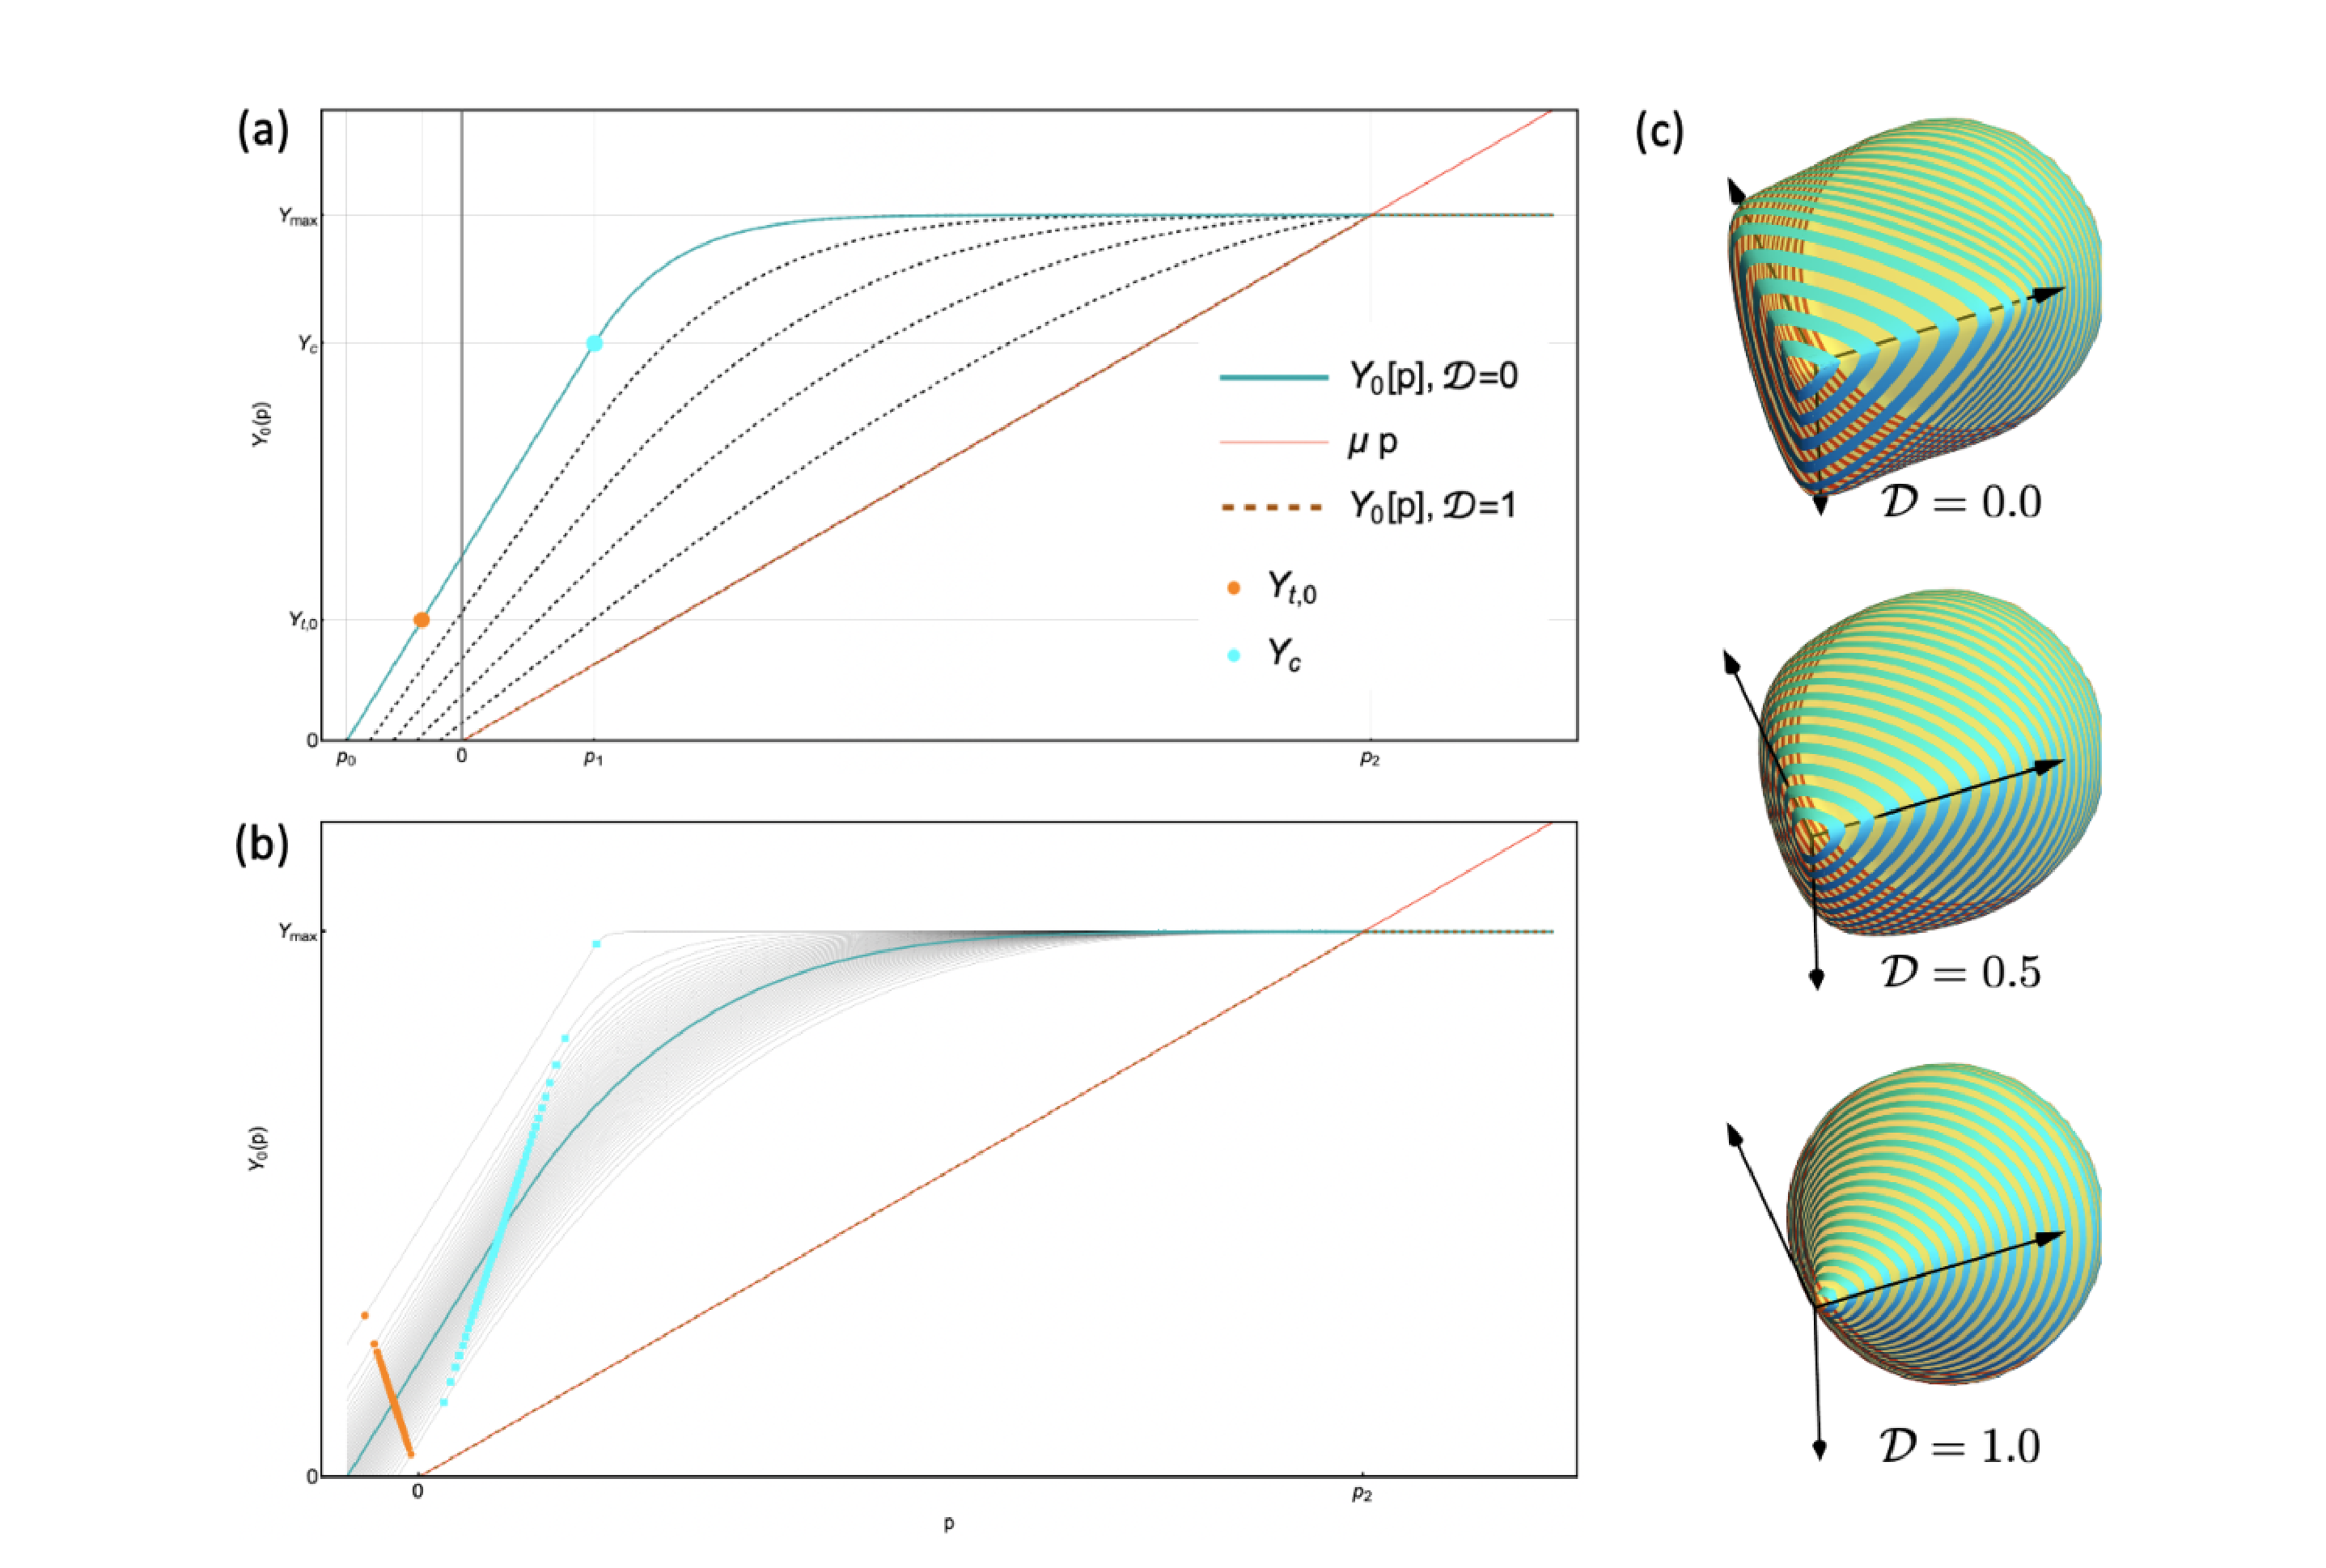
\includegraphics[width=0.92\linewidth]{figures/ceramic_damage_yield_surface_fig8_hi.pdf}
  \caption{Yield surface used by the isotropic ceramic damage model.  Panel (a) shows the pressure-dependent meridional strength without third-invariant dependence, evolving from intact to damaged states.  Panel (b) shows Weibull/strength-scale perturbations of the tensile and compressive strengths subject to the high-pressure cap.  Panel (c) shows the initial principal-stress-space surface for several damage values, illustrating the transition from low-pressure tensile failure toward high-pressure shear strength.  Adapted from Fig.~8 of Homel, Crook, and Appleton~\cite{homelCrookAppleton2026sizeeffects}.}
  \label{fig:ceramic-damage-yield-surface}
\end{figure}

\paragraph{Return mapping.}
The implementation uses a simple radial return in deviatoric stress.  After the pressure branch is selected, the trial deviatoric direction is retained and the returned shear magnitude is limited by the damaged strength,
\begin{equation}
  q^{n+1}=\min\left(q^{\mathrm{tr}},Y(p^{\mathrm{tr}},D,J_2,J_3)/\xi_{\mathrm{tip}}\right),
  \qquad
  \boldsymbol{\sigma}^{n+1}=-p^{n+1}\mathbf{I}+\frac{q^{n+1}}{q^{\mathrm{tr}}}\mathbf{s}^{\mathrm{tr}}.
  \label{eq:ceramic-radial-return}
\end{equation}
The elastic strain energy stored at the returned state is evaluated as
\begin{equation}
  W_e = \frac{(p^{n+1})^2}{2K_{\mathrm{eff}}}+\frac{(q^{n+1})^2}{6G},
  \label{eq:ceramic-elastic-energy}
\end{equation}
which is used by the energy-regularized damage path.  The stored \texttt{plasticStrain} is a diagnostic/history measure computed from the difference between the elastic strain increment implied by the stress change and the total strain increment; it should not be interpreted as a fully associative plastic-flow solution.

\paragraph{Damage regularization options.}
Two damage-progression paths are implemented.  The older time-to-failure path is selected when \texttt{enableEnergyFailureCriterion=0}.  If the trial state yields below the brittle-ductile transition pressure \(p_2\), damage increases according to
\begin{equation}
  D^{n+1}=\min\left(1,D^n+\frac{\Delta t}{t_f}\right),
  \qquad
  t_f=\frac{\ell_{\mathrm{ch}}}{c_f},
  \label{eq:ceramic-time-to-failure}
\end{equation}
where \(\ell_{\mathrm{ch}}=\texttt{lengthScale}\) and \(c_f=\texttt{crackSpeed}\).  This is computationally inexpensive and useful for simple damage growth studies, but the fracture energy is controlled only indirectly by \(c_f\), \(\ell_{\mathrm{ch}}\), and the stress history.

The energy-regularized path is selected when \texttt{enableEnergyFailureCriterion=1}.  In that branch the model tracks accumulated stress work \(W\) and compares the dissipated work \(W-W_e\) to the regularized fracture-energy density \(G_f/\ell_{\mathrm{ch}}\):
\begin{equation}
  D^{n+1}\approx
  \operatorname{clip}\left(\frac{W^{n+1}-W_e^{n+1}}{G_f/\ell_{\mathrm{ch}}},D^n,1\right).
  \label{eq:ceramic-energy-damage}
\end{equation}
If the strain energy at failure is small enough for a gradual softening process, the update performs a fixed-point iteration on \(D\).  If the strain energy at the failure stress already exceeds the target fracture dissipation for the current \(\ell_{\mathrm{ch}}\), the update instead uses a bisection solve for a partially relaxed damage state and sets \texttt{surfaceFlag=1} once the dissipated work reaches approximately \(G_f/\ell_{\mathrm{ch}}\).  That flag is what makes the option useful with DFG: the continuum law can release only the required amount of energy, while the kinematic enrichment creates a contact-capable fracture surface so the residual elastic energy drives opening or slip rather than being smeared into a continuum porosity field.  The regularization concept follows the Homel-Crook-Appleton kinematic-regularization discussion, in which damage, surface insertion, and the energy budget are decoupled when a cell is too large to resolve the fracture process zone~\cite{homelCrookAppleton2026sizeeffects}.

\paragraph{Strength scale and crack-tip scaling.}
The \texttt{strengthScale} field is applied directly to \(Y_t\) and \(Y_c\), so Weibull or spatial heterogeneity assigned by PFW affects both tensile and compressive branches while leaving \(Y_{\max}\) as the limiting ductile strength.  This is the model-specific interpretation of the shared strength-scale field described in Section~\ref{subsubsec:strength-scale-weibull}.  In DFG fracture calculations, \texttt{strengthScale} is commonly assigned by Voronoi/Weibull wrappers so that the initial critical flaws occupy clusters of particles rather than isolated particles.

When crack-tip scaling is enabled, the solver supplies \texttt{distanceToCrackTip} from the neighbor-list DFG crack-tip diagnostic.  The model computes a fracture-process-zone radius from the nominal intact strength,
\begin{equation}
  r_p = \frac{K_{Ic}^{2}}{2\pi Y_{\text{intact}}^{2}},
  \qquad
  \xi_{\mathrm{tip}} = \max\left(1,\sqrt{\frac{r}{r_p}}\right),
  \label{eq:ceramic-crack-tip-factor}
\end{equation}
and divides the effective strength by \(\xi_{\mathrm{tip}}\) when evaluating the yield condition and the return surface.  The stress that is stored and used in momentum balance is not multiplied by this factor; the factor modifies the damage/fracture criterion to represent under-resolved near-tip stresses.  This links the ceramic model to the shared crack-tip modifier in Section~\ref{subsubsec:crack-tip-stress-concentration}.  The uploaded Homel-Crook-Appleton manuscript describes the same idea: the crack-tip factor affects the propagation criterion, while the final output stress and stress work are computed with the unscaled stress~\cite{homelCrookAppleton2026sizeeffects}.

\paragraph{DFG use and porosity interpretation.}
The model can run without DFG, but its intended brittle-fracture workflow is \texttt{CeramicDamage}+DFG.  Without DFG, a fully damaged region remains a continuum carried by the single MPM velocity field and can smear damaged/intact kinematics.  With DFG, particles near a sufficiently sharp damage gradient can be split into two velocity fields, and the contact algorithm then supplies frictional slip and separation on the inserted fracture.  This is important for ceramics, concrete mesostructures, and brittle granular aggregates, where post-failure deformation is often controlled by relative motion of rough fracture faces or fragments.  The \texttt{porosity} field in \texttt{CeramicDamage} currently scales strength through Eq.~\eqref{eq:ceramic-strength-porosity-scale}; it should not be used as the primary representation of dilation caused by fracture slip.  If the problem requires an evolving continuum porosity, pore-pressure coupling, pore collapse, or compaction-induced void-ratio evolution, use or extend \texttt{Geomechanics} (Section~\ref{subsubsec:geomechanics-model}) rather than interpreting DFG fracture dilation as a scalar porosity increment.

\clearpage
\paragraph{Implementation pseudocode.}\mbox{}\par\smallskip
\begin{lstlisting}[caption={CeramicDamage update structure.},label={alg:ceramic-damage-update},basicstyle=\ttfamily\small]
read D, J, lengthScale, strengthScale, porosity, distanceToCrackTip
Yt = strengthScale * (1 - porosity) * tensileStrength
Yc = strengthScale * (1 - porosity) * compressiveStrength
cap Yc by maximumStrength and form Yt0 for optional third-invariant scaling
p_trial = -K_eff(D,J) * log(J)
q_trial, J2, J3, s_hat = deviatoric_invariants(trialStress)
Y_intact = strength(p_trial, D=0, xi=1, J2, J3)
if crack_tip_option and distanceToCrackTip > 0:
  rp = fractureToughness^2 / (2*pi*Y_intact^2)
  xi = max(1, sqrt(distanceToCrackTip / rp))
else:
  xi = 1
Y = strength(p_trial, D, xi, J2, J3)
if p_trial >= (1-D)*p0 and q_trial <= Y:
  accept trial stress
  if energy criterion: accumulatedWork += stress : strainIncrement
else:
  if energy criterion:
    iterate D so (accumulatedWork - elasticEnergy) ~= Gf/lengthScale
    if target dissipation reached: surfaceFlag = 1
  else:
    if p_trial < maximumStrength/frictionSlope:
      D = min(1, D + dt / (lengthScale/crackSpeed))
  radial_return_to_strength_surface(D, xi)
update plasticStrain diagnostic and store stress, D, work, surfaceFlag
\end{lstlisting}

\subsubsection{\texttt{Chiumenti}}
\label{subsubsec:chiumenti-model}
\index{constitutiveModels!Chiumenti}
\index{Rankine damage}

\texttt{Chiumenti} is a scalar tensile-damage model built on the \texttt{HyperelasticMMS} trial stress.  It follows the local continuum damage / crack-band style of Rankine tensile softening used in the work of Cervera and Chiumenti~\cite{cervera2006chiumenti}.  In GEOS-MPM, it provides a compact hyperelastic-damage option for cases that require tensile degradation with a characteristic length and fracture-energy parameter, but not the full ceramic or geomechanics response.

The model computes a hyperelastic trial stress, obtains principal stresses \(\sigma_i\), and defines a strength
\begin{equation}
  Y_f = s_p Y_{f0},
\end{equation}
where \(s_p\) is the particle \texttt{strengthScale}.  With Young's modulus \(E\), critical length \(\ell_c\), and energy-release parameter \(G_f\), the implementation uses a brittleness factor
\begin{equation}
  b = \frac{Y_f^2}{2 E G_f},
  \qquad
  b_c = \frac{b\ell_c}{1-b\ell_c}.
  \label{eq:chiumenti-brittleness}
\end{equation}
When the maximum tensile principal stress \(\sigma_{\max}\) exceeds \(Y_f\), the damage candidate is
\begin{equation}
  D_{\mathrm{new}}
  = (1+b_c)\left(1-\frac{Y_f}{\sigma_{\max}}\right),
  \qquad
  D^{n+1}=\max\left(D^n,\min(1,\max(0,D_{\mathrm{new}}))\right).
  \label{eq:chiumenti-damage}
\end{equation}
Positive principal stresses are then degraded by \(1-D\), while compressive principal stresses are left unchanged.

\begin{lstlisting}[caption={Chiumenti tensile-damage update.},label={alg:chiumenti-update},basicstyle=\ttfamily\small]
stress_trial = HyperelasticMMS(F)
if inelasticity disabled: return stress_trial
Yf = failureStrength * strengthScale
principalStress, eigenvectors = eig(stress_trial)
sigmaMax = max(max(principalStress), 0)
if sigmaMax > Yf:
  b = Yf^2 / (2 * E * energyReleaseRate)
  bc = b * criticalLength / (1 - b * criticalLength)
  damage = max(oldDamage, clamp((1 + bc) * (1 - Yf/sigmaMax), 0, 1))
for each principal stress i:
  if principalStress[i] > 0: principalStress[i] *= (1 - damage)
stress = recompose(principalStress, eigenvectors)
\end{lstlisting}
\subsubsection{\texttt{Graphite}}
\label{subsubsec:graphite-model}
\index{constitutiveModels!Graphite}
\index{Graphite model}
\index{MaterialDirection!Graphite}
\index{transverse isotropy!Graphite}
\index{graphite!weak planes}
\index{graphite!basal planes}
\index{graphite!point-slope strength}

\texttt{Graphite} is an anisotropic damage/plasticity model for graphite-like layered solids.  The model assumes that the material has a preferred graphitic or basal-plane normal, stored as the first row of the particle \texttt{MaterialDirection} tensor.  The weak planes themselves are normal to this vector.  The constitutive update therefore treats the particle material direction as a plane normal, not as an ordinary fiber tangent.  This distinction matters in large deformation: ordinary line directions are pushed forward with \(\mathbf F\), while plane normals are pushed forward with the deformation-gradient cofactor \(\mathbf F^{c}=J\mathbf F^{-T}\).  The MPM kinematic update uses this cofactor path for non-fiber material directions, normalizes the transported rows, and then passes the updated material basis to the constitutive model.  This is the appropriate graphitic update because the orientation of a basal plane is controlled by the transformed plane normal rather than by the stretch of an in-plane material line; see also the material-direction assignment discussion in Section~\ref{subsec:pfw-material-directions}.  The need to distinguish material rotations, basis transformations, and evolving anisotropy is the same tensor-transformation issue emphasized by Brannon's rotation and frame-change treatment~\cite{brannon2017rotation}.

\begin{figure}[htbp]
  \centering
  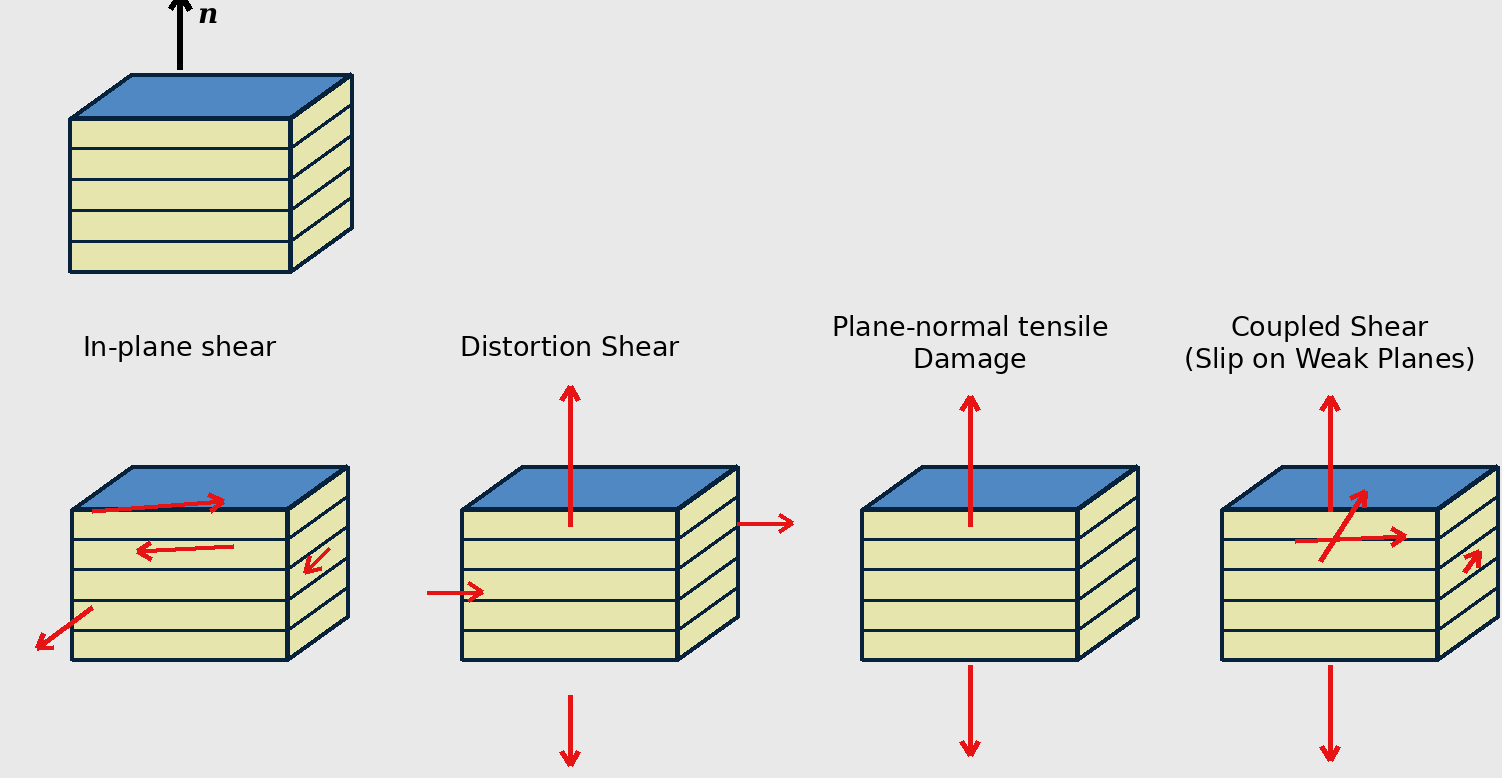
\includegraphics[width=0.96\linewidth]{figures/graphite_deformation_modes.png}
  \caption{Graphite weak-plane deformation modes.  The supplied diagram illustrates the basal-plane normal, in-plane shear, distortion shear, plane-normal tensile damage, and coupled shear/slip on weak planes.  The assigned material direction \(\mathbf a\) is the normal to the weak graphitic planes; in-plane, distortion, plane-normal, and coupled weak-plane stress modes are limited by separate pressure-dependent strength functions.}
  \label{fig:graphite-deformation-modes}
\end{figure}

\paragraph{Kinematics and material basis.}
Let \(\mathbf a\) be the current unit normal to the graphitic planes and let
\begin{equation}
  \mathbf M = \mathbf a\otimes\mathbf a,
  \qquad
  \mathbf P = \mathbf I - \mathbf M,
  \label{eq:graphite-projectors}
\end{equation}
where \(\mathbf P\) projects onto the basal plane.  In the current implementation the full particle material basis is stored row-wise, but the constitutive update uses only the first row as \(\mathbf a\).  The solver first transports the reference basis by
\begin{equation}
  \mathbf A^{\mathrm{trial}} =
  \begin{cases}
    \mathbf F\mathbf A_0^T, & \hbox{fiber-like material directions},\\
    \mathbf F^{c}\mathbf A_0^T, & \hbox{graphitic plane normals and other non-fiber directions},
  \end{cases}
  \qquad
  \mathbf F^{c}=J\mathbf F^{-T},
  \label{eq:graphite-material-direction-update}
\end{equation}
then transposes and normalizes the rows to recover the particle \texttt{MaterialDirection}.  Inside the constitutive update, the beginning-of-step rotation is removed before evaluating the transversely isotropic elastic and inelastic laws, so the mode decomposition is performed in a corotational material frame.  This path is consistent with the general rule that anisotropic constitutive models must evolve their material directions under superposed rigid motion and finite distortion, rather than treating a fixed laboratory axis as a material property~\cite{brannon2017rotation}.

\paragraph{Elastic trial stress.}
The reviewed code path is a finite-deformation MPM update followed by a corotational transversely isotropic elastic predictor.  The implementation is compatible with the hyperelastic transversely isotropic interpretation of the model, but the update evaluated here is algorithmically a pressure-dependent rate-form trial stress expressed in the evolving material frame.  The pressure-dependent moduli are computed from the beginning-of-step pressure \(p^n=-\operatorname{tr}\boldsymbol{\sigma}^n/3\) and the beginning-of-step plane-normal stress \(\sigma_n^n=\mathbf a\cdot\boldsymbol{\sigma}^n\mathbf a\).  Define the non-negative arguments
\begin{equation}
  \xi_z = \max\left(0,\frac{p^n-\sigma_n^n}{2}\right),
  \qquad
  \xi_p = \max(0,p^n),
  \label{eq:graphite-elastic-pressure-arguments}
\end{equation}
and the saturating pressure function
\begin{equation}
  f(\xi;P)=\frac{\xi}{1+\xi/P}.
  \label{eq:graphite-saturating-pressure-function}
\end{equation}
Then
\begin{align}
  E_z &= \max\left(10^{-3}E_z^0,
       E_z^0 + E_z' f(\xi_z;P_z)\right),\\
  E_p &= \max\left(10^{-3}E_p^0,
       E_p^0 + E_p' f(\xi_p;P_p)\right),\\
  G_{zp} &= \max\left(10^{-3}G_{zp}^0,
       G_{zp}^0 + G_{zp}' f(\xi_p;P_g)\right),\\
  \nu_{zp} &= \min(0.4999,\nu_{zp}^0),
  \qquad
  \nu_p = \min(0.4999,\nu_p^0).
  \label{eq:graphite-pressure-dependent-moduli}
\end{align}
Here \(z\) denotes the preferred-axis direction and \(p\) denotes the transverse plane.  The optional pressure scales \(P_z\), \(P_p\), and \(P_g\) are supplied by \texttt{defaultYoungModulusAxialPressureScale}, \texttt{defaultYoungModulusTransversePressureScale}, and \texttt{defaultShearModulusAxialTransversePressureScale}.  When a pressure scale is omitted, its default is effectively infinite and \(f(\xi;P)\to\xi\), recovering the linear pressure dependence.  Finite positive scales give monotone pressure stiffening with decreasing tangent modulus increment at high pressure.  The implementation also locally limits the pressure-dependent TI moduli if needed so the stiffness remains positive definite at the current pressure state.  The implementation also forms effective isotropic moduli for wave-speed and stress-control purposes,
\begin{equation}
  K_{\mathrm{eff}} =
  -\frac{E_pE_z}{2E_z(\nu_p+\nu_{zp}-1)+E_p(2\nu_{zp}-1)},
  \qquad
  G_{\mathrm{eff}} = 0.6K_{\mathrm{eff}}.
  \label{eq:graphite-effective-moduli}
\end{equation}

The elastic stiffness is written using the five transversely isotropic fourth-order basis tensors associated with the symmetry axis \(\mathbf a\).  Brannon gives the corresponding TI basis and discusses the physical meaning of these components as axial response, in-plane isotropic response, Poisson coupling, in-plane shear, and shear involving the symmetry axis~\cite{brannon2017rotation}.  In component form, with \(a_i\) denoting the components of \(\mathbf a\),
\begin{align}
  B^{(1)}_{ijpw} &= a_i a_j a_p a_w,\\
  B^{(2)}_{ijpw} &= \delta_{ij}\delta_{pw}
      -a_i a_j\delta_{pw}-\delta_{ij}a_p a_w+a_i a_j a_p a_w,\\
  B^{(3)}_{ijpw} &= a_i a_j\delta_{pw}+\delta_{ij}a_p a_w
      -2a_i a_j a_p a_w,\\
  B^{(4)}_{ijpw} &= \frac{1}{2}\left(\delta_{ip}\delta_{jw}+\delta_{iw}\delta_{jp}\right)
      -\frac{1}{2}\left(\delta_{iw}a_j a_p+a_i\delta_{jp}a_w+a_i\delta_{jw}a_p+\delta_{ip}a_j a_w\right)
      +a_i a_j a_p a_w,\\
  B^{(5)}_{ijpw} &= \frac{1}{2}\left(\delta_{ip}a_j a_w+\delta_{iw}a_j a_p+a_i\delta_{jw}a_p+a_i\delta_{jp}a_w\right)
      -2a_i a_j a_p a_w.
  \label{eq:graphite-ti-basis}
\end{align}
The stiffness used by the trial update is
\begin{equation}
  \mathbb C_{\mathrm{TI}} = h_1\mathbb B^{(1)}+h_2\mathbb B^{(2)}+h_3\mathbb B^{(3)}+h_4\mathbb B^{(4)}+h_5\mathbb B^{(5)},
  \label{eq:graphite-ti-stiffness}
\end{equation}
with
\begin{align}
  h_1 &= \frac{E_z^2(\nu_p-1)}{E_z(\nu_p-1)+2E_p\nu_{zp}^2},
  &
  h_2 &= -\frac{E_p(E_z\nu_p+E_p\nu_{zp}^2)}{(1+\nu_p)\left[E_z(\nu_p-1)+2E_p\nu_{zp}^2\right]},\\
  h_3 &= \frac{E_pE_z\nu_{zp}}{E_z-E_z\nu_p-2E_p\nu_{zp}^2},
  &
  h_4 &= \frac{E_p}{1+\nu_p},
  &
  h_5 &= 2G_{zp}.
  \label{eq:graphite-h-coefficients}
\end{align}
The trial stress increment is
\begin{equation}
  \Delta\boldsymbol{\sigma}^{\mathrm{tr}}
  = \mathbb C_{\mathrm{TI}}:
  \left(\mathbf D - \boldsymbol{\alpha}\dot T\right)\Delta t,
  \qquad
  \boldsymbol{\alpha} = (\alpha_L-\alpha_T)\mathbf a\otimes\mathbf a+\alpha_T\mathbf I,
  \label{eq:graphite-trial-stress}
\end{equation}
where \(\dot T=\texttt{temperatureRate}\).  Thus thermal expansion is anisotropic: \(\alpha_L\) is applied along the symmetry-axis normal and \(\alpha_T\) in the basal plane.  In current GEOS-MPM workflows, \texttt{temperature} and \texttt{temperatureRate} are generally prescribed by global solver events that define a transient thermal response; the graphite update consumes these fields to represent thermal expansion and temperature-dependent properties.  A future coupled heat-transfer solver could instead define local particle temperature and temperature-rate fields.

\paragraph{Mode decomposition of stress.}
After the trial stress is computed, the model decomposes it into four symmetric tensor parts.  In the notation of Eq.~\eqref{eq:graphite-ti-basis},
\begin{align}
  \boldsymbol{\sigma}_1 &= \mathbb B^{(1)}:\boldsymbol{\sigma},
  &\hbox{plane-normal/axial part},\\
  \boldsymbol{\sigma}_2 &= \mathbb B^{(2)}:\boldsymbol{\sigma},
  &\hbox{in-plane isotropic part before the factor }1/2,\\
  \boldsymbol{\sigma}_4 &= \mathbb B^{(4)}:\boldsymbol{\sigma},
  &\hbox{in-plane total part},\\
  \boldsymbol{\sigma}_5 &= \mathbb B^{(5)}:\boldsymbol{\sigma},
  &\hbox{coupled weak-plane shear part}.
  \label{eq:graphite-stress-parts}
\end{align}
The in-plane isotropic contribution used for reconstruction is \(\boldsymbol{\sigma}_{\mathrm{ip}}^{\mathrm{iso}}=\boldsymbol{\sigma}_2/2\), while the in-plane deviator is
\begin{equation}
  \boldsymbol{\sigma}_{\mathrm{ip}}^{\mathrm{dev}} = \boldsymbol{\sigma}_4 - \frac{1}{2}\boldsymbol{\sigma}_2 .
  \label{eq:graphite-inplane-dev}
\end{equation}
The distortion stress is the combination of the plane-normal and in-plane-isotropic parts,
\begin{equation}
  \boldsymbol{\sigma}_{\mathrm{dist}} = \boldsymbol{\sigma}_1 + \frac{1}{2}\boldsymbol{\sigma}_2,
  \qquad
  \boldsymbol{\sigma}_{\mathrm{dist}}^{\mathrm{dev}} =
  \operatorname{dev}\boldsymbol{\sigma}_{\mathrm{dist}}.
  \label{eq:graphite-distortion-stress}
\end{equation}
The signed distortion invariant is
\begin{equation}
  I_d = \sigma_{aa} - \frac{\sigma_{bb}+\sigma_{cc}}{2},
  \qquad
  I_d^+ = \langle I_d\rangle_+,
  \qquad
  I_d^- = \langle -I_d\rangle_+,
  \label{eq:graphite-signed-distortion}
\end{equation}
where \(\mathbf a\) is the basal-plane normal and \(\mathbf b,\mathbf c\) span the basal plane.  The scalar \(|I_d|\) is equal to \(\sqrt{3/2}\|\boldsymbol{\sigma}_{\mathrm{dist}}^{\mathrm{dev}}\|\), but the split form allows the model to assign different strengths to basal-normal relative compression and basal-normal relative extension/opening-like distortion.  The remaining mode invariants use Mandel-consistent norms,
\begin{equation}
  q_{\mathrm{ip}} = \sqrt{\frac{3}{2}}\,\|\boldsymbol{\sigma}_{\mathrm{ip}}^{\mathrm{dev}}\|,
  \qquad
  q_{\mathrm{c}} = \sqrt{\frac{3}{2}}\,\|\boldsymbol{\sigma}_5\|.
  \label{eq:graphite-mode-invariants}
\end{equation}
These are the internal stress measures corresponding to signed normal distortion, in-plane shear, and coupled shear on the graphitic weak planes in Fig.~\ref{fig:graphite-deformation-modes}.  Plane-normal tensile opening is handled separately by comparing \(\sigma_n=\mathbf a\cdot\boldsymbol{\sigma}\mathbf a\) with \texttt{failureStrength}.

\paragraph{Pressure-dependent point-slope strengths.}
Each active strength branch \(m\in\{d-,d+,\mathrm{ip},\mathrm{c}\}\) has a pressure-dependent strength curve controlled by \texttt{*ResponseX2}, \texttt{*ResponseY1}, \texttt{*ResponseY2}, and \texttt{*ResponseM1}.  The existing \texttt{distortionShearResponse*} inputs define the \(I_d^-\) branch.  The optional \texttt{positiveDistortionShearResponse*} inputs define the \(I_d^+\) branch and default to the corresponding \texttt{distortionShearResponse*} values when omitted, so old input files recover the previous unsigned distortion response.  With \(x_1=0\), \(x_2>0\), \(Y_1\ge 0\), \(Y_2>Y_1\), and low-pressure tangent slope \(M_1\), the code uses a point-slope form
\begin{equation}
Y_m(p)=
\begin{cases}
  \max\left(0, Y_1-(x_1-p)M_1\right), & p<x_1,\\[0.4em]
  Y_2+(Y_1-Y_2)\left(\dfrac{p-x_2}{x_1-x_2}\right)^{M_1(x_1-x_2)/(Y_1-Y_2)}, & x_1\le p < x_2,\\[0.8em]
  Y_2, & p\ge x_2.
\end{cases}
\label{eq:graphite-point-slope-strength}
\end{equation}
This curve passes through \((x_1,Y_1)\) with derivative \(M_1\), passes through \((x_2,Y_2)\), and is tangent to the high-pressure branch, which is a zero-slope plateau in the present form.  The elastic domain is convex only if the low-pressure slope is steeper than the secant slope, so the intended parameter regime is
\begin{equation}
  M_1 > \frac{Y_2-Y_1}{x_2-x_1}.
  \label{eq:graphite-point-slope-convexity}
\end{equation}
After damage and hardening modifications the implementation enforces this condition by increasing \(M_1\) when needed, with a small numerical margin in production inputs preferred over exact equality.

\begin{figure}[htbp]
  \centering
  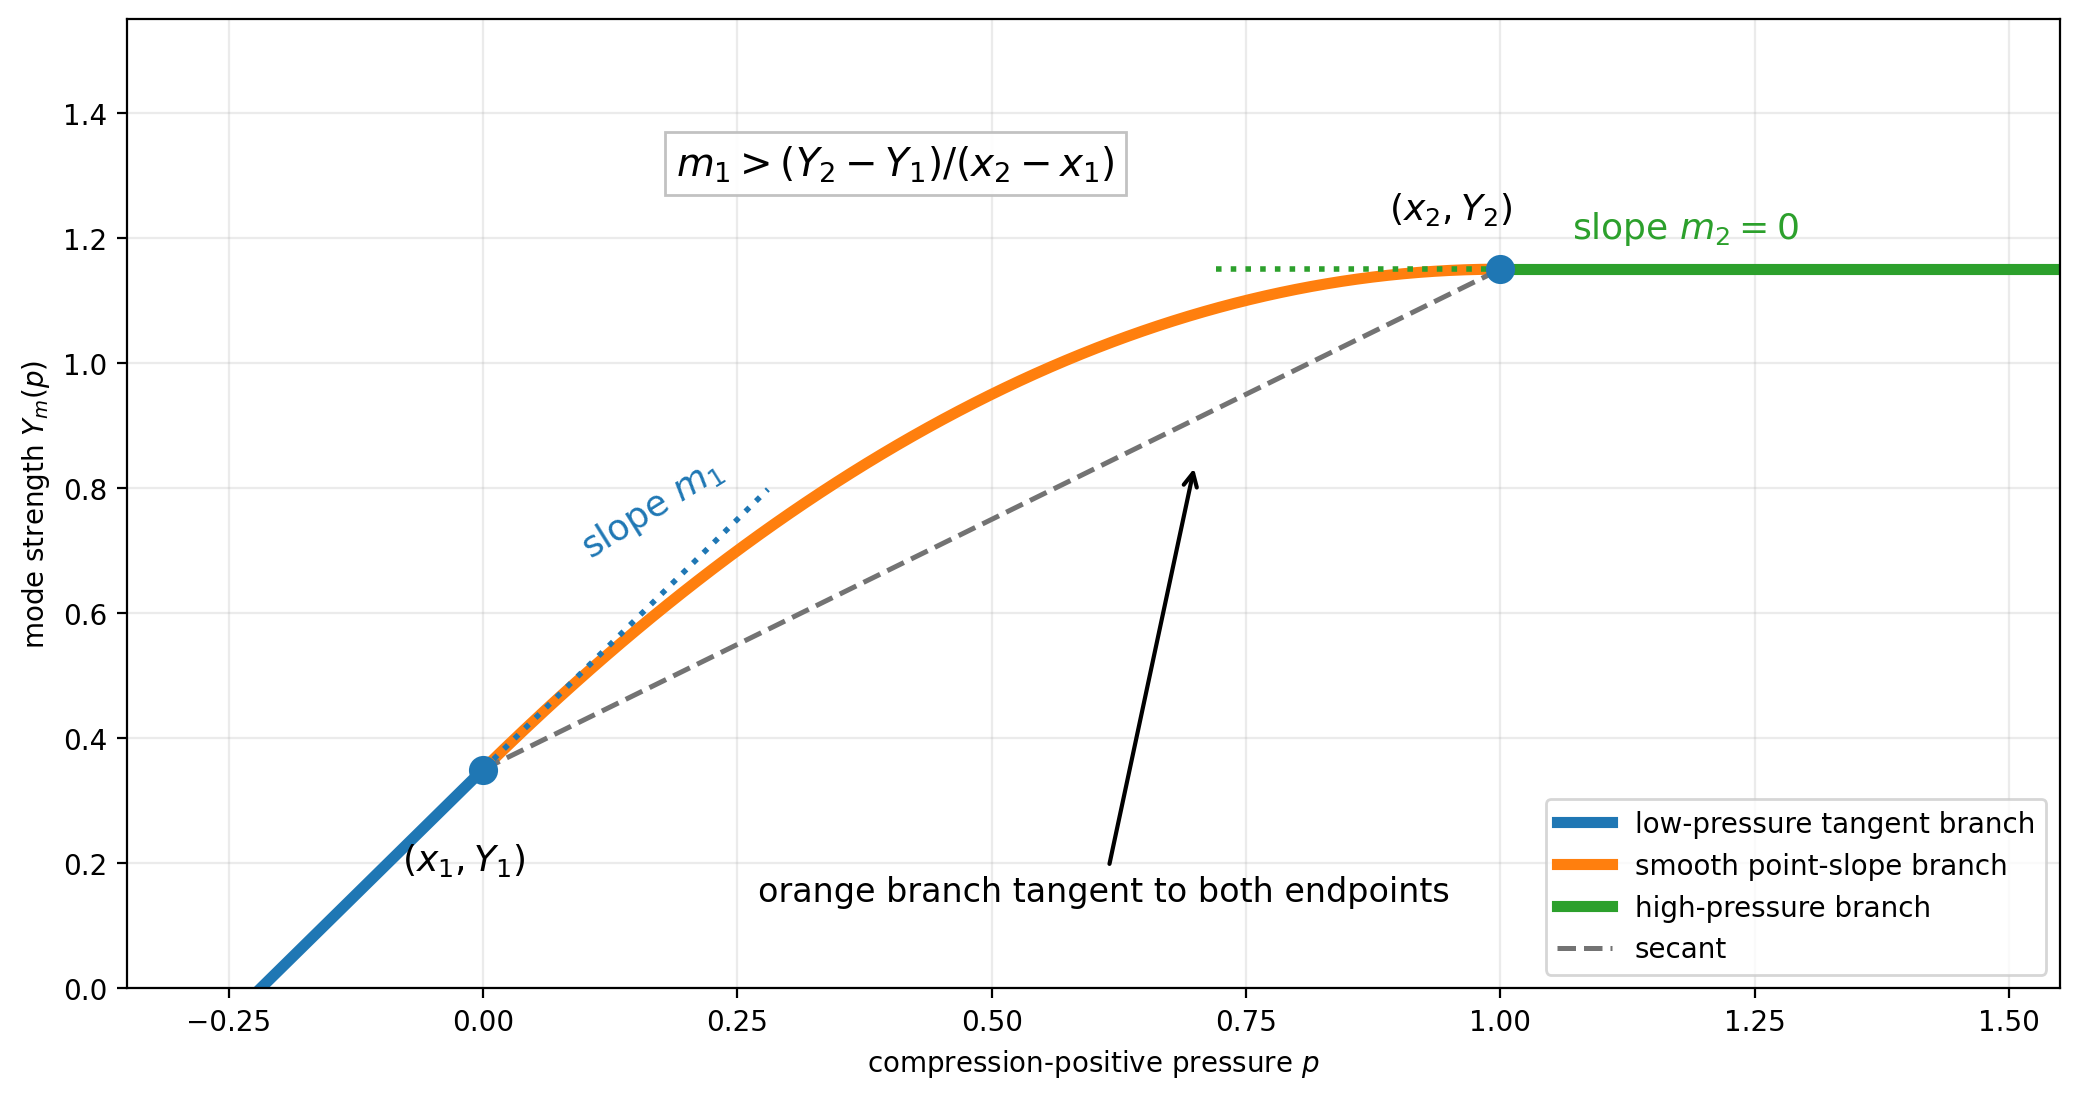
\includegraphics[width=0.78\linewidth]{figures/graphite_point_slope_strength.png}
  \caption{Pressure-dependent point-slope strength form used for each active graphite strength branch, including the signed distortion branches, in-plane shear, and coupled weak-plane shear.  The orange transition is constructed to be tangent to the low-pressure branch at \((x_1,Y_1)\) and tangent to the high-pressure plateau at \((x_2,Y_2)\); convexity requires \(M_1>(Y_2-Y_1)/(x_2-x_1)\).}
  \label{fig:graphite-point-slope-strength}
\end{figure}

Damage, strength scaling, and hardening modify the raw input strengths before Eq.~\eqref{eq:graphite-point-slope-strength} is evaluated.  Let \(s_p=\texttt{strengthScale}\), \(D_m\in[0,1]\) be the internal mode damage used for a branch, \(\chi=\texttt{relaxation}\in[0,1]\) be the accumulated plastic-strain hardening coordinate, and
\begin{equation}
  S(\chi)=3\chi^2-2\chi^3,
  \qquad
  H_m(\chi)=1+(C_m-1)S(\chi).
  \label{eq:graphite-hardening-multiplier}
\end{equation}
Here \(C_m\) is one of \texttt{distortionStrainHardeningC0}, \texttt{inPlaneStrainHardeningC0}, or \texttt{coupledStrainHardeningC0}; both signed distortion branches use the distortion hardening multiplier.  The intact low-pressure ordinate and tangent slope are scaled by \(s_pH_m\), but the high-pressure plateau is not strength-scale multiplied:
\begin{equation}
  Y_{1,\mathrm{intact}} = \min\left(s_pH_mY_1^0,(1-\epsilon)Y_2^0\right),
  \qquad
  Y_{2,\mathrm{intact}} = Y_2^0.
  \label{eq:graphite-strengthscale-damage}
\end{equation}
The intact slope is raised as needed to satisfy the convexity condition in Eq.~\eqref{eq:graphite-point-slope-convexity}.  The fully comminuted powder branch has zero cohesion, uses \texttt{damagedMaterialFrictionalSlope} subject to the same slope limits, and retains the same unscaled branch-specific \(Y_2^0\) plateau.  The active strength is a smooth blend of the intact and powder branches using the internal damage variable for that mode.  This makes \texttt{strengthScale} a flaw-controlled low-pressure multiplier while preserving a common pressure-dominated high-confinement strength for intact and comminuted material.  Fracture energies may be scaled separately through \(G_f^{\mathrm{eff}}=G_f\,s_p^{\eta_G}\), where \(\eta_G=\texttt{fractureEnergyStrengthScaleExponent}\).

\paragraph{Mode return and reconstruction.}
The inelastic correction uses a single quadratic TI strength index,
\begin{equation}
  R^2 =
  \left(\frac{I_d^+}{Y_{d+}(p)}\right)^2+
  \left(\frac{I_d^-}{Y_{d-}(p)}\right)^2+
  \left(\frac{q_{\mathrm{ip}}}{Y_{\mathrm{ip}}(p)}\right)^2+
  \left(\frac{q_{\mathrm{c}}}{Y_{\mathrm{c}}(p)}\right)^2 .
  \label{eq:graphite-quadratic-ti-yield}
\end{equation}
When \(R>1\), the deviatoric distortion, in-plane, and coupled weak-plane stress parts are scaled by \(1/R\).  This is a radial projection onto a coupled anisotropic strength index rather than a full closest-point plasticity return.  After the correction, the stress is reconstructed as
\begin{equation}
  \boldsymbol{\sigma}^{n+1} =
  \boldsymbol{\sigma}_{\mathrm{dist}}^{\mathrm{iso}}
  + \boldsymbol{\sigma}_{\mathrm{dist}}^{\mathrm{dev,capped}}
  + \boldsymbol{\sigma}_{\mathrm{ip}}^{\mathrm{dev,capped}}
  + \boldsymbol{\sigma}_{5}^{\mathrm{capped}}.
  \label{eq:graphite-stress-reconstruction}
\end{equation}
For fully damaged particles, the implementation also removes tensile plane-normal stress and spherical tensile distortion stress, so the damaged material can continue to carry compressive/frictional response but cannot support cohesive opening strength.

\paragraph{Plastic strain, hardening, and damage evolution.}
When at least one mode cap is active, the model computes a plastic strain increment by subtracting the elastic strain increment implied by the TI compliance from the total symmetric velocity-gradient increment.  The TI compliance uses coefficients
\begin{equation}
  s_1=\frac{1}{E_z},\qquad
  s_2=-\frac{\nu_p}{E_p},
  \qquad
  s_3=-\frac{\nu_{zp}}{E_z},
  \qquad
  s_4=\frac{1+\nu_p}{E_p},
  \qquad
  s_5=\frac{1}{2G_{zp}}.
  \label{eq:graphite-compliance-coefficients}
\end{equation}
The relaxation/hardening coordinate is then advanced approximately as
\begin{equation}
  \chi^{n+1}=\min\left(1,\chi^n+\frac{\|\Delta\boldsymbol{\epsilon}^p\|}{\epsilon^p_{\max}}\right),
  \label{eq:graphite-relaxation-update}
\end{equation}
where \(\epsilon^p_{\max}=\texttt{maximumPlasticStrain}\).  This history variable is the argument in Eq.~\eqref{eq:graphite-hardening-multiplier}.

Damage can evolve through several mechanisms.  First, when \texttt{maximumPrincipalStressDamage=1}, the model evaluates the largest principal stress and advances damage if
\begin{equation}
  C_{\mathrm{tip}}\,\sigma_{\max} > s_p\,\sigma_f,
  \label{eq:graphite-maxprincipal-damage}
\end{equation}
where \(\sigma_f=\texttt{failureStrength}\) and \(C_{\mathrm{tip}}=\texttt{crackTipStressConcentration}\).  The crack-tip multiplier is produced by the shared crack-tip modifier described in Section~\ref{subsubsec:crack-tip-stress-concentration}.  Second, if \texttt{crackSpeed} is finite and an inelastic correction has occurred, damage advances over the time-to-failure scale
\begin{equation}
  \Delta D = \frac{\Delta t}{\ell/c_f},
  \qquad
  \ell=\texttt{lengthScale},
  \quad c_f=\texttt{crackSpeed}.
  \label{eq:graphite-crackspeed-damage}
\end{equation}
Third, the model accumulates basal-plane plastic work and non-basal plastic work.  The basal work combines Mode-I basal-plane plastic opening work and basal-plane shear work; the total work path excludes the basal plane-normal and basal shear parts.  These work measures are regularized by fracture energy per unit characteristic length,
\begin{equation}
  D \leftarrow \max\left(D,
     \left[\min\left(1,\frac{W_b}{G_b/\ell}\right)\right]^{n_D},
     \left[\min\left(1,\frac{W_t}{G_t/\ell}\right)\right]^{n_D}
  \right),
  \label{eq:graphite-work-damage}
\end{equation}
where \(G_b=\texttt{basalPlaneFractureEnergyReleaseRate}\), \(G_t=\texttt{totalFractureEnergyReleaseRate}\), and \(n_D=\texttt{damageEvolutionExponent}\).  The effective fracture energy uses \(G_f^{\mathrm{eff}}=G_f s_p^{\eta_G}\), where \(\eta_G=\texttt{fractureEnergyStrengthScaleExponent}\).  If the exponent is omitted, the legacy \texttt{scaleFractureEnergyReleaseRate} flag initializes it to either zero or one.  Equation~\eqref{eq:graphite-work-damage} makes damage remain near zero until the accumulated work approaches the specified regularized fracture-work threshold, then ramps it toward one.

\paragraph{Thermal effects.}
Thermal effects in the current model enter through anisotropic thermal expansion in Eq.~\eqref{eq:graphite-trial-stress} and through any temperature-dependent parameter paths exposed by the material model.  In the current solver workflow, \texttt{temperature} and \texttt{temperatureRate} are normally imposed by global events, such as a \texttt{TemperatureProfile} or \texttt{TemperatureRamp}, to represent a prescribed transient thermal response.  The graphite constitutive update consumes \texttt{temperatureRate} to subtract \(\boldsymbol{\alpha}\dot T\) from the mechanical rate of deformation.  Local temperature fields could instead be supplied in the future by a coupled heat-transfer solver, because temperature is already a particle field shared by PFW initialization, events, output, and constitutive models as described in Section~\ref{subsubsec:constitutive-temperature}.

\paragraph{Update algorithm.}
\begin{lstlisting}[caption={Graphite constitutive update structure.},label={alg:graphite-update},basicstyle=\ttfamily\small]
read old stress, velocity gradient, F, materialDirection, damage, temperatureRate
transport/normalize material direction; use first row as basal-plane normal a
unrotate L and a into the corotational material frame
compute pressure p, plane-normal stress sigma_n, and saturating pressure-dependent TI moduli
construct TI stiffness from Brannon basis tensors B1...B5
stress_trial = oldStress + C_TI : (D - alpha * temperatureRate) * dt
if inelasticity is disabled: accept stress_trial

decompose stress_trial into sigma1, sigma2, sigma4, sigma5
compute signed distortion Id+/Id-, in-plane, and coupled shear invariants
compute branch strengths Y_d-, Y_d+, Y_ip, Y_c from point-slope curves
apply strengthScale to low-pressure intact branch only; keep Y2 unscaled
blend intact strengths toward pressure-dependent powder residual using internal damage
if R^2 = sum((mode stress)/(mode strength))^2 > 1: scale deviatoric TI modes by 1/R
reconstruct stress from corrected distortion, in-plane, and coupled parts
as damage grows: remove tensile plane-normal and spherical tensile strength

if any mode yielded:
  compute plastic strain increment from total strain increment minus TI elastic increment
  update relaxation/hardening coordinate
  update max-principal, crack-speed, basal-work, and total-work damage paths
store stress, damage, relaxation, plastic strain, plastic work, and diagnostics
\end{lstlisting}

\paragraph{Capabilities and limitations.}
The model is useful when the important physics are anisotropic graphitic weak planes, pressure-dependent shear strength, basal-plane slip/opening, thermal expansion anisotropy, and coupling to DFG fracture/contact.  It is not a general porous geomaterial model: continuum porosity, pore collapse, pressure-solution creep, and pore-pressure coupling should be handled by the \texttt{Geomechanics} family or by a future coupled model.  It is also not a fully coupled anisotropic plasticity return algorithm with a documented associated flow rule; the correction is a radial projection to a coupled TI strength index.  The strict stored-energy hyperelastic interpretation is likewise limited, because the reviewed code computes a corotational rate-form trial stress.  Finally, the constitutive update uses only the first material-direction row as the basal-plane normal, so users should initialize unused material-basis rows sensibly for robust kinematic transport and output, even though they do not directly alter the graphite strength calculation.

\begingroup
\footnotesize
\begin{longtable}{>{\raggedright\arraybackslash}p{0.44\linewidth}>{\raggedright\arraybackslash}p{0.49\linewidth}}
\caption{Main \texttt{Graphite} input groups.  See the generated schema appendix for exact defaults and registration status.\label{tab:graphite-parameters}}\\
\toprule
\textbf{Input group} & \textbf{Purpose}\\
\midrule
\endfirsthead
\toprule
\textbf{Input group} & \textbf{Purpose}\\
\midrule
\endhead
\texttt{defaultYoungModulusAxial}\newline \texttt{defaultYoungModulusTransverse}\newline \texttt{defaultShearModulusAxialTransverse} & Baseline transversely isotropic elastic moduli along the basal-plane normal, in the basal plane, and in mixed axial-transverse shear.\\
\texttt{defaultPoissonRatioAxialTransverse}\newline \texttt{defaultPoissonRatioTransverse} & Poisson couplings for the TI elastic law.\\
\texttt{*PressureDerivative}\newline \texttt{*PressureScale} & Optional pressure slopes and saturation scales for \(E_z\), \(E_p\), and \(G_{zp}\).  Omitted pressure scales recover the linear pressure dependence.\\
\texttt{failureStrength}\newline \texttt{maximumPrincipalStressDamage}\newline \texttt{enableCrackTipStressConcentration} & Tensile/principal-stress damage controls and crack-tip modifier coupling.\\
\texttt{distortionShearResponse*} & Point-slope parameters for the negative signed-distortion branch \(I_d^-\).\\
\texttt{positiveDistortionShearResponse*} & Optional point-slope parameters for the positive signed-distortion branch \(I_d^+\); omitted values default to \texttt{distortionShearResponse*}.\\
\texttt{inPlaneShearResponse*} & Point-slope parameters for basal-plane in-plane shear.\\
\texttt{coupledShearResponse*} & Point-slope parameters for coupled shear/slip involving the weak plane normal.\\
\texttt{distortionStrainHardeningC0}\newline \texttt{inPlaneStrainHardeningC0}\newline \texttt{coupledStrainHardeningC0}\newline \texttt{maximumPlasticStrain} & Plastic-strain hardening controls through the relaxation coordinate.\\
\texttt{basalPlaneFractureEnergyReleaseRate}\newline \texttt{totalFractureEnergyReleaseRate}\newline \texttt{scaleFractureEnergyReleaseRate}\newline \texttt{crackSpeed} & Damage regularization and rate controls.\\
\texttt{alphaL}\newline \texttt{alphaT}\newline \texttt{temperature}\newline \texttt{temperatureRate} & Anisotropic thermal expansion path.\\
\texttt{materialDirection} & Particle material basis; the first row is the graphitic plane normal used by the constitutive model.\\
\bottomrule
\end{longtable}
\endgroup

\subsubsection{\texttt{Geomechanics}}
\label{subsubsec:geomechanics-model}
\index{constitutiveModels!Geomechanics}
\index{porosity!geomechanics}
\index{Geomechanics model}
\index{Arenisca}
\index{Kayenta}
\index{CB-TSCPR}

\texttt{Geomechanics} is the MPM-connected porous geomaterial model.  It is intended for rocks, chalks, cemented granular media, and other pressure-sensitive materials for which the important continuum mechanisms include nonlinear elasticity, pressure-dependent shear strength, a compaction cap, evolving porosity, strain hardening, brittle damage, optional creep, and nonassociative plastic flow.  The model lineage follows the Arenisca/Kayenta family of cap-plasticity geomodels and the Homel--Guilkey--Brannon consistency-bisection transformed-space closest-point-return (CB-TSCPR) solution strategy~\cite{brannon2009kayenta,homel2014arenisca,homel2015cbtscpr}.  The Ghareb-chalk formulation adds the creep, hardening, damage, and pressure-dependent shear-modulus features summarized below~\cite{malenda2025ghareb}.

The model is distinct from \texttt{CeramicDamage}.  \texttt{CeramicDamage} is primarily a brittle-fracture model intended to work with DFG surfaces and frictional contact, whereas \texttt{Geomechanics} treats porosity, compaction, and cap hardening as continuum state variables.  Use \texttt{Geomechanics} when continuum pore-volume evolution, pressure-sensitive compaction, and creep are part of the material response.  Use the DFG/contact machinery with this model only when a separate kinematic representation of fracture or contact is also required.

\paragraph{Stress measures and sign convention.}
The implementation stores Cauchy stress in the usual GEOS tensor convention and uses
\begin{equation}
  I_1 = \operatorname{tr}\boldsymbol{\sigma}, \qquad
  p = -\frac{1}{3}I_1, \qquad
  \tau = \sqrt{J_2}, \qquad
  J_2 = \frac{1}{2}\operatorname{dev}\boldsymbol{\sigma}:\operatorname{dev}\boldsymbol{\sigma}.
  \label{eq:geomechanics-invariants}
\end{equation}
Compressive pressure is therefore positive when \(I_1<0\).  Many calibration plots use the compression-positive invariant \(\bar I_1=-I_1=3p\).  The historical Arenisca notation also allows an isotropic backstress \(\zeta\) so that the yield surface is evaluated in shifted stress space, \(I_1^s=I_1-\zeta\), or \(\bar I_1^s=-(I_1-\zeta)\).  In the reviewed GEOS-MPM implementation the fluid/backstress evolution path is disabled by input validation; \texttt{fluidBulkModulus} and \texttt{fluidInitialPressure} must be zero.  The code still retains the shifted-space structure so the formulation can be extended consistently later.

\paragraph{Yield surface and cap.}
The strength surface is the product of a shear-limit function \(F_f\) and a cap function \(F_c\).  In compression-positive notation,
\begin{equation}
  F_f(\bar I_1^s) = a_1 - a_3\exp(-a_2\bar I_1^s) + a_4\bar I_1^s,
  \label{eq:geomechanics-ff}
\end{equation}
where the coefficients \(a_i\) are computed from user-facing parameters \texttt{peakI1}, \texttt{fSlope}, \texttt{fSlopeFailed}, \texttt{stren}, and \texttt{ySlope}.  The cap reduces shear strength as the stress approaches the hydrostatic compressive strength \(\bar X\).  Let
\begin{equation}
  \bar\kappa = \bar I_{1,\mathrm{peak}} + c_r\left(\bar X-\bar I_{1,\mathrm{peak}}\right), \qquad 0<c_r<1,
  \label{eq:geomechanics-kappa}
\end{equation}
where \(\bar I_{1,\mathrm{peak}}\) is the tensile vertex in compression-positive notation and \(c_r\) is the input \texttt{cr}.  The cap branch is
\begin{equation}
  F_c(\bar I_1^s) =
  \begin{cases}
  1, & \bar I_1^s \le \bar\kappa,\\[0.35em]
  \sqrt{1-\left(\dfrac{\bar I_1^s-\bar\kappa}{\bar X-\bar\kappa}\right)^2}, & \bar\kappa < \bar I_1^s < \bar X.
  \end{cases}
  \label{eq:geomechanics-cap}
\end{equation}
The elastic domain is approximated by
\begin{equation}
  f = \tau - F_f(\bar I_1^s)F_c(\bar I_1^s) \le 0,
  \label{eq:geomechanics-yield}
\end{equation}
with special branches for the tensile vertex and the cap apex.  Figure~\ref{fig:geomechanics-formulation} shows the cap construction, the creep/plastic return path, and the hardening interpretation used in the Ghareb-chalk formulation.

\begin{figure}[htbp]
  \centering
  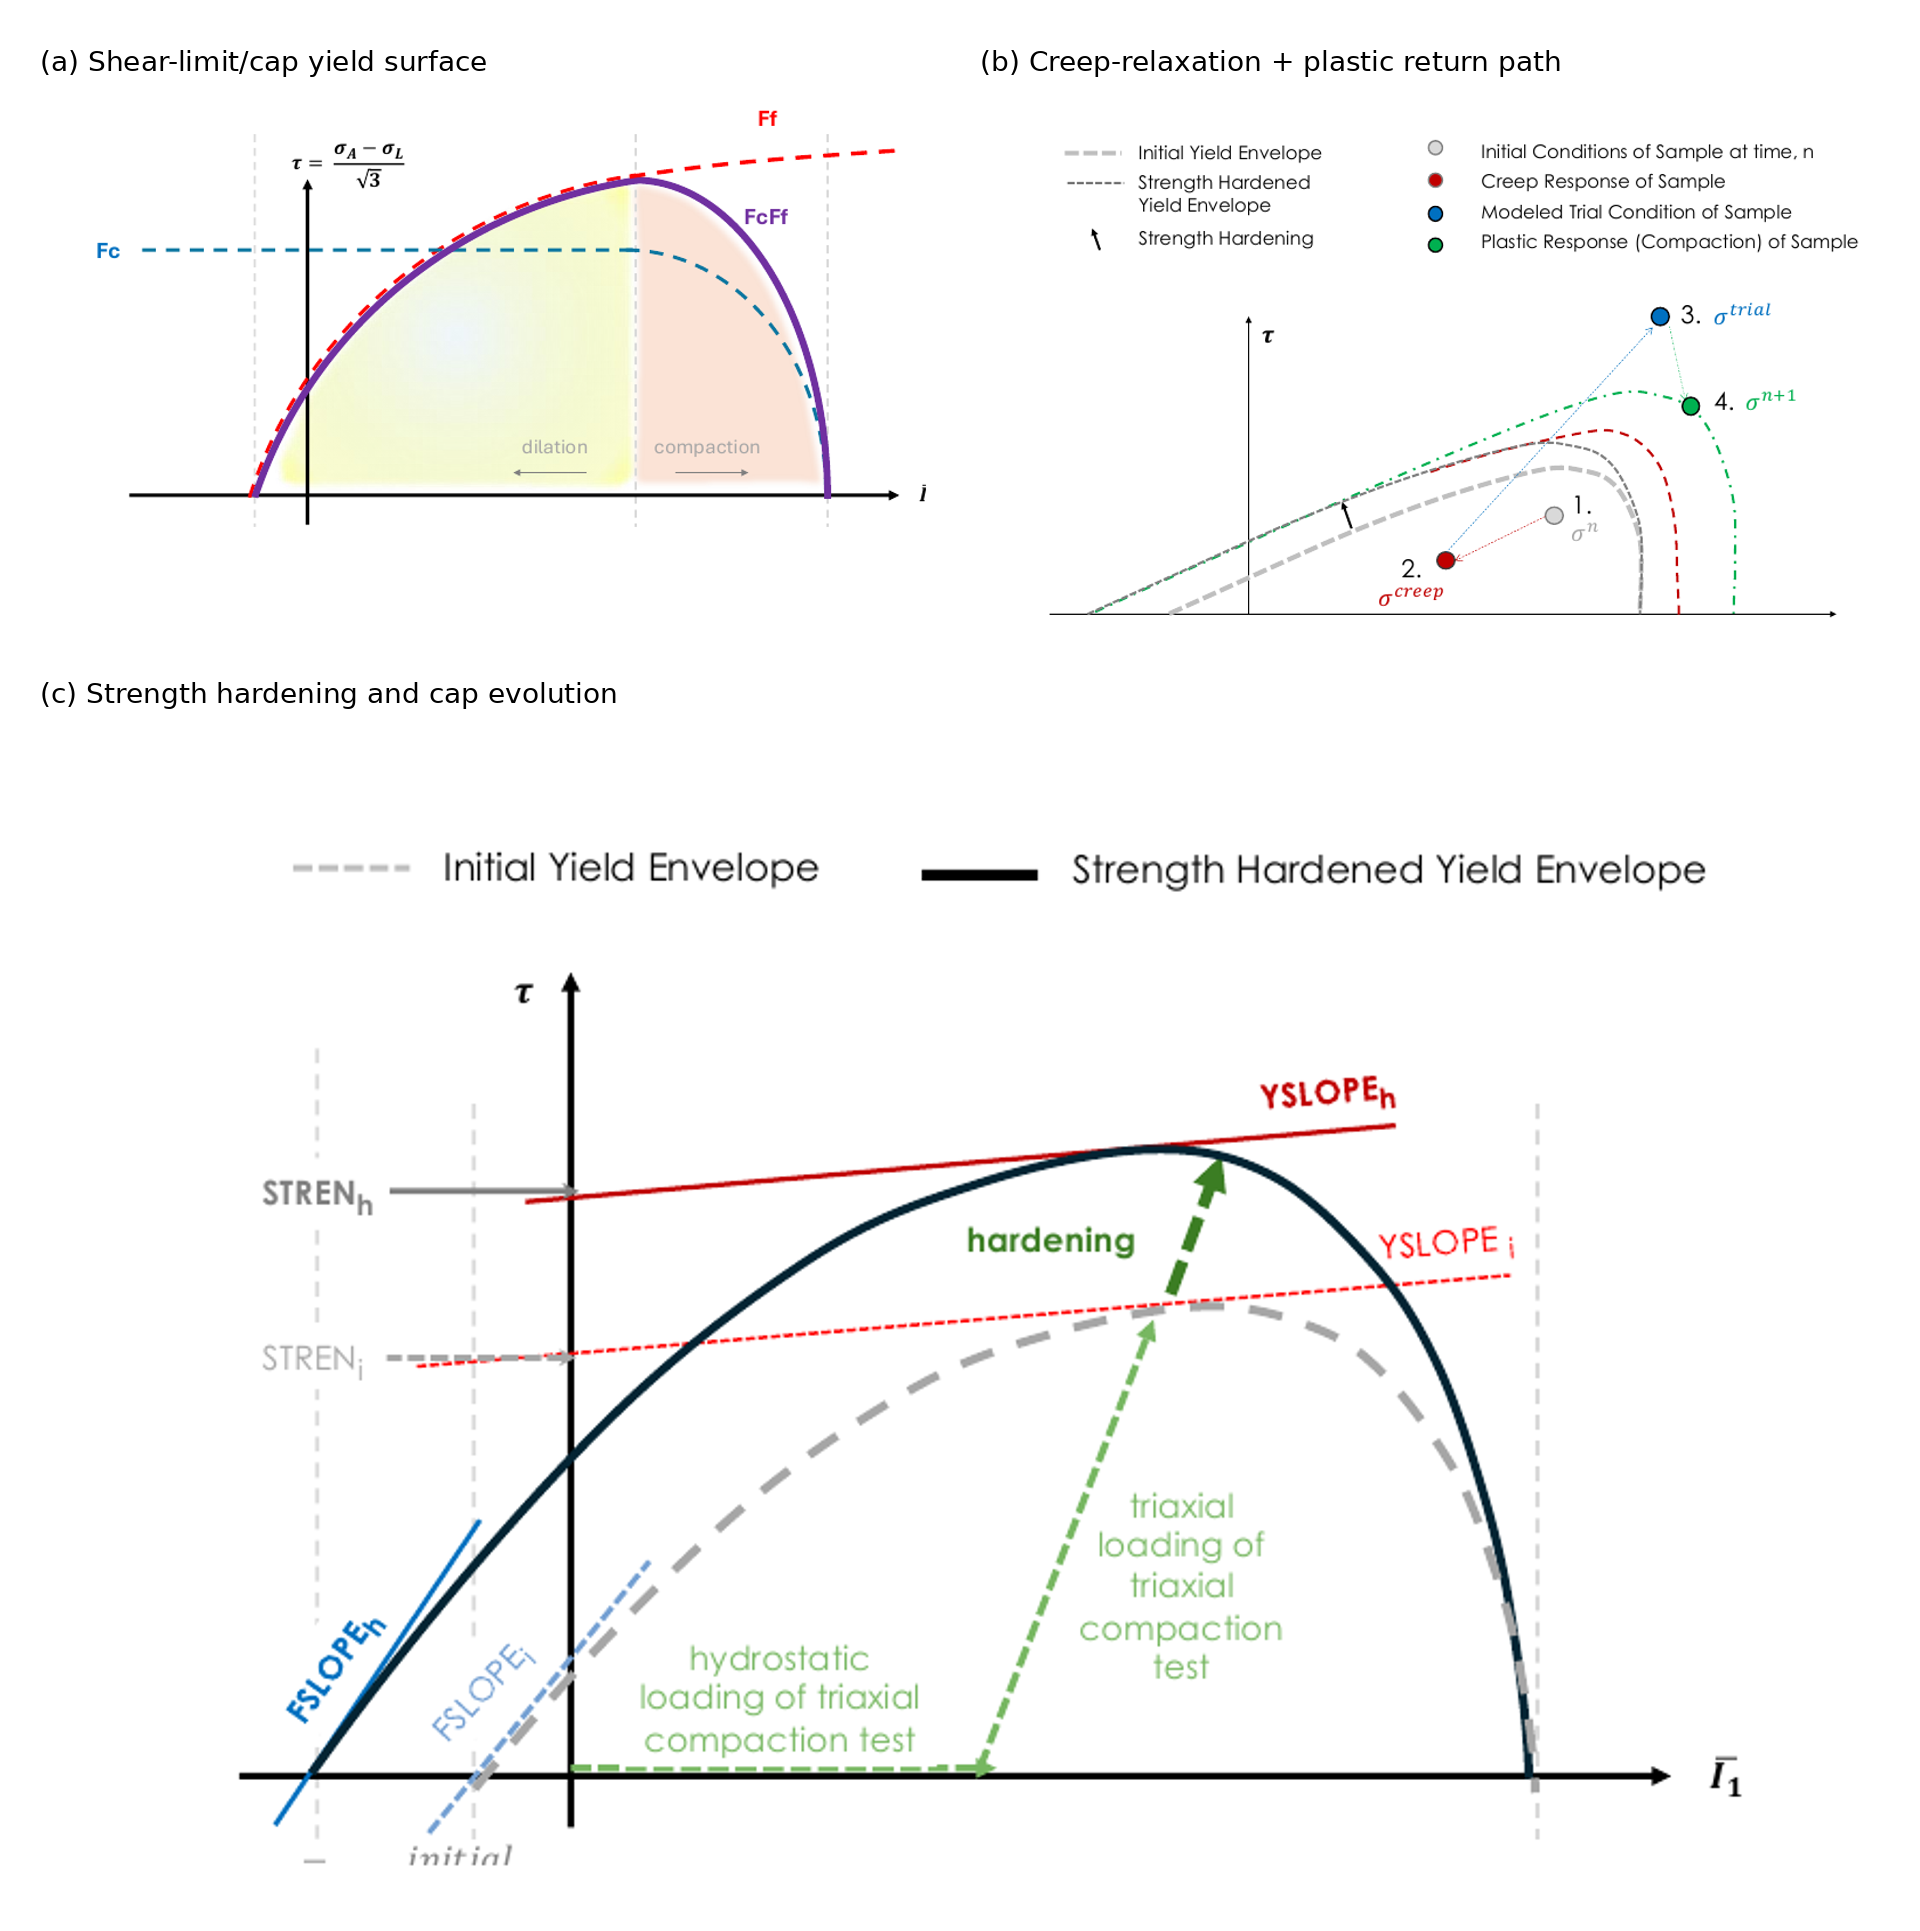
\includegraphics[width=0.98\linewidth]{figures/geomechanics_formulation_composite.png}
  \caption{Geomechanics formulation diagrams adapted from Malenda, Homel, Kibikas, Choens, Shalev, and Lyakhovsky~\cite{malenda2025ghareb}.  (a) The shear-limit function is multiplied by a cap function to obtain a pressure-sensitive strength surface.  (b) Creep first relaxes the beginning-of-step state, then an elastic trial stress is computed, and a plastic return is performed to the evolved surface.  (c) Strain hardening expands the strength envelope and shifts the triaxial-loading response.}
  \label{fig:geomechanics-formulation}
\end{figure}

\paragraph{Supported shear-limit parameterizations.}
The same input fields can represent several useful pressure-dependent limits.  The host-side input checks enforce a valid combination.
\begin{longtable}{@{}p{0.24\linewidth}p{0.68\linewidth}@{}}
\caption{Shear-limit surface families selected by \texttt{Geomechanics} inputs.\label{tab:geomechanics-surface-families}}\\
\toprule
\textbf{Family} & \textbf{Input pattern and purpose}\\
\midrule
\endfirsthead
\toprule
\textbf{Family} & \textbf{Input pattern and purpose}\\
\midrule
\endhead
Linear Drucker--Prager & \texttt{fSlope > 0}, \texttt{peakI1 >= 0}, and \texttt{stren = ySlope = 0}.  This gives a linear pressure-dependent shear limit.\\
Von Mises & \texttt{stren > 0} with \texttt{fSlope = peakI1 = ySlope = 0}.  This gives pressure-independent shear strength.\\
Zero-vertex transition & \texttt{fSlope > 0}, \texttt{stren > 0}, and \texttt{peakI1 = ySlope = 0}.  This connects a zero-pressure vertex to a finite shear plateau.\\
Nonlinear Drucker--Prager & \texttt{fSlope > ySlope > 0}, \texttt{stren > ySlope*peakI1}, and \texttt{peakI1 >= 0}.  This is the full curved form used for many geomaterial fits.\\
\bottomrule
\end{longtable}

For the nonlinear branch, the code computes
\begin{align}
  a_1 &= \texttt{STREN}_h, \\
  a_2 &= \frac{\texttt{FSLOPE}_h-\texttt{YSLOPE}_h}{\texttt{STREN}_h-\texttt{YSLOPE}_h\,\texttt{PEAKI1}_h},\\
  a_3 &= \left(\texttt{STREN}_h-\texttt{YSLOPE}_h\,\texttt{PEAKI1}_h\right)
         \exp\left[-a_2\,\texttt{PEAKI1}_h\right],\\
  a_4 &= \texttt{YSLOPE}_h.
  \label{eq:geomechanics-limit-parameters}
\end{align}
The linear and special-case surfaces are obtained by setting the corresponding subset of \(a_i\) to zero, as described in Table~\ref{tab:geomechanics-surface-families}.

\paragraph{Nonlinear elasticity.}
The tangent bulk modulus is evaluated from the beginning-of-substep stress and volumetric plastic strain.  In the dry path used by the reviewed code,
\begin{equation}
  K = b_0 + b_1\exp\left(\frac{b_2}{I_1}\right) - b_3\exp\left(\frac{b_4}{\epsilon_v^p}\right),
  \qquad I_1<0, \quad \epsilon_v^p<0,
  \label{eq:geomechanics-bulk-modulus}
\end{equation}
with lower bound \(K\ge b_0\).  The tensile/low-pressure response uses \(K=b_0\).  The shear modulus defaults to \(G=g_0\).  If \texttt{g1} is nonzero, the model computes a pressure-dependent Poisson ratio,
\begin{equation}
  \nu = g_1 + g_2\exp\left(\frac{g_3}{I_1}\right), \qquad 0\le \nu < \frac{1}{2},
  \label{eq:geomechanics-poisson}
\end{equation}
then sets
\begin{equation}
  G = \max\left[g_0,\frac{3K(1-2\nu)}{2(1+\nu)}\right].
  \label{eq:geomechanics-shear-modulus}
\end{equation}
This is a pragmatic pressure-dependent tangent stiffness for fitting laboratory data; it is evaluated substep-by-substep so the trial predictor follows the local tangent response.

\paragraph{Cap hardening, porosity, and crush curve.}
The cap position \(X\) is computed from volumetric plastic strain \(\epsilon_v^p=\operatorname{tr}\boldsymbol{\epsilon}^p\).  The implemented dry crush curve is
\begin{equation}
  X(\epsilon_v^p)=
  \begin{cases}
    \dfrac{p_0p_1+\ln\left[(\epsilon_v^p+p_3)/p_3\right]}{p_1}, & \epsilon_v^p\le 0,\\[0.8em]
    p_0(1+\epsilon_v^p)^{1/(p_0p_1p_3)}, & \epsilon_v^p>0,
  \end{cases}
  \label{eq:geomechanics-crush-curve}
\end{equation}
where \texttt{p0 < 0}, \texttt{p1 > 0}, and \texttt{p3 > 0}.  If \(\epsilon_v^p\) approaches \(-p_3\), the cap is pushed to a very large compressive value so the material behaves as fully compacted.  The particle porosity stored for plotting and subsequent material response is
\begin{equation}
  \phi = 1 + \exp(-\epsilon_v^p)(\phi_i-1),
  \qquad
  \phi_i = 1-\exp(-p_3).
  \label{eq:geomechanics-porosity}
\end{equation}
Thus the same input \texttt{p3} sets the limiting volumetric plastic compaction and the initial unloaded porosity implied by the crush curve.

\paragraph{Strain hardening and damage softening.}
The equivalent plastic shear strain is computed from the plastic-strain deviator.  When \texttt{strainHardeningK > 0}, the hardening increment is
\begin{equation}
  H = K_h\left(1-\exp[-n_h\,\bar\epsilon_p]\right),
  \label{eq:geomechanics-hardening}
\end{equation}
where \(K_h=\texttt{strainHardeningK}\) and \(n_h=\texttt{strainHardeningN}\).  The coherence \(c=1-D\) softens the surface through \(c^\psi\), where \(\psi=\texttt{fractureSofteningExponent}\).  In implementation form,
\begin{align}
  \texttt{STREN}_h &= b_{\mathrm{buckling}}\left(\texttt{stren}+H\,\texttt{dstrendh}\right),\\
  \texttt{FSLOPE}_h &= c^\psi\,\texttt{fSlope}\left(1+H\,\texttt{dfslopedh}\right)
  +\left(1-c^\psi\right)\texttt{fSlopeFailed},\\
  \texttt{PEAKI1}_h &= b_{\mathrm{buckling}}\left(\texttt{peakI1}+H\,\texttt{dpeakI1dh}\right)c^\psi s_p,\\
  c_{r,h} &= \operatorname{clamp}\left[\texttt{cr}\left(1+H\,\texttt{dcrdh}/g_0\right),10^{-10},0.99999999999\right],
  \label{eq:geomechanics-hardening-parameters}
\end{align}
where \(s_p\) is the particle \texttt{strengthScale}.  In this model, \texttt{strengthScale} is applied to the tensile-vertex/\texttt{peakI1} branch and to the fracture-stress threshold; it should not be assumed to scale every coefficient identically.  See Section~\ref{subsubsec:strength-scale-weibull} for the shared Weibull-strength discussion.

Damage is optional and active only when \texttt{fractureEnergyReleaseRate} is positive.  The model stores damage as \(D=1-c\).  Depending on \texttt{damageEvolutionCriterion}, damage increments are driven by dilatational plastic work or by a combined dilatational/shear plastic-work measure below a brittle--ductile transition pressure.  In schematic form,
\begin{equation}
  \Delta D = \frac{\Delta W_p\,\ell_{ch}}{G_f}, \qquad
  c^{n+1}=\max(0,c^n-\Delta D),
  \label{eq:geomechanics-damage}
\end{equation}
where \(G_f=\texttt{fractureEnergyReleaseRate}\) and \(\ell_{ch}\) is the particle length scale.  The damage threshold uses \texttt{fractureStress*strengthScale}; this is another model-specific use of \texttt{strengthScale}.  The \texttt{damageEvolutionCriterion=2} branch estimates the brittle--ductile transition from the apex of the current surface, while \texttt{damageEvolutionCriterion=1} uses the user-provided \texttt{brittleDuctileTransition}.

\paragraph{Optional creep relaxation.}
When \texttt{enableCreep=1}, creep is applied once over the full explicit time increment before the plastic substep retry loop.  The code uses an Arrhenius-like temperature multiplier
\begin{equation}
  A_T = \exp\left[-\frac{Q}{R}\left(\frac{1}{T}-\frac{1}{T_0}\right)\right],
  \label{eq:geomechanics-temperature-creep}
\end{equation}
where \(Q=\texttt{Q}\), \(T_0=\texttt{initialTemperature}\), and \(R\) is the gas constant.  Deviatoric creep uses an equilibrium plastic shear strain and relaxes the deviatoric stress toward it:
\begin{align}
  \gamma_{eq} &= C_0\,\tau^{C_1},\\
  \Delta\gamma_c &= \Delta t\,A_T C_2\max(\gamma_{eq}-\gamma_p,0),
  \label{eq:geomechanics-dev-creep}
\end{align}
with \(C_0=\texttt{creepC0}\), \(C_1=\texttt{creepC1}\), and \(C_2=\texttt{creepC2}\).  The increment is limited by the current elastic shear strain so creep cannot reverse the deviatoric stress in one step.

Volumetric creep uses the current unloaded porosity \(\phi_p\), an equilibrium porosity \(\phi_e\), and a pressure-dependent rate:
\begin{align}
  \phi_e &= \texttt{creepA}\exp\left[-\left(\frac{p}{\texttt{creepB}}\right)^{\texttt{creepD}}\right]
           + \texttt{creepE} - 0.0002\langle T-T_0\rangle - 3\times 10^{-6}\langle T-T_0\rangle^2,\\
  \frac{d\phi_p}{dt} &= -A_T\left(\frac{p}{\texttt{creepG}}\right)^{\texttt{creepF}}
  \texttt{creepC}\left(\phi_p-\phi_e\right),
  \label{eq:geomechanics-vol-creep}
\end{align}
where \(\langle x\rangle=\max(x,0)\).  The creep-updated porosity is converted back to an equivalent volumetric plastic strain and used to relax the beginning-of-step pressure.  As in the Ghareb-chalk implementation, the creep relaxation is intended to represent slow mechanisms in an explicit-dynamics calculation only when creep time scales are separated from elastic-wave and plastic-return time scales~\cite{malenda2025ghareb}.

\paragraph{Optional compaction/buckling multiplier.}
For porous or architected solids, \texttt{enableBuckling} applies a prescribed strength multiplier before the cap/plastic update.  With \texttt{enableBuckling=1}, the strain measure is volumetric, based on \(J=\det\mathbf{F}\).  With \texttt{enableBuckling=2}, the strain measure is directional, based on the stretch along \texttt{MaterialDirection}.  The multiplier has the form
\begin{equation}
  b_{\mathrm{buckling}} = 1-A_b\sin^2\left[-\left\lceil\frac{\ell_{ch}}{L_b}\right\rceil\pi\hat\epsilon\right],
  \label{eq:geomechanics-buckling}
\end{equation}
where \(A_b=\texttt{bucklingAmplitude}\), \(L_b=\texttt{bucklingLength}\), and \(\hat\epsilon\) is a normalized compaction strain.  This is an empirical multiplier, not a resolved structural-buckling analysis.

\paragraph{Numerical update algorithm.}
The GEOS-MPM call path is corotational.  The velocity gradient is unrotated into the beginning-of-step frame, symmetrized to form the strain-rate tensor, and the old plastic strain is also unrotated.  The model then performs the update in that frame and rotates the plastic strain back at the end of the step.

\begin{lstlisting}[caption={Geomechanics update structure.},label={alg:geomechanics-update},basicstyle=\ttfamily\small]
unrotate velocity gradient and plastic strain to beginning-of-step frame
D = sym(L_unrotated)
compute optional buckling multiplier from F and MaterialDirection
compute tangent K, G and conservative wave speed
if inelasticity is disabled:
  sigma = sigma_old + [3 K iso(D) + 2 G dev(D)] dt
else:
  estimate required substeps from trial stress and tangent-stiffness change
  apply optional full-step creep relaxation to sigma_old, ep_old, and X
  for progressively refined subcycle attempts:
    for each substep:
      evaluate K, G from current stress and plastic strain
      sigma_trial = hypoelastic predictor
      compute hardening, damage-modified surface coefficients, and yield state
      if elastic: accept trial state
      else:
        compute nonhardening return by transformed bisection/search
        if cap or backstress evolves:
          solve consistency on volumetric plastic strain by bounded bisection
        update plastic strain, cap X, coherence c, and porosity
    if all substeps succeed: accept attempt
  if all attempts fail: restore state and set constitutiveUpdateFlag = -1
rotate plastic strain back to end-of-step frame and store stress, damage, porosity
\end{lstlisting}

The nonhardening return uses the CB-TSCPR idea: transform the stress space so the energy-norm return becomes a Euclidean closest-point search, use bisection from an interior point to the trial point, and rotate the candidate point in transformed space until the closest boundary point is found~\cite{homel2015cbtscpr}.  The nonassociativity parameter \texttt{beta} enters this transformation by scaling the deviatoric coordinate,
\begin{equation}
  r^* = \beta\sqrt{\frac{3K}{2G}}\,r,
  \qquad r=\sqrt{2J_2},
  \label{eq:geomechanics-transformed-space}
\end{equation}
so the return direction can represent reduced or enhanced dilatation without constructing a separate flow-potential surface.  If the cap position changes with volumetric plastic strain, the solver wraps this return in a consistency bisection on \(\eta\in[0,1]\), where
\begin{equation}
  \Delta\epsilon_v^p = \eta\,\Delta\epsilon_{v,0}^p.
  \label{eq:geomechanics-consistency-eta}
\end{equation}
Each trial \(\eta\) updates \(X\), coherence, and the shifted-stress state, recomputes the return, and checks that the computed volumetric plastic strain matches the assumed value.  This decoupling is the main numerical reason the model can combine nonlinear elasticity, cap hardening, softening, and nonassociativity while retaining a robust update path.

\paragraph{Input parameterization.}
Table~\ref{tab:geomechanics-parameters} summarizes the major input groups.  The recommended calibration workflow is to fit \texttt{b0--b4} and \texttt{p0,p1,p3} from hydrostatic loading/unloading, fit \texttt{g0--g3}, \texttt{peakI1}, \texttt{fSlope}, \texttt{stren}, and \texttt{ySlope} from triaxial compression/extension data, then fit \texttt{strainHardeningK}, \texttt{strainHardeningN}, damage, and creep parameters from post-yield, dilation, compaction, and creep histories.

\begin{longtable}{@{}p{0.22\linewidth}p{0.28\linewidth}p{0.42\linewidth}@{}}
\caption{Main \texttt{Geomechanics} input groups.  See the generated schema appendix for the exact XML registration status and defaults.\label{tab:geomechanics-parameters}}\\
\toprule
\textbf{Group} & \textbf{Inputs} & \textbf{Role}\\
\midrule
\endfirsthead
\toprule
\textbf{Group} & \textbf{Inputs} & \textbf{Role}\\
\midrule
\endhead
Elasticity & \texttt{b0,b1,b2,b3,b4}, \texttt{g0,g1,g2,g3,g4} & Nonlinear tangent bulk modulus, pressure-dependent Poisson ratio, shear modulus, and conservative wave-speed estimate.  \texttt{g4} is registered but not active in the reviewed update path.\\
Cap/crush curve & \texttt{p0,p1,p2,p3,p4}, \texttt{cr} & Hydrostatic compaction curve, initial porosity relation, cap position, and cap branch point.  \texttt{p2} and \texttt{p4} are registered but currently unused.\\
Shear limit & \texttt{peakI1}, \texttt{fSlope}, \texttt{fSlopeFailed}, \texttt{stren}, \texttt{ySlope}, \texttt{beta} & Drucker--Prager/Kayenta-style shear surface, residual frictional slope, tensile vertex, and transformed-space nonassociativity.\\
Hardening & \texttt{strainHardeningK}, \texttt{strainHardeningN}, \texttt{dstrendh}, \texttt{dfslopedh}, \texttt{dpeakI1dh}, \texttt{dcrdh} & Exponential shear hardening and model-specific changes to strength, slope, tensile vertex, and cap branch.\\
Damage & \texttt{fractureEnergyReleaseRate}, \texttt{fractureSofteningExponent}, \texttt{fractureStress}, \texttt{brittleDuctileTransition}, \texttt{damageEvolutionCriterion} & Optional work-regularized reduction of coherence, with either user-specified or internally estimated brittle--ductile transition.\\
Creep and temperature & \texttt{enableCreep}, \texttt{creepC0}, \texttt{creepC1}, \texttt{creepC2}, \texttt{creepA}, \texttt{creepB}, \texttt{creepC}, \texttt{creepD}, \texttt{creepE}, \texttt{creepF}, \texttt{creepG}, \texttt{initialTemperature}, \texttt{Q} & Optional volumetric and deviatoric creep relaxation and temperature-scaled rates.\\
Buckling multiplier & \texttt{enableBuckling}, \texttt{bucklingLength}, \texttt{bucklingAmplitude}, \texttt{MaterialDirection} & Optional empirical compaction multiplier using volumetric or directional strain.\\
Numerical controls & \texttt{plasticStrainTolerance}, \texttt{stressReturnTolerance}, \texttt{maxAllowedSubcycles}, \texttt{failedStepResponse}, \texttt{disableInelasticity} & Return tolerances, subcycling limits, failure response, and elastic-only test mode.  Failed convergence exposes \texttt{constitutiveUpdateFlag=-1} to the solver robustness/deletion path.\\
Currently disabled fluid path & \texttt{fluidBulkModulus}, \texttt{fluidInitialPressure} & Must be zero in the reviewed implementation.  The code retains placeholders for a future persistent pore-pressure/backstress state.\\
\bottomrule
\end{longtable}

\paragraph{Implementation notes.}
The model writes \texttt{bulkModulus}, \texttt{shearModulus}, \texttt{porosity}, \texttt{damage}, \texttt{temperature}, and \texttt{constitutiveUpdateFlag} fields.  The stored \texttt{porosity} is an evolving continuum porosity inferred from volumetric plastic strain, not merely a visualization flag.  The stored \texttt{constitutiveUpdateFlag} is zero for normal updates, may be one when the model needed additional subcycling, and is set to \(-1\) when the update fails and the solver should treat the particle through the robustness/deletion logic in Section~\ref{sec:robustness-controls}.  The implementation is presently a dry porous solid model with optional empirical creep; coupled heat transfer, active fluid pressure, and fully coupled pore-pressure/backstress evolution are future extensions rather than active input options.


\subsection{Fluid models}
\label{subsec:fluid-constitutive-models}
\index{constitutiveModels!fluid models}

The reviewed MPM continuum dispatch includes a gas-like continuum model.  The PFW and XML infrastructure can assign this model to particles in the same way as solid models, but its stress is purely spherical.  A future liquid model can use the same dispatch path once implemented.

\subsubsection{\texttt{Gas}}
\label{subsubsec:gas-model}
\index{constitutiveModels!Gas}
\index{gas model}

\texttt{Gas} is a simple ideal-gas-style pressure model.  It computes a pressure from the reference pressure, the deformation-gradient Jacobian, and a temperature ratio, then returns a spherical compressive stress:
\begin{equation}
  p = \frac{p_0}{J}\frac{T}{T_0},
  \qquad
  \boldsymbol{\sigma}=-p\mathbf{I}.
  \label{eq:gas-pressure}
\end{equation}
The wave speed is evaluated as
\begin{equation}
  c = \sqrt{\gamma p/\rho},
  \qquad \gamma=1.4
  \label{eq:gas-wavespeed}
\end{equation}
for the current implementation.

\begin{lstlisting}[caption={Gas stress update.},label={alg:gas-update},basicstyle=\ttfamily\small]
pressure = referencePressure / jacobian * (temperature / referenceTemperature)
stress = -pressure * I
waveSpeed = sqrt(1.4 * pressure / density)
\end{lstlisting}

The gas model has special handling in the robustness/deformation-gradient-reset path (Section~\ref{sec:robustness-controls}) because a gas particle does not require the same persistent deviatoric deformation history as a solid particle.

\subsubsection{Liquid-model placeholder}
\label{subsubsec:liquid-model-placeholder}
\index{constitutiveModels!liquid placeholder}

A liquid-particle model is not currently documented as an active MPM continuum model in the reviewed snapshot.  A future liquid model could be introduced through the same material dispatch interface, for example with a weakly compressible equation of state,
\begin{equation}
  p = p_0 + K_f\left(\frac{\rho}{\rho_0}-1\right),
  \qquad
  \boldsymbol{\sigma}=-p\mathbf{I}+2\eta\operatorname{dev}\mathbf{D},
  \label{eq:liquid-placeholder}
\end{equation}
where \(K_f\) is a fluid bulk modulus and \(\eta\) is a dynamic viscosity.  This equation is a design placeholder only; it should not be interpreted as an implemented input option until a concrete GEOS-MPM liquid model is registered and verified.

\subsection{Shared constitutive modifiers and particle state}
\label{subsec:constitutive-modifiers}
\index{constitutive modifiers}

Several particle fields are not full constitutive models, but they modify how one or more models evaluate strength, damage, heat, or anisotropy.  These fields may be painted by geometry wrappers in PFW, updated by solver events, or updated by a constitutive model.  Because the same field may be interpreted differently by different models, this section documents the common data path and the expected modeling interpretation; model-specific equations should be added to the detailed material subsections before quantitative calibration.

\subsubsection{Strength scale and Weibull-type size effects}
\label{subsubsec:strength-scale-weibull}
\index{strengthScale}
\index{Weibull statistics}
\index{constitutive modifiers!strengthScale}

The particle field \texttt{strengthScale} is a multiplicative scalar that can be assigned by PFW geometry wrappers such as \texttt{strengthScaleWrapper} and by Voronoi/layered Weibull wrappers.  Models that expose a \texttt{strengthScale} wrapper then read the value during the constitutive update.  In brittle materials this field is often used to represent flaw-controlled size effects or mesoscopic heterogeneity.

A common theoretical basis is Weibull weakest-link scaling~\cite{weibull1951}.  For a reference volume \(V_0\), reference strength \(\sigma_0\), and Weibull modulus \(m\), the failure probability of a uniformly stressed volume \(V\) is often written
\begin{equation}
  P_f = 1 - \exp\left[-\frac{V}{V_0}\left(\frac{\sigma}{\sigma_0}\right)^m\right].
  \label{eq:weibull-failure-probability}
\end{equation}
At fixed failure probability this gives the familiar deterministic size scaling
\begin{equation}
  \sigma(V) = \sigma_0\left(\frac{V_0}{V}\right)^{1/m}.
  \label{eq:weibull-size-scaling}
\end{equation}
A stochastic PFW wrapper may instead sample a flaw population and assign a particle-level scale factor \(s_p\) so that the material model evaluates a local strength such as \(Y_p=s_pY_0\) or \(\sigma_{f,p}=s_p\sigma_f\).  The exact placement of \(s_p\) is model dependent: for example, some models multiply tensile and compressive strengths, some multiply fracture-energy parameters only when an option is enabled, and some models do not use the field at all.  For that reason, \texttt{strengthScale} should be documented in each detailed material subsection before it is used for quantitative calibration.

\subsubsection{Crack-tip stress concentration}
\label{subsubsec:crack-tip-stress-concentration}
\index{crack-tip stress concentration}
\index{distanceToCrackTip}
\index{constitutive modifiers!crack-tip correction}

The crack-tip correction is a solver/constitutive coupling used by damage models that need an unresolved stress-concentration estimate near a DFG fracture tip, motivated by the Griffith-Irwin crack-tip picture~\cite{griffith1921,irwin1957}.  The solver first uses the neighbor-list damage field to compute a nonlocal damage gradient and a local Hessian-like diagnostic.  Particles that satisfy the tip-detection threshold receive a positive \texttt{distanceToCrackTip}; other particles receive zero.  Models such as \texttt{CeramicDamage} and \texttt{Graphite} can then compute and store a plotted \texttt{crackTipStressConcentration} factor.

The current correction has the form
\begin{equation}
  C_{\mathrm{tip}}
  = \max\left(1,\sqrt{\frac{d_{\mathrm{tip}}}{r_{\mathrm{fpz}}}}\right),
  \label{eq:crack-tip-stress-concentration-outline}
\end{equation}
where \(d_{\mathrm{tip}}\) is the inverse-kernel estimate of the unresolved distance to the crack tip and \(r_{\mathrm{fpz}}\) is a process-zone length constructed from fracture toughness or fracture energy and a nominal intact strength.  The intent is to avoid over-predicting the resolved particle strength when the MPM/DFG length scale cannot resolve the near-tip stress field.  The correction is optional and should be verified against the intended fracture model and neighbor radius.

\subsubsection{Porosity}
\label{subsubsec:constitutive-porosity}
\index{porosity}
\index{constitutive modifiers!porosity}

\texttt{porosity} is a particle field that may be initialized by PFW, painted by wrappers such as \texttt{porosityWrapper} or \texttt{pointwisePorosityWrapper}, read by a constitutive model, and in some models updated as part of the material response.  In the reviewed code path, porous/damage models use porosity differently.  For example, \texttt{Geomechanics} carries porosity as an evolving material variable, while \texttt{CeramicDamage} uses porosity in strength scaling.  Solver events and future coupled solvers may also modify porosity, for example to represent healing, compaction, reaction, or pore closure.

Because porosity can be both an input descriptor and a constitutive state variable, users should distinguish the initial particle field from any model-updated value written after the first constitutive step.  Future coupled heat/fluid/chemistry or poromechanics updates should document ownership rules: whether the solver, a flow model, or the solid constitutive model is the authoritative updater for \texttt{porosity} at a given step.

\subsubsection{Temperature}
\label{subsubsec:constitutive-temperature}
\index{temperature}
\index{constitutive modifiers!temperature}
\index{TemperatureProfile event}
\index{TemperatureRamp event}

\texttt{temperature} and \texttt{temperatureRate} are particle fields shared by the solver, events, and thermally sensitive constitutive models.  PFW can initialize temperature through geometry wrappers, while events such as \texttt{TemperatureProfile} can prescribe domain-wide histories from an event-local table.  The reviewed code also records internal energy and includes constitutive hooks for temperature-dependent parameters.  Models such as \texttt{StrainHardeningPolymer}, \texttt{Graphite}, and \texttt{Geomechanics} read temperature-dependent terms; other models may ignore temperature unless later extended.

In a purely mechanical run, temperature may be prescribed externally or inferred internally by a constitutive model from plastic work, strain energy, or an equation of state.  In future coupled runs, a heat-transfer solver could become the authoritative updater.  Until those ownership rules are formalized for a given application, input files should make clear whether temperature is a fixed initial condition, an event-prescribed history, a material-model output, or a field reserved for later coupling.

\subsection{External material models}
\label{subsec:external-material-models}
\index{constitutiveModels!external material models}
\index{external material models}
\index{setupMPM!external material models}

GEOS-MPM can compile continuum material models that live outside the public source tree.  This path is intended for site-local, application-specific, or proprietary continuum laws without requiring those files to be committed to the main repository.  The build hook is the CMake cache variable \texttt{GEOS\_EXTERNAL\_CONSTITUTIVE\_MODELS\_DIR}; the \texttt{setupMPM} helper described in Section~\ref{sec:setupMPM} forwards this path through the option \texttt{--external-material-models}.

A minimal external material-model directory has the form
\begin{lstlisting}[caption={Minimal external material-model directory layout.},label={lst:external-material-layout},basicstyle=\ttfamily\small]
my_external_materials/
  GEOSExternalConstitutiveModels.cmake
  MyContinuumModel.hpp
  MyContinuumModel.cpp
\end{lstlisting}
The manifest can also be named \texttt{CMakeLists.txt}.  For an explicit MPM continuum model, the manifest must list the source/header files and must also add the model type and include to the MPM dispatch lists:
\begin{lstlisting}[caption={External continuum model CMake registration.},label={lst:external-material-cmake},basicstyle=\ttfamily\small]
geos_register_external_constitutive_models(
  BASE_DIR ${CMAKE_CURRENT_LIST_DIR}
  SOURCES
    MyContinuumModel.cpp
  HEADERS
    MyContinuumModel.hpp
  MPM_INCLUDES
    MyContinuumModel.hpp
  MPM_MODELS
    MyContinuumModel )
\end{lstlisting}
The implementation file must still register the model with the normal GEOS constitutive catalog, for example
\begin{lstlisting}[language=C++,caption={External model GEOS catalog registration.},label={lst:external-material-catalog},basicstyle=\ttfamily\small]
REGISTER_CATALOG_ENTRY( ConstitutiveBase,
                        MyContinuumModel,
                        std::string const &,
                        Group * const )
\end{lstlisting}
After the files are in place, configure and build using either the setup helper or a direct CMake configuration:
\begin{lstlisting}[language=bash,caption={Building with external continuum material models.},label={lst:external-material-build},basicstyle=\ttfamily\small]
./setupMPM --dane --external-material-models /path/to/my_external_materials

# Equivalent direct-CMake idea:
cmake -DGEOS_EXTERNAL_CONSTITUTIVE_MODELS_DIR=/path/to/my_external_materials ...
cmake --build <build-dir> --target geosx
\end{lstlisting}

Once built, the external material is used like any other continuum model: add a corresponding XML tag to the \texttt{Constitutive} block, add its name to the relevant \texttt{ParticleRegion} material list, and assign the matching material index with PFW geometry objects or wrappers.  External cohesive-zone laws use a related but separate registration list and are documented with the cohesive-zone infrastructure in Section~\ref{sec:cohesive-zone-implementation}.


\section{Particle types and interpolation/update options}
\label{sec:particle-types-and-mapping}
\index{particle types}
\index{particle mapping}
\index{CPDI}
\index{B-spline}
\index{PIC}
\index{FLIP}
\index{XPIC}
\index{FMPM}

This section documents the interpolation and particle update choices used by the MPM solver.  The user-facing particle-type controls are generated by ParticleFileWriter and are summarized with the other material, group, and particle-type controls in Section~\ref{sec:pfw-materials}; this section focuses on the internal numerical operators.  The reviewed code exposes the particle-type enumeration
\begin{equation}
  \texttt{SinglePoint},\quad
  \texttt{SinglePointBSpline},\quad
  \texttt{CPDI},\quad
  \texttt{CPTI},\quad
  \texttt{CPDI2},
\end{equation}
and the velocity/state update enumeration
\begin{equation}
  \texttt{FLIP},\quad \texttt{PIC},\quad \texttt{XPIC},\quad \texttt{FMPM}.
\end{equation}
The implemented particle setup paths in the reviewed source are \texttt{SinglePoint}, \texttt{SinglePointBSpline}, and \texttt{CPDI}.  The \texttt{CPTI} and \texttt{CPDI2} identifiers are reserved for future development; attempting to generate those particle types in the reviewed particle setup path raises a not-implemented error.  The same particle-to-grid and grid-to-particle mapping data are reused by the force, kinematic, contact, boundary, and diagnostic steps described in Sections~\ref{sec:solver-steps} and~\ref{sec:bc-internals}.

\subsection{Mapping notation and effective support}
\label{subsec:mapping-notation}
\index{particle mapping!notation}

Let $p$ denote a material point, $I$ a background-grid node, $m_p$ the particle mass, $V_p$ the particle volume, $\boldsymbol{x}_p$ the particle position, $\boldsymbol{v}_p$ the particle velocity, and $\boldsymbol{\sigma}_p$ the Cauchy stress.  The solver stores, for each active particle, a sparse set of mapped nodes together with shape values $N_{Ip}$ and gradients $\boldsymbol{\nabla}N_{Ip}$.  These quantities define the standard MPM projections
\begin{align}
  m_I &= \sum_p m_p N_{Ip},
  &
  \boldsymbol{p}_I &= \sum_p m_p \boldsymbol{v}_p N_{Ip},
  &
  \boldsymbol{v}_I &= \frac{\boldsymbol{p}_I}{m_I},
  \label{eq:mpm-p2g-mass-momentum}\\
  \boldsymbol{f}^{\mathrm{int}}_I
    &= -\sum_p V_p\,\boldsymbol{\sigma}_p\boldsymbol{\nabla}N_{Ip},
  &
  \boldsymbol{L}_p
    &= \sum_I \boldsymbol{v}_I\otimes \boldsymbol{\nabla}N_{Ip},
  \label{eq:mpm-p2g-force-gradient}
\end{align}
with additional material-field or group labels used when contact and boundary branches need split nodal states.  Equations~\eqref{eq:mpm-p2g-mass-momentum} and~\eqref{eq:mpm-p2g-force-gradient} are the common PIC/FLIP MPM transfer operators introduced for solid mechanics by Sulsky, Chen, and Schreyer and later generalized through GIMP, CPDI, and related domain methods \cite{sulsky1994history,sulsky1995solid,bardenhagen2004gimp,sadeghirad2011cpdi}.

The implementation distinguishes a raw geometric support from an effective support.  For \texttt{SinglePoint}, the raw map has the eight trilinear nodes of the cell containing the particle.  For \texttt{SinglePointBSpline}, the raw map has the $4^3=64$ tensor-product cubic B-spline control nodes surrounding the particle.  For \texttt{CPDI}, each of the eight particle-domain corners contributes eight trilinear nodes, again giving as many as 64 raw entries.  A coalescing pass combines repeated grid nodes, sums their contributions, removes zero entries, and provides the effective map used by most particle-to-grid and grid-to-particle kernels.  This detail matters because CPDI corners may share grid nodes after distortion or near grid boundaries, and because B-spline support is broader than linear MPM support even though it is still driven by a single particle center.

\subsection{Single-point particles with trilinear mapping}
\label{subsec:single-point-linear}
\index{SinglePoint}
\index{particle mapping!single point}

The \texttt{SinglePoint} type is the classical point-quadrature MPM discretization.  The particle characteristic function is a Dirac measure located at $\boldsymbol{x}_p$, and the background basis is the trilinear finite-element basis on the cell containing the particle.  If $\boldsymbol{h}=(h_x,h_y,h_z)$ is the local cell spacing and
\begin{equation}
  \boldsymbol{s}=(s_x,s_y,s_z),
  \qquad
  s_d=\frac{x_{p,d}-x_{0,d}}{h_d}\in[0,1],
  \label{eq:single-point-local-coord}
\end{equation}
are the local coordinates measured from the lower cell corner, then the one-dimensional linear weights are
\begin{equation}
  \ell_0(s)=1-s,
  \qquad
  \ell_1(s)=s,
  \qquad
  \frac{d\ell_0}{dx}=-\frac{1}{h},
  \qquad
  \frac{d\ell_1}{dx}=\frac{1}{h}.
  \label{eq:linear-mpm-weights}
\end{equation}
For a node with local index $\boldsymbol{a}=(a_x,a_y,a_z)$, $a_d\in\{0,1\}$,
\begin{align}
  N_{\boldsymbol{a}p}
    &= \ell_{a_x}(s_x)\ell_{a_y}(s_y)\ell_{a_z}(s_z),
  \label{eq:linear-mpm-shape}\\
  \frac{\partial N_{\boldsymbol{a}p}}{\partial x}
    &= \frac{d\ell_{a_x}}{dx}(s_x)\ell_{a_y}(s_y)\ell_{a_z}(s_z),
  \label{eq:linear-mpm-grad-x}
\end{align}
with cyclic permutations for $y$ and $z$.  The weights satisfy partition of unity and reproduce linear fields inside a cell, but the gradient is discontinuous at cell boundaries.  Consequently, standard point MPM is susceptible to cell-crossing noise and quadrature error when particles move from one background cell to another.  These errors motivated the generalized interpolation material point method, smoother basis studies, CPDI, and related projection improvements \cite{bardenhagen2004gimp,steffen2008quadrature,steffen2008choices,wallstedt2007projection}.

In the reviewed implementation the \texttt{SinglePoint} generator stores a volume and visualization domain vectors, but the interpolation itself uses only the particle center.  The stored domain vectors allow the particle file and plotting tools to display a finite volume, while the map used by Equations~\eqref{eq:mpm-p2g-mass-momentum}--\eqref{eq:mpm-p2g-force-gradient} remains the eight-node point map in Equation~\eqref{eq:linear-mpm-shape}.

\subsection{Single-point particles with cubic B-spline mapping}
\label{subsec:single-point-bspline}
\index{SinglePointBSpline}
\index{B-spline!cubic}
\index{particle mapping!B-spline}

The \texttt{SinglePointBSpline} type keeps the particle as a point quadrature rule but replaces the trilinear cell basis by a tensor-product cubic cardinal B-spline basis.  The support is four nodes in each direction, giving $64$ grid nodes in three dimensions.  Let
\begin{equation}
  u_d = \frac{x_{p,d}-x^{\min}_d}{h_d},
  \qquad
  i_d=\lfloor u_d\rfloor,
  \qquad
  s_d=u_d-i_d\in[0,1),
\end{equation}
and let the first supported node in direction $d$ be $i_d-1$.  For one dimension, the four nonzero cubic B-spline weights used by the solver are
\begin{align}
  b_0(s) &= \frac{(1-s)^3}{6},
  &
  b_1(s) &= \frac{3s^3-6s^2+4}{6},
  \label{eq:bspline-cubic-weights-a}\\
  b_2(s) &= \frac{-3s^3+3s^2+3s+1}{6},
  &
  b_3(s) &= \frac{s^3}{6}.
  \label{eq:bspline-cubic-weights-b}
\end{align}
Their derivatives with respect to physical position are
\begin{align}
  \frac{db_0}{dx} &= -\frac{(1-s)^2}{2h},
  &
  \frac{db_1}{dx} &= \frac{1.5s^2-2s}{h},
  \label{eq:bspline-cubic-grads-a}\\
  \frac{db_2}{dx} &= \frac{-1.5s^2+s+0.5}{h},
  &
  \frac{db_3}{dx} &= \frac{s^2}{2h}.
  \label{eq:bspline-cubic-grads-b}
\end{align}
The three-dimensional basis is the tensor product
\begin{equation}
  N_{\boldsymbol{a}p}=b_{a_x}(s_x)b_{a_y}(s_y)b_{a_z}(s_z),
  \qquad
  a_d\in\{0,1,2,3\},
  \label{eq:bspline-tensor-product}
\end{equation}
and the gradient is obtained by differentiating the one-dimensional factor in the selected coordinate direction.  The code applies a deterministic closure correction to the final supported node so that the sum of the stored shape values is exactly one and the sum of the stored gradients is exactly zero to roundoff.

The motivation for this option is the same as in smoother-basis MPM studies: broader, smoother basis functions reduce force and velocity projection jumps when particles cross grid-cell boundaries.  Steffen et al. analyzed implementation choices and quadrature errors in MPM, and later B-spline MPM work showed that B-spline bases can reduce cell-crossing artifacts and improve continuity of grid fields \cite{steffen2008quadrature,steffen2008choices,gan2018bspline}.  The GEOS option should be interpreted as a single-point B-spline quadrature choice, not as a finite particle-domain method: the particle center controls the interpolation, while the stored particle domain vectors are retained for volume accounting and output.

\begin{figure}[tbp]
  \centering
  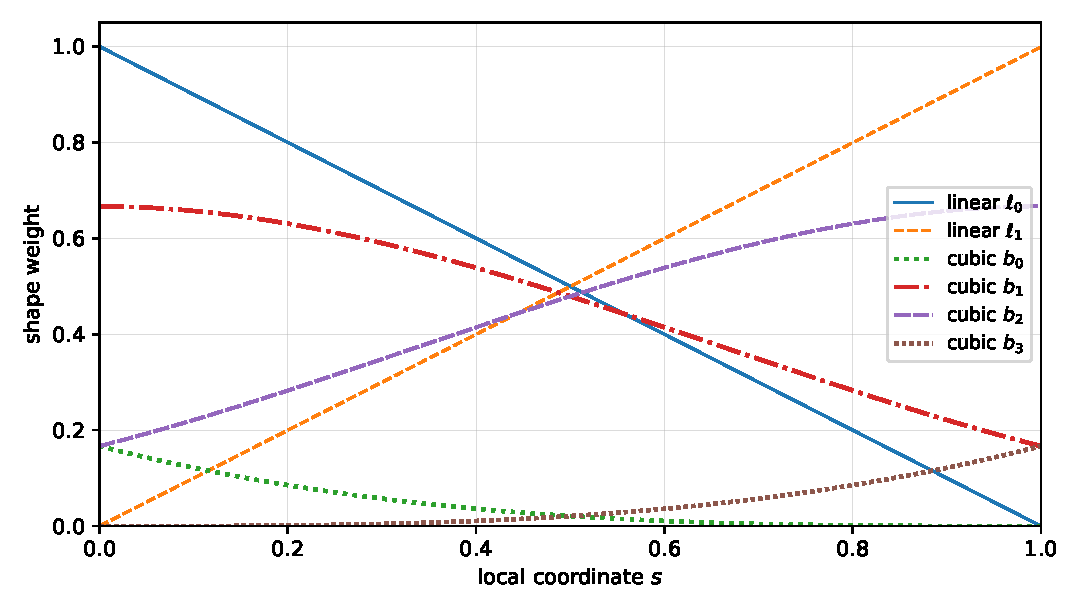
\includegraphics[width=0.92\linewidth]{figures/particle_shape_functions.pdf}
  \caption{One-dimensional shape functions used to build the tensor-product maps.  The linear MPM map has two active weights on the host cell, whereas the cubic B-spline map has four active weights with $C^2$ continuity across cell interfaces.  The three-dimensional maps are tensor products of these one-dimensional functions.}
  \label{fig:particle-shape-functions}
\end{figure}

\begin{lstlisting}[caption={Single-point cubic B-spline map construction.},basicstyle=\ttfamily\small]
for each active particle p:
  for d in x,y,z:
    u = (x_p[d] - grid_min[d]) / h[d]
    cell = floor(u)
    s = u - cell
    base[d] = cell - 1
    compute b[0:4](s) and dbdx[0:4](s)
  for a,b,c in 0..3:
    I = node(base[x]+a, base[y]+b, base[z]+c)
    N_Ip = bx[a] * by[b] * bz[c]
    gradN_Ip = (dbx[a]*by[b]*bz[c],
                 bx[a]*dby[b]*bz[c],
                 bx[a]*by[b]*dbz[c])
  adjust last entry so sum(N)=1 and sum(gradN)=0
\end{lstlisting}

\subsection{CPDI with trilinear background shape functions}
\label{subsec:cpdi-linear}
\index{CPDI}
\index{particle domain}
\index{particle mapping!CPDI}

The \texttt{CPDI} type implements convected particle domain interpolation for a parallelepiped particle domain.  CPDI replaces point evaluation of the grid basis by a particle-domain average, thereby reducing cell-crossing noise and improving behavior under large deformation.  This follows the convected particle domain interpolation method of Sadeghirad, Brannon, and Burghardt \cite{sadeghirad2011cpdi}.  In GEOS, the particle carries a center $\boldsymbol{x}_p$ and three half-edge vectors $\boldsymbol{r}_1$, $\boldsymbol{r}_2$, and $\boldsymbol{r}_3$.  The current domain is
\begin{equation}
  \Omega_p = \left\{
  \boldsymbol{x}_p+\xi_1\boldsymbol{r}_1+
  \xi_2\boldsymbol{r}_2+
  \xi_3\boldsymbol{r}_3
  \;:\;
  -1\le \xi_1,\xi_2,\xi_3\le 1
  \right\},
  \label{eq:cpdi-domain}
\end{equation}
with volume
\begin{equation}
  V_p = 8\,\boldsymbol{r}_1\cdot(\boldsymbol{r}_2\times\boldsymbol{r}_3).
  \label{eq:cpdi-volume}
\end{equation}
For the eight corners $c$, define signs $s^c_i\in\{-1,1\}$ and corner positions
\begin{equation}
  \boldsymbol{x}^c_p = \boldsymbol{x}_p
   +s^c_1\boldsymbol{r}_1+s^c_2\boldsymbol{r}_2+s^c_3\boldsymbol{r}_3.
  \label{eq:cpdi-corners}
\end{equation}
The GEOS map evaluates the background trilinear shape functions at each corner and assigns one-eighth of the corner contribution to the particle map,
\begin{equation}
  \overline{N}_{Ip}
  \approx \frac{1}{8}\sum_{c=1}^{8} N_I(\boldsymbol{x}^c_p).
  \label{eq:cpdi-shape-average}
\end{equation}
For gradients, let
\begin{equation}
  \boldsymbol{A}=\boldsymbol{r}_2\times\boldsymbol{r}_3,
  \qquad
  \boldsymbol{B}=\boldsymbol{r}_3\times\boldsymbol{r}_1,
  \qquad
  \boldsymbol{C}=\boldsymbol{r}_1\times\boldsymbol{r}_2.
  \label{eq:cpdi-area-vectors}
\end{equation}
The corner gradient coefficient used internally is
\begin{equation}
  \boldsymbol{\alpha}^c_p
  =\frac{s^c_1\boldsymbol{A}+s^c_2\boldsymbol{B}+s^c_3\boldsymbol{C}}{V_p},
  \label{eq:cpdi-alpha}
\end{equation}
and the effective gradient is assembled as
\begin{equation}
  \boldsymbol{\nabla}\overline{N}_{Ip}
  \approx \sum_{c=1}^{8} N_I(\boldsymbol{x}^c_p)\,\boldsymbol{\alpha}^c_p.
  \label{eq:cpdi-gradient-average}
\end{equation}
Equations~\eqref{eq:cpdi-shape-average}--\eqref{eq:cpdi-gradient-average} are stored initially as corner/node raw entries and then coalesced by grid node.  A closure adjustment enforces the corner partition of unity and gradient consistency before the raw entries are merged.

\begin{lstlisting}[caption={CPDI map construction for a parallelepiped particle domain.},basicstyle=\ttfamily\small]
for each active CPDI particle p:
  A = r2 x r3; B = r3 x r1; C = r1 x r2
  V = 8 * dot(r1,A)
  for each corner sign sc in {-1,1}^3:
    x_c = x_p + sc[0]*r1 + sc[1]*r2 + sc[2]*r3
    alpha_c = (sc[0]*A + sc[1]*B + sc[2]*C) / V
    evaluate eight trilinear grid weights N_I(x_c)
    for each corner node I:
      raw_N_Ip     += (1/8) * N_I(x_c)
      raw_grad_Ip  += alpha_c * N_I(x_c)
  coalesce duplicate nodes and enforce consistency corrections
\end{lstlisting}

CPDI remains a background-grid method: nodal equations are still solved on the rectilinear grid, but the particle basis carries an evolving domain.  The particle domain vectors are updated by the deformation history, and the volume used in the stress divergence reflects the convected domain.  This is especially important for large tensile strains and rotations, where point MPM may develop severe quadrature error or numerical fracture.  The domain-averaged CPDI map trades a larger stencil for smoother transfer and a more physically meaningful particle support \cite{sadeghirad2011cpdi,homel2016domaindef}.

\subsection{CPDI domain scaling}
\label{subsec:cpdi-domain-scaling}
\index{CPDI!domain scaling}
\index{domain scaling}
\index{numerical fracture}

The code includes an optional CPDI domain-scaling procedure.  The intent is to limit excessive growth of convected domains relative to the background grid, which can otherwise delay localization, smear gradients, or contribute to numerical fracture in parallel CPDI calculations.  The relevant literature basis is the CPDI domain-scaling work of Homel, Brannon, and Guilkey \cite{homel2016domaindef}.

The reviewed implementation constructs diagonal-like vectors from the current half-edge vectors and caps their lengths by
\begin{equation}
  \ell_{\mathrm{crit}} = 0.49999\min_d h_d,
  \label{eq:cpdi-domain-scale-lcrit}
\end{equation}
where $h_d$ are the current grid spacings.  In plane-strain calculations the two controlled vectors are
\begin{equation}
  \boldsymbol{\ell}_0=\boldsymbol{r}_1+\boldsymbol{r}_2,
  \qquad
  \boldsymbol{\ell}_1=\boldsymbol{r}_1-\boldsymbol{r}_2.
  \label{eq:cpdi-scaling-2d-lvectors}
\end{equation}
If $\|\boldsymbol{\ell}_i\|>\ell_{\mathrm{crit}}$, the vector is scaled to length $\ell_{\mathrm{crit}}$ and the half-edge vectors are reconstructed as
\begin{equation}
  \boldsymbol{r}_1=\frac{1}{2}(\boldsymbol{\ell}_0+\boldsymbol{\ell}_1),
  \qquad
  \boldsymbol{r}_2=\frac{1}{2}(\boldsymbol{\ell}_0-\boldsymbol{\ell}_1).
  \label{eq:cpdi-scaling-2d-reconstruct}
\end{equation}
In three dimensions the four controlled body diagonals are
\begin{align}
  \boldsymbol{\ell}_0&=\boldsymbol{r}_1+\boldsymbol{r}_2+\boldsymbol{r}_3,
  &
  \boldsymbol{\ell}_1&=\boldsymbol{r}_1-\boldsymbol{r}_2+\boldsymbol{r}_3,
  \label{eq:cpdi-scaling-3d-lvectors-a}\\
  \boldsymbol{\ell}_2&=\boldsymbol{r}_2-\boldsymbol{r}_1+\boldsymbol{r}_3,
  &
  \boldsymbol{\ell}_3&=\boldsymbol{r}_3-\boldsymbol{r}_1-\boldsymbol{r}_2.
  \label{eq:cpdi-scaling-3d-lvectors-b}
\end{align}
After applying the same length cap, the half-edge vectors are reconstructed as
\begin{align}
  \boldsymbol{r}_1&=\frac{1}{4}(\boldsymbol{\ell}_0+\boldsymbol{\ell}_1-\boldsymbol{\ell}_2-\boldsymbol{\ell}_3),
  &
  \boldsymbol{r}_2&=\frac{1}{4}(\boldsymbol{\ell}_0-\boldsymbol{\ell}_1+\boldsymbol{\ell}_2-\boldsymbol{\ell}_3),
  \label{eq:cpdi-scaling-3d-reconstruct-a}\\
  \boldsymbol{r}_3&=\frac{1}{4}(\boldsymbol{\ell}_0+\boldsymbol{\ell}_1+\boldsymbol{\ell}_2+\boldsymbol{\ell}_3).
  \label{eq:cpdi-scaling-3d-reconstruct-b}
\end{align}
A particle flag records that scaling occurred.  If requested by input options, the solver can still plot unscaled domains by reconstructing the current vectors from the reference vectors and deformation gradient.  A separate guard disables surface normals and surface positions for highly distorted, scaled particles when the aspect-ratio threshold used by the code is exceeded.  Thus, domain scaling is not a new constitutive model; it is a numerical regularization of the CPDI interpolation domain before subsequent mapping and output operations.

\subsection{CPTI and CPDI2 placeholders}
\label{subsec:cpti-cpdi2-placeholders}
\index{CPTI}
\index{CPDI2}

The \texttt{CPTI} and \texttt{CPDI2} particle-type names are present in the enumeration but are not implemented in the reviewed particle-generation path.  They are retained in this manual as forward links to the methods intended by those names.

\paragraph{CPTI.}
Convected-particle tetrahedron interpolation represents the particle domain by tetrahedra rather than by a parallelepiped.  The method was introduced for mesoscale ceramic calculations by Leavy, Guilkey, Phung, Spear, and Brannon and was motivated by the need to represent complex material geometry while retaining the efficiency of a rectilinear computational grid \cite{leavy2019cpti}.  A future GEOS implementation would need particle-domain storage for tetrahedral vertices, tetrahedral volume and face-gradient rules, particle-to-grid support construction for each convected tetrahedron, and output conventions for deformed tetrahedral domains.

\paragraph{CPDI2.}
Second-order CPDI generalizes the original CPDI parallelogram/parallelepiped representation to more flexible quadrilateral or hexahedral particle domains and supports enrichment for weak discontinuities at material interfaces \cite{sadeghirad2013cpdi2}.  In the code snapshot reviewed for this manual, the \texttt{CPDI2} generator branch is a placeholder.  Completing it would require storage for the full convected hexahedral geometry, generalized corner or quadrature-gradient weights, robust coalescing for larger supports, and consistency tests against the published CPDI2 patch and interface examples.

\subsection{Transfer operators used by update schemes}
\label{subsec:update-transfer-operators}
\index{particle update}
\index{grid-to-particle transfer}

The update schemes can be described compactly by two transfer operators.  Let $S$ denote the particle-to-grid velocity projection
\begin{equation}
  (S\boldsymbol{v})_I = \frac{1}{m_I}\sum_p m_p N_{Ip}\boldsymbol{v}_p,
  \label{eq:operator-S}
\end{equation}
and let $S^+$ denote the grid-to-particle interpolation
\begin{equation}
  (S^+\boldsymbol{v})_p = \sum_I N_{Ip}\boldsymbol{v}_I.
  \label{eq:operator-S-plus}
\end{equation}
With lumped nodal mass, $S^+$ is an interpolation operator rather than an exact inverse of $S$.  Much of the behavior of PIC, FLIP, XPIC, and FMPM follows from how much filtering is introduced by repeated application of these operators.  PIC applies a direct grid velocity interpolation, FLIP updates particles by the grid acceleration increment, XPIC builds higher-order filters from repeated projections, and FMPM approximates the action of a full mass matrix inverse.  The projection accuracy and stability consequences of such choices have been studied by Wallstedt and Guilkey, Hammerquist and Nairn, and Nairn and Hammerquist \cite{wallstedt2007projection,wallstedt2008explicit,hammerquist2017xpic,nairn2021fmpm}.

\subsection{PIC update}
\label{subsec:pic-update}
\index{PIC}
\index{particle update!PIC}

The \texttt{PIC} option updates particle velocities by interpolating the current post-force, post-contact grid velocity.  In a conventional notation,
\begin{align}
  \boldsymbol{v}^{n+1}_p
    &= \sum_I N_{Ip}\boldsymbol{v}^{n+1}_I,
  \label{eq:pic-velocity}\\
  \boldsymbol{x}^{n+1}_p
    &= \boldsymbol{x}^{n}_p
     +\Delta t\sum_I N_{Ip}\left(\boldsymbol{v}^{n+1}_I
       -\frac{1}{2}\Delta t\,\boldsymbol{a}^{n+1}_I\right),
  \label{eq:pic-position}\\
  \boldsymbol{L}^{n+1}_p
    &= \sum_I \boldsymbol{v}^{n+1}_I\otimes\boldsymbol{\nabla}N_{Ip}.
  \label{eq:pic-velocity-gradient}
\end{align}
The position update in Equation~\eqref{eq:pic-position} is the time-centered form used by the reviewed implementation, in which the nodal acceleration term shifts the post-force velocity back to a midpoint-like transport velocity.  The velocity gradient used for stress integration is formed from the same grid velocity and the particle map gradients.

PIC is robust because the projection $S^+$ filters particle velocities through the grid every step, damping grid-scale null modes.  The cost of that filtering is numerical diffusion, especially in problems with persistent shear, impact, or oscillatory motion.  This tradeoff is the classical motivation for FLIP and for later XPIC filters: PIC damps noise effectively, while FLIP better preserves particle kinetic energy and history variables \cite{sulsky1995solid,brackbill1988flip,hammerquist2017xpic}.

\begin{lstlisting}[caption={PIC grid-to-particle update.},basicstyle=\ttfamily\small]
for each particle p:
  x_inc = 0; v_new = 0; L = 0
  for each mapped node I:
    x_inc += N_Ip * (v_I - 0.5*dt*a_I)
    v_new += N_Ip * v_I
    L     += outer(v_I, gradN_Ip)
  x_p += dt * x_inc
  v_p  = v_new
  L_p  = L
\end{lstlisting}

\subsection{FLIP update}
\label{subsec:flip-update}
\index{FLIP}
\index{particle update!FLIP}

The default \texttt{FLIP} option updates particle velocities by the nodal acceleration increment while transporting particles with the same time-centered grid velocity used in PIC:
\begin{align}
  \boldsymbol{v}^{n+1}_p
    &= \boldsymbol{v}^{n}_p
     +\Delta t\sum_I N_{Ip}\boldsymbol{a}^{n+1}_I,
  \label{eq:flip-velocity}\\
  \boldsymbol{x}^{n+1}_p
    &= \boldsymbol{x}^{n}_p
     +\Delta t\sum_I N_{Ip}\left(\boldsymbol{v}^{n+1}_I
       -\frac{1}{2}\Delta t\,\boldsymbol{a}^{n+1}_I\right),
  \label{eq:flip-position}\\
  \boldsymbol{L}^{n+1}_p
    &= \sum_I \boldsymbol{v}^{n+1}_I\otimes\boldsymbol{\nabla}N_{Ip}.
  \label{eq:flip-velocity-gradient}
\end{align}
Because FLIP increments the particle velocity rather than replacing it by $S^+\boldsymbol{v}_I$, it is much less diffusive than PIC.  This is important for dynamic solid mechanics, where over-filtering can erase physically meaningful velocity fluctuations or wave content.  The same property can also allow nonphysical particle-grid null-space noise to persist, particularly when particle distributions are irregular or contacts introduce sharp local changes.  The stability and accuracy of FLIP-like MPM updates depend strongly on particle density, projection quality, and the chosen particle basis \cite{brackbill1988flip,sulsky1995solid,wallstedt2007projection,wallstedt2008explicit}.

In the reviewed implementation, FLIP, PIC, and several diagnostic branches share the same effective mapping arrays.  For CPU execution, the code uses the coalesced map to avoid repeated grid-node contributions.  For device execution, some kernels can recompute or use raw support entries depending on the mapped-field and contact requirements.  These implementation choices do not change Equations~\eqref{eq:flip-velocity}--\eqref{eq:flip-velocity-gradient}; they only control how the sparse sums are evaluated.

\begin{lstlisting}[caption={FLIP grid-to-particle update.},basicstyle=\ttfamily\small]
for each particle p:
  x_inc = 0; dv = 0; L = 0
  for each mapped node I:
    x_inc += N_Ip * (v_I - 0.5*dt*a_I)
    dv    += N_Ip * a_I
    L     += outer(v_I, gradN_Ip)
  x_p += dt * x_inc
  v_p += dt * dv
  L_p  = L
\end{lstlisting}

\subsection{XPIC update}
\label{subsec:xpic-update}
\index{XPIC}
\index{particle update!XPIC}

The \texttt{XPIC} option implements the extended PIC method of Hammerquist and Nairn \cite{hammerquist2017xpic}.  XPIC introduces an update order $m$ that controls the degree of projection filtering.  At $m=1$, XPIC reduces to PIC.  Higher orders apply repeated particle-grid-particle projections in a way that damps the nonphysical null-space modes associated with under-resolved particle distributions without applying as much physical diffusion as PIC.  In the limit discussed by Hammerquist and Nairn, the method approaches a modified FLIP behavior while retaining improved stability.

The reviewed GEOS implementation builds XPIC corrections on the grid.  It initializes a pre-acceleration velocity-like field
\begin{equation}
  \boldsymbol{v}^{-}_I = \boldsymbol{v}^{n+1}_I-\Delta t\,\boldsymbol{a}^{n+1}_I,
  \label{eq:xpic-vminus}
\end{equation}
then repeatedly gathers this field to particles and scatters it back to the grid through the same shape functions and lumped masses used by the rest of the solver.  For each order index $r=2,\ldots,m$, the implementation uses coefficients
\begin{equation}
  c_r=\frac{m-r+1}{r},
  \qquad
  d_r=\frac{m-r}{r},
  \qquad
  \epsilon_r=(-1)^r,
  \label{eq:xpic-coefficients}
\end{equation}
for the velocity and velocity-difference projection terms.  The accumulated filtered grid field is then gathered to particles for the final velocity and position update.  The velocity gradient used for stress integration remains based on the physical post-force/contact grid velocity rather than on a separately filtered XPIC velocity gradient; this follows the implementation note in the reviewed solver and avoids introducing a second, inconsistent kinematic field.

\begin{lstlisting}[caption={XPIC update structure.},basicstyle=\ttfamily\small]
vMinus_I = v_I - dt*a_I
vStar_I  = 0
for r = 2..updateOrder:
  c  = (updateOrder - r + 1) / r
  dc = (updateOrder - r) / r
  gather vMinus_I to particles using N_Ip
  scatter projected particle field back to grid with m_p*N_Ip/m_I
  vStar_I += (-1)^r * projected_v_I
  vMinus_I = projected_v_I
for each particle p:
  gather the XPIC-filtered combination to update x_p and v_p
  L_p = sum_I outer(v_I, gradN_Ip)
\end{lstlisting}

XPIC is therefore best understood as a controllable compromise between PIC and FLIP.  It is appropriate when a calculation is too noisy with FLIP but too diffusive with PIC.  The practical input parameter is the update order, exposed as \texttt{updateOrder}; Section~\ref{sec:pfw-solver-controls} describes how this control is passed through ParticleFileWriter.

\subsection{FMPM update}
\label{subsec:fmpm-update}
\index{FMPM}
\index{full mass matrix}
\index{particle update!FMPM}

The \texttt{FMPM} option implements an approximate full-mass-matrix update based on the method of Nairn and Hammerquist \cite{nairn2021fmpm}.  Standard explicit MPM forms a lumped nodal mass $m_I$ and uses $m_I^{-1}$ in the nodal momentum equation.  Lumped mass is simple and robust, but it introduces numerical dissipation and projection errors because the true consistent mass matrix has off-diagonal coupling between grid basis functions.  FMPM constructs an iterative approximation to the action of the inverse full mass matrix while preserving the particle/grid data structures used by MPM.  The current documentation describes the solver in the incremental-correction interpretation of Nairn's 2026 implementation paper, in which each FMPM loop pass represents the velocity increment $\Delta v^{(\ell)}=v^{+(\ell)}-v^{+(\ell-1)}$ and lumped-mass features are imposed on that increment rather than only on the final filtered velocity \cite{nairn2026fmpm}.

At the operator level, FMPM applies a sequence involving $S$ and $S^+$.  The implementation initializes the cumulative FMPM grid velocity with the constrained post-contact grid velocity and then repeatedly projects the previous increment to particles and back to the grid.  Each iteration forms a residual-like increment and adds it to the cumulative velocity.  Homogeneous boundary constraints are applied to the increment so that constrained components do not re-enter through the higher-order correction.  Multi-field material-contact corrections are accumulated consistently as net contact momentum using the incremental contact correction described by Nairn \cite{nairn2026fmpm}.  The important distinction is that FMPM is intended to work with multi-field contact and with prescribed or moving grid-velocity boundary conditions; the limitation in the reviewed code snapshot is narrower, namely that the specific \texttt{boundaryConditionTypes == Contact} wall/contact-boundary bctype remains guarded and should be treated as untested until that branch is validated.

\begin{lstlisting}[caption={FMPM approximate full-mass update.},basicstyle=\ttfamily\small]
vFmpm_I = v_I
vPrev_I = v_I
for k = 2..updateOrder:
  gather vPrev_I to particles using N_Ip
  scatter gathered particle velocity back to grid with m_p*N_Ip/m_I
  vProj_I = projected grid velocity
  vPrev_I = vPrev_I - vProj_I
  apply homogeneous moving/symmetry boundary constraints to vPrev_I
  apply incremental multi-field material-contact correction if active
  vFmpm_I += vPrev_I
for each particle p:
  v_new = sum_I N_Ip * vFmpm_I
  x_p += 0.5*dt*(v_old + v_new)
  L_p  = sum_I outer(vFmpm_I, gradN_Ip)
  v_p  = v_new
\end{lstlisting}

Compared with FLIP, FMPM is designed to reduce dissipation associated with lumped-mass projection while retaining an explicit MPM structure.  The update order controls how many terms of the approximate inverse are retained.  Higher order can improve accuracy but increases cost because each additional term requires another gather/scatter synchronization and another round of boundary/contact consistency operations.  For production use, FMPM should be verified with the intended particle basis, contact model, and boundary configuration.  In particular, moving velocity boundary conditions and multi-field material contact use the incremental correction path, whereas the contact-wall boundary bctype should remain a separately tracked verification item.

\subsection{Implementation status summary}
\label{subsec:particle-update-status}
\index{particle types!implementation status}

Table~\ref{tab:particle-update-status} summarizes the status of the particle types and update schemes in the reviewed source snapshot.  The table is intended as a code-synchronized checklist for future documentation updates.

\begin{longtable}{p{0.25\linewidth}p{0.18\linewidth}p{0.48\linewidth}}
\caption{Particle mapping and update status in the reviewed source.}\label{tab:particle-update-status}\\
\toprule
Name & Status & Internal interpretation \\
\midrule
\endfirsthead
\toprule
Name & Status & Internal interpretation \\
\midrule
\endhead
\bottomrule
\endfoot
\texttt{SinglePoint} & implemented & Point particle with eight-node trilinear support.  Stored domain vectors are used for volume/output, not for interpolation. \\
\texttt{SinglePointBSpline} & implemented & Point particle with $4^3$ cubic B-spline support.  The center controls interpolation; domain vectors are retained for output/volume. \\
\texttt{CPDI} & implemented & Convected parallelepiped domain with corner-based trilinear integration, gradient coefficients from particle-domain area vectors, and optional domain scaling. \\
\texttt{CPTI} & placeholder & Reserved for convected tetrahedral particle domains; generator branch is not implemented in the reviewed source. \\
\texttt{CPDI2} & placeholder & Reserved for second-order CPDI with generalized hexahedral/quadrilateral domains; generator branch is not implemented in the reviewed source. \\
\texttt{PIC} & implemented & Replaces particle velocity by interpolated post-force grid velocity; robust but diffusive. \\
\texttt{FLIP} & implemented, default & Increments particle velocity by grid acceleration; less diffusive but can retain null-space noise. \\
\texttt{XPIC} & implemented & Higher-order PIC/FLIP compromise controlled by \texttt{updateOrder}; stress kinematics use physical grid velocity. \\
\texttt{FMPM} & implemented with restrictions & Approximate full-mass inverse controlled by \texttt{updateOrder}; uses the incremental correction path for moving velocity boundaries and multi-field material contact, while the \texttt{Contact} wall-boundary bctype remains guarded/untested in the reviewed branch. \\
\end{longtable}


\section{Boundary conditions, prescribed deformation, and stress control}
\label{sec:bc-internals}
\index{boundary conditions}
\index{Ftable}
\index{stress control}
\index{reactionHistory}

This section describes what the MPM solver does internally when boundary and domain-control options are active.  It deliberately separates the numerical implementation from the user-facing input syntax.  The user-facing \texttt{pfw\_input} controls, including examples of \texttt{boundaryConditionTypes}, \texttt{fTable}, \texttt{bcTable}, transverse boundary velocities, stress control, and periodic flags, are summarized in Section~\ref{sec:pfw-boundary-controls}.  The code path described here is the one reached during Step~13 of the explicit solver update, after particle-to-grid projection, MPI synchronization, grid trial dynamics, and optional material-field contact; see Section~\ref{subsec:solver-step-13}.

\subsection{Face convention and nodal data used by the boundary update}
\label{subsec:bc-face-convention}
\index{boundary conditions!face order}

The solver stores one boundary type for each axis-aligned face of the background grid.  The face order is
\begin{equation}
  f=0,1,2,3,4,5
  \quad\leftrightarrow\quad
  x^-,x^+,y^-,y^+,z^-,z^+.
\end{equation}
For face $f$, the normal coordinate direction is
\begin{equation}
  d(f)=\left\lfloor \frac{f}{2}\right\rfloor,
  \qquad
  s(f)=f\bmod 2,
  \qquad
  \alpha_f=-1+2s(f),
  \qquad
  \mathbf{n}_f=\alpha_f\mathbf{e}_{d(f)}.
  \label{eq:bc-face-normal}
\end{equation}
The two remaining coordinate directions are used as tangential directions.  In the code these are computed as
\begin{equation}
  d_1=(d+1)\bmod 3,
  \qquad
  d_2=(d+2)\bmod 3.
\end{equation}

Boundary enforcement operates on grid multi-fields.  The field index distinguishes material/contact velocity fields, while the node index distinguishes ordinary grid nodes, boundary nodes, and buffer/ghost-like nodes used to support the interpolation stencil near a face.  The principal fields modified by the boundary code are the grid velocity $\mathbf{v}_{I\alpha}$, grid acceleration $\mathbf{a}_{I\alpha}$, and grid velocity increment $\Delta\mathbf{v}_{I\alpha}$ for node $I$ and velocity field $\alpha$.  The boundary update also reads nodal mass, internal force, center-of-volume, surface-position, surface-field-mass, and ghost-rank data when contact or reaction histories are active.

The boundary-node and buffer-node sets are stored in the node-set repository as \texttt{boundaryNodes} and \texttt{bufferNodes}.  For a face $f$, let $\mathcal{B}_f$ be its boundary nodes and $\mathcal{G}_f$ its buffer nodes.  Each buffer node $G\in\mathcal{G}_f$ is paired with an interior node $J(G)$ and, for moving faces, a boundary node $B(G)$ at the same tangential grid coordinates.  These pairings are reconstructed from the structured-grid \texttt{ijkMap} and the current grid spacing.  They provide the even/odd extensions needed by B-spline and other wide-stencil particle-grid transfers near a boundary.

\subsection{Boundary-type state and time-dependent boundary-type switching}
\label{subsec:bc-table-internals}
\index{boundary conditions!bcTable}
\index{bcTable}

The runtime boundary-type array is \texttt{m\_boundaryConditionTypes}.  If the input does not provide this array, it is initialized to six \texttt{Outflow} entries.  If it is provided, the solver requires exactly six integer entries and checks that each entry belongs to the boundary-condition enumeration in Table~\ref{tab:bc-types}.

\begin{table}[htbp]
\centering
\caption{MPM boundary-condition type enumeration used by \texttt{SolidMechanicsMPM}.}
\label{tab:bc-types}
\begin{tabularx}{\linewidth}{@{}c l X@{}}
\toprule
Integer & Name & Internal interpretation \\
\midrule
0 & \texttt{Outflow} & Leave grid velocity and acceleration unconstrained on that face. \\
1 & \texttt{Symmetry} & Enforce zero normal velocity/acceleration and reflect buffer fields with an odd normal component and even tangential components. \\
2 & \texttt{Moving} & Enforce a prescribed affine normal velocity when prescribed boundary deformation or stress control is active; optionally enforce tangential velocities. \\
3 & \texttt{Contact} & Treat the face as a wall/contact plane.  Incoming nodes are corrected in the face-normal direction and optional boundary friction is applied in the tangential plane. \\
\bottomrule
\end{tabularx}
\end{table}

If \texttt{prescribedBcTable} is enabled, Step~4 of the explicit update calls \texttt{boundaryConditionUpdate} before particle-grid maps are assembled.  The table is a zero-order-hold schedule rather than an interpolated quantity.  For a time step beginning at $t^n$ with size $\Delta t$, the selected row is the last row whose time satisfies
\begin{equation}
  t_{\mathrm{row}} < t^n+\frac{\Delta t}{2}.
  \label{eq:bc-table-selection}
\end{equation}
The six boundary-type entries in that row then replace \texttt{m\_boundaryConditionTypes}.  After this update, \texttt{updateContactFlagsFromBoundaryConditions} sets \texttt{m\_hasContact} if either multiple velocity fields are present or at least one face is marked \texttt{Contact}.  This flag controls whether contact/surface fields are synchronized and whether contact-specific work is performed later in the step.

\begin{lstlisting}[caption={Boundary-type update and contact flag refresh.}]
if prescribedBcTable == 1:
  interval = last row i such that time_n + 0.5*dt > bcTable[i,0]
  for face in 0..5:
    boundaryConditionTypes[face] = bcTable[interval, face+1]

hasContact = (numVelocityFields > 1) or any(boundaryConditionTypes == Contact)
\end{lstlisting}

\subsection{Outflow faces}
\label{subsec:bc-outflow}
\index{boundary conditions!Outflow}

An \texttt{Outflow} face is the least intrusive boundary option.  In \texttt{applyEssentialBCs}, the face is skipped:
\begin{equation}
  \mathbf{v}_{I\alpha}^{\mathrm{after}}=\mathbf{v}_{I\alpha}^{\mathrm{before}},
  \qquad
  \mathbf{a}_{I\alpha}^{\mathrm{after}}=\mathbf{a}_{I\alpha}^{\mathrm{before}},
  \qquad I\in\mathcal{B}_f.
\end{equation}
No reflective buffer update is applied by the essential-boundary routine for this face.  This should not be interpreted as a finite-element natural traction boundary.  It means that the explicit MPM grid solve leaves the nodal values produced by particle-to-grid mapping, force assembly, contact, and MPI synchronization unchanged.  Particles that advect beyond a nonperiodic global domain are handled later by the out-of-range particle flagging and cleanup path.  Consequently, \texttt{Outflow} is useful for open-domain style calculations, impact problems where material may leave the computational box, or inactive directions in which the user does not want a symmetry or prescribed-motion constraint.

\subsection{Symmetry and free-slip reflection}
\label{subsec:bc-symmetry}
\index{boundary conditions!Symmetry}
\index{symmetry boundary conditions}

A \texttt{Symmetry} face enforces a kinematic free-slip plane.  On the boundary nodes, the normal component of the vector field is removed.  For velocity and acceleration this gives
\begin{equation}
  v_{I\alpha,d}=0,
  \qquad
  a_{I\alpha,d}=0,
  \qquad I\in\mathcal{B}_f.
  \label{eq:bc-symmetry-boundary-node}
\end{equation}
The corresponding velocity increment is updated so that XPIC/FMPM-style transfer formulas see the boundary-induced correction,
\begin{equation}
  \Delta v_{I\alpha,d} \leftarrow \Delta v_{I\alpha,d} - v_{I\alpha,d}^{\mathrm{old}}.
\end{equation}

For buffer nodes, the solver uses an odd extension of the normal component and an even extension of the tangential components from the interior paired node $J(G)$:
\begin{align}
  v_{G\alpha,d}   &= -v_{J(G)\alpha,d}, &
  v_{G\alpha,d_1} &=  v_{J(G)\alpha,d_1}, &
  v_{G\alpha,d_2} &=  v_{J(G)\alpha,d_2},
  \label{eq:bc-symmetry-buffer-velocity} \\
  a_{G\alpha,d}   &= -a_{J(G)\alpha,d}, &
  a_{G\alpha,d_1} &=  a_{J(G)\alpha,d_1}, &
  a_{G\alpha,d_2} &=  a_{J(G)\alpha,d_2}.
\end{align}
This mirrored extension is also applied earlier to mapped surface normals, center-of-mass vectors, and center-of-volume vectors on faces marked \texttt{Symmetry} or \texttt{Moving}.  That earlier pass occurs before the grid dynamics update and ensures that contact and surface quantities remain compatible with the same geometric reflection used for the final velocity and acceleration fields.

The construction is the MPM analogue of imposing an essential normal-velocity condition on the background grid while allowing tangential slip.  It is consistent with the grid-based enforcement commonly used in explicit MPM and GIMP calculations, where the particle state is advanced using constrained nodal accelerations and velocities rather than by imposing constraints directly on the particles \cite{sulsky1994history,bardenhagen2004gimp,wallstedt2008explicit}.

\begin{lstlisting}[caption={Symmetry-face enforcement.}]
for field alpha:
  for I in boundaryNodes[face]:
    dVelocity[I,alpha,d] = -velocity[I,alpha,d]
    velocity[I,alpha,d] = 0
    acceleration[I,alpha,d] = 0

  for G in bufferNodes[face]:
    J = reflected interior node for G
    velocity[G,alpha,d]  = -velocity[J,alpha,d]
    velocity[G,alpha,t1] =  velocity[J,alpha,t1]
    velocity[G,alpha,t2] =  velocity[J,alpha,t2]
    acceleration[G,alpha,d]  = -acceleration[J,alpha,d]
    acceleration[G,alpha,t1] =  acceleration[J,alpha,t1]
    acceleration[G,alpha,t2] =  acceleration[J,alpha,t2]
\end{lstlisting}

\subsection{Prescribed domain deformation and F-table interpolation}
\label{subsec:bc-ftable-internals}
\index{Ftable!interpolation}
\index{prescribedBoundaryFTable}
\index{prescribedFTable}

The F-table machinery produces a diagonal macroscopic deformation history and its associated diagonal velocity-gradient components.  The table has one time column and three deformation columns.  At the end of the step, $t^{n+1}=t^n+\Delta t$, \texttt{interpolateTable} evaluates the active interval and returns $F_i(t^{n+1})$ and $\dot F_i(t^{n+1})$.  For directions not completely overridden by stress control, the code sets
\begin{equation}
  \bar L_i(t^{n+1}) = \frac{\dot F_i(t^{n+1})}{F_i(t^{n+1})},
  \qquad
  \bar F_i(t^{n+1}) = F_i(t^{n+1}).
  \label{eq:bc-ftable-l}
\end{equation}
The current implementation supports three scalar interpolation kernels.  Let $y_0,y_1$ be consecutive table values, $\tau=(t^{n+1}-t_0)/(t_1-t_0)$, and $\Delta T=t_1-t_0$.  Linear interpolation uses
\begin{equation}
  y(\tau)=(1-\tau)y_0+\tau y_1,
  \qquad
  \dot y=\frac{y_1-y_0}{\Delta T}.
\end{equation}
Cosine interpolation uses
\begin{equation}
  y(\tau)=y_0-\frac{1}{2}(y_1-y_0)\left[\cos(\pi\tau)-1\right],
  \qquad
  \dot y=\frac{\pi}{2\Delta T}(y_1-y_0)\sin(\pi\tau),
\end{equation}
and \texttt{Smoothstep} uses the quintic polynomial
\begin{equation}
  y(\tau)=y_0+(y_1-y_0)(10\tau^3-15\tau^4+6\tau^5),
  \qquad
  \dot y=\frac{y_1-y_0}{\Delta T}(30\tau^2-60\tau^3+30\tau^4).
\end{equation}
Values before the first table time are clamped to the first row, and values after the final table time are clamped to the last row.

The two F-table flags route this macroscopic kinematics into different parts of the MPM update.  With \texttt{prescribedBoundaryFTable}, the diagonal velocity-gradient components become boundary velocities on \texttt{Moving} faces during \texttt{applyEssentialBCs}.  With \texttt{prescribedFTable}, the same components are superposed on particle velocity gradients and positions only in directions marked periodic by the spatial partition.  The latter path is intended for triply periodic or partially periodic homogeneous-deformation calculations.  In both cases, Step~18 later resizes the grid/domain measures using the current \texttt{domainL} values.

\subsection{Moving faces}
\label{subsec:bc-moving}
\index{boundary conditions!Moving}
\index{prescribedBoundaryTransverseVelocities}

A \texttt{Moving} face is an essential velocity boundary driven by the current domain velocity-gradient state.  In the reviewed implementation, the velocity constraint is applied only if either \texttt{prescribedBoundaryFTable} is active or at least one \texttt{stressControl} entry equals one.  This guard is important: marking a face as \texttt{Moving} without an active prescribed boundary deformation, or with only the limiting \texttt{stressControl} mode two active, does not by itself prescribe a nonzero velocity in \texttt{applyEssentialBCs}.

For a moving face $f$ normal to direction $d$, the code forms an end-of-step grid coordinate
\begin{equation}
  X_{I,d}^{n+1,*}=\left(1+\bar L_d\Delta t\right)X_{I,d}^{n},
\end{equation}
and imposes the normal velocity
\begin{equation}
  v_{I\alpha,d}^{\mathrm{bc}} = \bar L_d X_{I,d}^{n+1,*},
  \qquad I\in\mathcal{B}_f.
  \label{eq:bc-moving-normal-velocity}
\end{equation}
The solver then computes the increment and acceleration correction as
\begin{equation}
  \Delta v_{I\alpha,d} \leftarrow v_{I\alpha,d}^{\mathrm{bc}}-v_{I\alpha,d}^{\mathrm{old}},
  \qquad
  a_{I\alpha,d} \leftarrow a_{I\alpha,d}+\frac{v_{I\alpha,d}^{\mathrm{bc}}-v_{I\alpha,d}^{\mathrm{old}}}{\Delta t},
  \qquad
  v_{I\alpha,d}\leftarrow v_{I\alpha,d}^{\mathrm{bc}}.
  \label{eq:bc-moving-normal-correction}
\end{equation}

Tangential motion is optional.  If \texttt{enablePrescribedBoundaryTransverseVelocities[f]} is one, the two stored tangential values are enforced on $d_1$ and $d_2$ exactly as essential velocity components:
\begin{equation}
  v_{I\alpha,d_1}\leftarrow v_{f,d_1}^{\mathrm{presc}},
  \qquad
  v_{I\alpha,d_2}\leftarrow v_{f,d_2}^{\mathrm{presc}},
  \label{eq:bc-moving-transverse}
\end{equation}
with matching updates to \texttt{gridDVelocity} and \texttt{gridAcceleration}.  If transverse velocities are not enabled, the tangential components are left free on the boundary nodes.

The buffer-node extension is centered on the prescribed boundary value.  For the constrained normal component,
\begin{equation}
  v_{G\alpha,d}=-v_{J(G)\alpha,d}+2v_{B(G)\alpha,d}.
  \label{eq:bc-moving-buffer-normal}
\end{equation}
For tangential components, the code chooses either the same moving odd extension when transverse velocities are prescribed or a free-slip even extension otherwise:
\begin{equation}
  v_{G\alpha,d_k}=\begin{cases}
    -v_{J(G)\alpha,d_k}+2v_{B(G)\alpha,d_k}, & \text{prescribed transverse component active},\\
     v_{J(G)\alpha,d_k}, & \text{transverse component free},
  \end{cases}
  \qquad k=1,2.
  \label{eq:bc-moving-buffer-tangent}
\end{equation}
The same component-wise extension is applied to the acceleration.  This construction gives the interpolation stencil a boundary-consistent field: constrained components are odd about the prescribed control value, while unconstrained tangential components remain even.

\begin{lstlisting}[caption={Moving-face enforcement.}]
for field alpha and boundary node I:
  x_end = (1 + domainL[d]*dt) * gridPosition[I,d]
  v_bc = domainL[d] * x_end

  if transverse velocities enabled on this face:
    set velocity[I,alpha,t1] and velocity[I,alpha,t2]
    update dVelocity and acceleration corrections in t1,t2

  dVelocity[I,alpha,d] = v_bc - velocity[I,alpha,d]
  acceleration[I,alpha,d] += (v_bc - velocity[I,alpha,d]) / dt
  velocity[I,alpha,d] = v_bc

for buffer node G:
  J = reflected interior node
  B = boundary node at same tangential indices
  velocity[G,d] = -velocity[J,d] + 2*velocity[B,d]
  velocity[G,t] = moving extension if tangential constrained, else even extension
\end{lstlisting}

\subsection{Boundary contact faces}
\label{subsec:bc-contact-wall}
\index{boundary conditions!Contact}
\index{boundary friction}

A face marked \texttt{Contact} is handled in the same \texttt{Moving}/\texttt{Contact} branch, but with wall-contact detection replacing unconditional prescribed motion.  The branch is always entered for a contact face, even if no F-table or stress-control flag is active.  For each boundary node and velocity field, the code first estimates a scalar surface position in the face-normal direction.  If a particle-mapped surface position is available at the node, it uses \texttt{gridSurfacePosition}; otherwise it falls back to \texttt{gridCenterOfVolume}.  With the sign $\alpha_f$ from Eq.~\eqref{eq:bc-face-normal}, the code's contact condition is
\begin{equation}
  \alpha_f v_{I\alpha,d} > 0
  \quad\text{and}\quad
  \alpha_f x^{\mathrm{surf}}_{I\alpha,d} > 0.
  \label{eq:bc-wall-contact-condition}
\end{equation}
When this condition is false, the face does not overwrite the normal velocity.  When it is true, the normal boundary target is
\begin{equation}
  v_{I\alpha,d}^{\mathrm{bc}} = \bar L_d X_{I,d},
  \label{eq:bc-wall-normal-target}
\end{equation}
followed by the same normal velocity-increment, acceleration-correction, reaction-accumulation, and buffer-reflection operations used by a moving face.  The registered \texttt{boundaryFaceCoefficientsOfRestitution} array is initialized and checked, but the active code path in the reviewed source does not use it in the normal target; a restitution-based line is present only as commented legacy code.  Thus boundary contact should currently be interpreted as a sticking/non-penetration style normal constraint with optional tangential friction, not as a coefficient-of-restitution bounce law.

Tangential friction is controlled by \texttt{boundaryFaceFrictionCoefficients}.  Let
\begin{equation}
  \mathbf{v}_t = v_{I\alpha,d_1}\mathbf{e}_{d_1}+v_{I\alpha,d_2}\mathbf{e}_{d_2},
  \qquad
  \mathbf{r}_t = \begin{cases}
    \mathbf{v}_t/\lVert\mathbf{v}_t\rVert, & \lVert\mathbf{v}_t\rVert>10^{-16},\\
    \mathbf{0}, & \text{otherwise},
  \end{cases}
\end{equation}
and define the code's scalar friction measure by
\begin{equation}
  f_\mu = \mu_f\max\left(-\alpha_f a_{I\alpha,d},0\right).
  \label{eq:bc-wall-friction-scalar}
\end{equation}
The code then updates the tangential velocity increment and acceleration fields component-wise as
\begin{equation}
  \Delta\mathbf{v}_t \leftarrow f_\mu\Delta t\,\mathbf{r}_t,
  \qquad
  \mathbf{v}_t \leftarrow \mathbf{v}_t+\Delta\mathbf{v}_t,
  \qquad
  \mathbf{a}_t \leftarrow \mathbf{a}_t-f_\mu\mathbf{r}_t.
  \label{eq:bc-wall-friction-update}
\end{equation}
Equation~\eqref{eq:bc-wall-friction-update} is intentionally written to match the reviewed implementation.  Because the sign convention combines face orientation, acceleration direction, and the subsequent velocity/acceleration updates, wall-friction verification cases should be used when relying on nonzero boundary friction.

\begin{lstlisting}[caption={Contact-face wall update.}]
for field alpha and boundary node I:
  surfacePosition = gridSurfacePosition if available else gridCenterOfVolume
  incoming = alpha(face)*velocity[I,alpha,d] > 0
  outside  = alpha(face)*surfacePosition[d] > 0

  if incoming and outside:
    v_bc = domainL[d] * gridPosition[I,d]
    apply normal velocity correction as for Moving

  mu = boundaryFaceFrictionCoefficients[face]
  frictionMeasure = mu * max(-alpha(face)*acceleration[I,alpha,d], 0)
  apply implemented tangential velocity/acceleration update
\end{lstlisting}

\subsection{Stress-control generated boundary motion}
\label{subsec:bc-stress-control-internals}
\index{stress control!internal algorithm}
\index{stressTable}

Stress control does not impose tractions directly on grid faces.  Instead, it computes a diagonal domain velocity gradient, stores it in \texttt{domainL}, and then lets the moving-boundary machinery impose the associated affine boundary velocities.  The target stress is obtained from \texttt{stressTable} using the same interpolation framework as the F-table.  The current stress is computed by \texttt{computeBoxMetrics} from particle stresses and material volume in the solver's averaging box.  In compact notation,
\begin{equation}
  e_i = \sigma_i^{\mathrm{target}}-\sigma_i^{\mathrm{current}}.
  \label{eq:bc-stress-control-error}
\end{equation}

The controller scales the input gains by an estimate of relative density and the maximum bulk or effective bulk modulus over active particles.  If $K_{\max}$ is the global maximum bulk modulus and
\begin{equation}
  \rho_{\mathrm{rel}}=\min\left(1,\frac{V_{\mathrm{mat}}}{V_{\mathrm{domain}}}\right),
\end{equation}
then the effective gains used by the code are
\begin{equation}
  k_p=\frac{\rho_{\mathrm{rel}}\,\texttt{stressControlKp}}{K_{\max}\Delta t},
  \qquad
  k_d=\frac{\rho_{\mathrm{rel}}\,\texttt{stressControlKd}}{K_{\max}},
  \qquad
  k_i=\frac{\rho_{\mathrm{rel}}\,\texttt{stressControlKi}}{K_{\max}\Delta t^2}.
  \label{eq:bc-stress-control-scaled-gains}
\end{equation}
The integral state and derivative estimate are updated as
\begin{align}
  \mathbf{I}^{n+1} &= \mathbf{I}^{n}+k_i\Delta t\,\mathbf{e}^{n+1},\\
  \dot{\mathbf{e}}^{n+1} &= \frac{\mathbf{e}^{n+1}-\mathbf{e}^{n}}{\Delta t},
\end{align}
and the unconstrained controller output is
\begin{equation}
  \bar{\mathbf{L}}_{\mathrm{PID}} = k_p\mathbf{e}^{n+1}+\mathbf{I}^{n+1}+k_d\dot{\mathbf{e}}^{n+1}.
  \label{eq:bc-stress-control-pid}
\end{equation}
Each component is clipped so that the implied boundary speed is bounded by the CFL length scale,
\begin{equation}
  |\bar L_i| \le \frac{\texttt{cflFactor}\,h_i}{\Delta t\,(X_i^{\max}-X_i^{\min})}.
  \label{eq:bc-stress-control-cfl-limit}
\end{equation}
For \texttt{stressControl[i] == 1}, the clipped value replaces \texttt{domainL[i]}.  For \texttt{stressControl[i] == 2}, the direction is treated as a limiting mode that prevents further deformation in the forbidden direction once the stress error changes sign.  The updated \texttt{domainL} is then converted to \texttt{domainF} by the explicit update
\begin{equation}
  \bar F_i^{n+1}=\bar F_i^n+\bar L_i\bar F_i^n\Delta t.
\end{equation}
Moving faces normal to controlled directions then use Eq.~\eqref{eq:bc-moving-normal-velocity} when the moving-face branch is active; in practice, stress-controlled boundary-motion cases should use \texttt{stressControl[i] == 1} for controlled directions and commonly retain \texttt{prescribedBoundaryFTable} with a neutral F-table for robust activation.  In this sense, stress control is internally a feedback generator for prescribed kinematics rather than a separate traction-boundary algorithm.

\begin{lstlisting}[caption={Stress-control path to boundary motion.}]
interpolateStressTable(time_n, dt) -> domainStress
computeBoxMetrics() -> currentStress, materialVolume
Kmax = global maximum bulk/effective bulk modulus over active particles
relativeDensity = min(1, materialVolume / domainVolume)
error = targetStress - currentStress
L_pid = scaled_Kp*error + integral + scaled_Kd*(error-lastError)/dt
clip L_pid by CFL boundary speed
for each controlled direction:
  domainL[i] = L_pid[i] or limiter-modified value
  domainF[i] = oldDomainF[i] + domainL[i]*oldDomainF[i]*dt
apply moving-face constraints using domainL
\end{lstlisting}

\subsection{Reaction accumulation and reaction-history output}
\label{subsec:bc-reactions-internals}
\index{reactionHistory!internal algorithm}

When a moving or contact boundary changes a normal nodal velocity, the solver can accumulate a face reaction.  Only nodes owned by the local rank, identified by \texttt{gridGhostRank <= -1}, and with nodal mass above \texttt{smallMass} contribute.  The default reaction calculation is the mass times the velocity correction divided by the time step,
\begin{equation}
  R_f^{\mathrm{local}} \mathrel{+}= m_{I\alpha}\frac{v_{I\alpha,d}^{\mathrm{bc}}-v_{I\alpha,d}^{\mathrm{old}}}{\Delta t}.
  \label{eq:bc-reaction-momentum}
\end{equation}
If \texttt{useInteralForceAsFaceReaction} is enabled, the contribution is instead based on the internal force component,
\begin{equation}
  R_f^{\mathrm{local}} \mathrel{-}= f_{I\alpha,d}^{\mathrm{int}}.
  \label{eq:bc-reaction-internal-force}
\end{equation}
The six local face sums are reduced across MPI ranks with a sum reduction and stored in \texttt{m\_globalFaceReactions}.  If \texttt{reactionHistory} is enabled and the write schedule is satisfied, the solver appends a row to \path{reactionHistory.csv} containing time, domain deformation components, box lengths, the six face reactions, and the current diagonal \texttt{domainL} values.  This output is therefore a diagnostic of the constraints actually applied by \texttt{applyEssentialBCs}; it is not produced for pure outflow or inactive moving faces that do not change normal nodal velocities.

\subsection{FMPM-specific boundary consistency}
\label{subsec:bc-fmpm-internals}
\index{FMPM!boundary conditions}

The FMPM update stores an uncontacted grid velocity seed before material-contact corrections.  After \texttt{applyEssentialBCs} has imposed symmetry or moving constraints on \texttt{gridVelocity}, the solver copies only the constrained boundary components back into \texttt{gridUncontactedVelocity}.  Unconstrained tangential components are deliberately left material-contact-free so that the filtered contact update can use them as an uncorrected seed.

Higher-order FMPM velocity increments use a homogeneous version of the boundary constraints.  On boundary nodes, constrained components of the increment are set to zero.  On buffer nodes, the normal increment is reflected oddly,
\begin{equation}
  \Delta v_{G\alpha,d}=-\Delta v_{J(G)\alpha,d},
\end{equation}
and transverse increments are either reflected oddly when transverse velocities are prescribed or copied evenly when they are free.  This is the same incremental compatibility idea emphasized by Nairn \cite{nairn2026fmpm}: grid-based velocity constraints and lumped-mass contact operations are applied to each FMPM increment so that the final filtered velocity still satisfies the required constraints.  Therefore, the FMPM restriction should not be read as a general incompatibility with moving velocity boundaries or multi-field material contact.  Those paths use the incremental correction strategy.  The code-status caveat is specifically the \texttt{boundaryConditionTypes == Contact} wall/contact-boundary bctype, which is guarded in the reviewed branch and should be treated as untested until the corresponding verification case is added.

\subsection{Periodic boundaries as topology rather than face constraints}
\label{subsec:bc-periodic-internals}
\index{periodic boundaries}

Periodic boundaries are not represented by \texttt{boundaryConditionTypes}.  They are stored in the spatial partition and affect grid and particle topology.  During initialization, the solver shifts periodic ghost-node coordinates on end partitions by one global domain extent so that distance-based operations see the closest periodic image.  During the topology-preparation step, inactive ghost particle centers are wrapped across periodic boundaries for neighbor operations.  During repartitioning and cleanup, active particle centers are wrapped back into the global domain by a modulo operation,
\begin{equation}
  x_{p,i}\leftarrow \operatorname{mod}(x_{p,i}-X_i^{\min},L_i)+X_i^{\min}
  \qquad\text{for periodic direction } i.
  \label{eq:bc-periodic-wrap}
\end{equation}
Out-of-range deletion checks are skipped in periodic directions.  If \texttt{prescribedFTable} is active, the superposed velocity-gradient update is applied to particles only in periodic directions, which is the internal distinction between domain-periodic homogeneous deformation and boundary-driven deformation on moving faces.

\section{Cohesive zone implementation}
\label{sec:cz-implementation}
\label{sec:cohesive-zone-implementation}
\index{cohesive zone}
\index{cohesive zone!implementation}
\index{CohesiveZoneRegion}
\index{CohesiveZone event}

This section describes the solver-side cohesive-zone implementation used by GEOS-MPM.  It is intentionally distinct from the user-facing event and PFW controls: the event-level inputs that activate a cohesive-zone interface are summarized in Section~\ref{sec:event-cohesivezone}, while PFW-side input convenience and generated XML controls are summarized in Chapter~\ref{ch:pfw}.  Here the focus is how the initialized interface is represented internally, how nodal cohesive tractions are computed, and which cohesive constitutive models are available.  The implementation follows the reference-configuration cohesive-zone strategy described by Crook and Homel \cite{crook2025cohesive}: cohesive forces are not carried by separate massless cohesive particles.  Instead, particles on a tagged surface store surface metadata and reference grid mappings.  During each explicit step, the solver reconstructs jumps in displacement across the two material fields, evaluates a cohesive law at reference cohesive nodes, converts tractions to nodal forces using current surface area measures, and maps those forces back to the ordinary MPM particles.

\subsection{Reference-interface representation}
\index{cohesive zone!reference configuration}
\index{surface normal!cohesive zone}

For a cohesive interface, the key geometric objects are the two material fields adjacent to the interface, denoted $A$ and $B$, a reference surface normal $\mathbf{N}^0$, a current surface normal $\mathbf{n}$, and a reference surface area $A^0$.  GEOS-MPM stores these data in \texttt{CohesiveZoneRegion} fields and in particle-level surface fields.  The region owns a list of cohesive nodes, their reference positions, reference partitioning normals, side-specific reference normals, and side-specific reference areas.  Cohesive particles store the reference grid nodes and reference shape-function weights that couple the particle to those cohesive nodes.

The central design choice is that cohesive integration uses a reference grid mapping.  If $I$ denotes a cohesive node and $p$ a particle whose initial particle domain intersects the cohesive surface, the solver stores
\begin{equation}
  N^0_{Ip}=N_I(\mathbf{X}_p),
  \qquad
  \mathcal{S}_p^0=\{I:N^0_{Ip}\ne 0\},
\end{equation}
where $\mathbf{X}_p$ is a reference particle position or reference particle-domain quadrature location, depending on the particle representation.  The same reference weights are reused during cohesive-law enforcement.  This is the mechanism emphasized by Crook and Homel: by keeping the cohesive mapping tied to the reference interface, the cohesive law can remain stable during large deformation without introducing a separate surface-particle discretization \cite{crook2025cohesive}.

The implementation currently assumes two velocity fields for cohesive-zone enforcement.  During initialization, particles with a cohesive surface flag and a matching \texttt{CZTag} are partitioned onto fields $A$ and $B$ using the explicit surface normal and the particle's damage-field partitioning.  Nodes receiving mass from both fields become cohesive nodes.  This two-field assumption is checked explicitly when the cohesive reference configuration is initialized.

\subsection{Initialization algorithm}
\index{cohesive zone!initialization}
\index{CZTag}
\index{SurfaceFlag!Cohesive}

Cohesive zones are initialized by the \texttt{CohesiveZone} MPM event.  The event names one or more particle regions, assigns one cohesive constitutive model to each region, and associates each region with an integer \texttt{czTag}.  A particle is eligible for a region only when its surface flag marks it as cohesive and its particle \texttt{CZTag} matches the region tag.  The high-level initialization is:

\begin{lstlisting}[caption={Cohesive-zone reference-configuration initialization.}]
reset cohesive surface flags on particles
project particle surface normals to the grid
for each CohesiveZoneRegion R that is not initialized:
    select particles with SurfaceFlag == Cohesive and CZTag == R.tag
    split selected particle contributions onto fields A and B
    mark grid nodes that receive mass from both fields as cohesive nodes
    collect cohesive-node global ids across MPI ranks
    store cohesive-node reference positions and reference partition normals
    initialize nodal cohesive state: damage, temperature, and max jump history
    for each selected particle:
        store reference cohesive nodes and reference shape-function values
        store reference deformation-gradient and reference surface data
    compute side-specific reference nodal areas
    mark R.initialized = 1
\end{lstlisting}

The reference nodal area can be computed by the mesh-based area integration path or by the brute-force particle-area path.  When \texttt{czVolumeNormalization} is enabled, the computed nodal surface area is multiplied by a local volume-normalization factor that limits the area contribution in partially filled grid cells.  This option is intended to make the discrete cohesive area less sensitive to boundary cells and trimmed particle domains.

Two options control how particle surface data enter the reference configuration.  If \texttt{computeNormalsAndPositions} is enabled, the solver computes particle surface normals and positions before initializing the cohesive mapping.  The \texttt{normalsAndPositionsMethod} option selects the reconstruction method; the reviewed source registers \texttt{LogisticRegression} as the default.  The \texttt{czSurfaceDisplacementUpdate} option then selects how particle surface displacements are reconstructed during the step.  \texttt{TypeA} uses stored surface-position information; \texttt{TypeB}, the default, reconstructs the cohesive surface displacement from the particle-domain geometry and deformation gradients.

\subsection{Step-level cohesive force update}
\index{cohesive zone!force update}
\index{cohesive traction}
\index{particle cohesive force}

At the beginning of the cohesive update, particle cohesive forces are zeroed.  If any cohesive region has not yet been initialized, the initialization algorithm above is executed.  The solver then enforces each cohesive law on the reference cohesive nodes.  For every cohesive particle, a side-specific surface displacement $\mathbf{u}^s_p$ is computed from the particle motion and the selected surface-displacement update.

For the \texttt{TypeA} update, the stored reference surface-position vector is mapped through the current deformation gradient and compared with the reference position.  A schematic form is
\begin{equation}
  \mathbf{u}^{s,A}_p
  = (\mathbf{x}_p-\mathbf{X}_p)
    + \left(\mathbf{F}_p \mathbf{F}^{-1}_{p,cz}\mathbf{s}^0_p-\mathbf{s}^0_p\right),
  \label{eq:cz-typea-displacement}
\end{equation}
where $\mathbf{F}_{p,cz}$ is the deformation gradient stored at cohesive initialization and $\mathbf{s}^0_p$ is the particle-to-surface reference vector.  For the \texttt{TypeB} update, the particle-domain surface vector is reconstructed from the particle geometry, mapped by the current and cohesive-reference deformation gradients, and differenced.  Both forms have the same purpose: they estimate the displacement of the material surface point, not merely the particle centroid.

The particle surface displacements are projected to each cohesive node using the stored reference weights.  For side $\alpha\in\{A,B\}$,
\begin{equation}
  \bar{\mathbf{u}}_{I\alpha}
  = \frac{\sum_{p\in \mathcal{P}_{I\alpha}} m_p N^0_{Ip}\,\mathbf{u}^s_p}
         {\sum_{p\in \mathcal{P}_{I\alpha}} m_p N^0_{Ip}},
  \qquad
  \bar{\mathbf{n}}_{I\alpha}
  = \frac{\sum_{p\in \mathcal{P}_{I\alpha}} m_p N^0_{Ip}\,\mathbf{n}_p}
         {\left\lVert\sum_{p\in \mathcal{P}_{I\alpha}} m_p N^0_{Ip}\,\mathbf{n}_p\right\rVert}.
  \label{eq:cz-grid-projection}
\end{equation}
The implementation also maps the cofactor of the deformation gradient, $\operatorname{cof}\mathbf{F}$, so that reference area vectors can be advanced to the current configuration.

The effective interface normal is a mass-weighted difference of the two side normals,
\begin{equation}
  \mathbf{n}_{AB}
  = \frac{m_A\bar{\mathbf{n}}_{IA}-m_B\bar{\mathbf{n}}_{IB}}
         {\left\lVert m_A\bar{\mathbf{n}}_{IA}-m_B\bar{\mathbf{n}}_{IB}\right\rVert},
  \label{eq:cz-effective-normal}
\end{equation}
with the out-of-plane component suppressed for plane-strain runs.  The opening and slip measures passed to the cohesive constitutive law are
\begin{align}
  \delta_n &= -\mathbf{n}_{AB}\cdot\left(\bar{\mathbf{u}}_{IA}-\bar{\mathbf{u}}_{IB}\right),\\
  \boldsymbol{\delta}_t
    &= \left(\bar{\mathbf{u}}_{IA}-\bar{\mathbf{u}}_{IB}\right)+\delta_n\mathbf{n}_{AB},
  \qquad
  \delta_t=\left\lVert\boldsymbol{\delta}_t\right\rVert.
  \label{eq:cz-jump}
\end{align}
The cohesive constitutive wrapper returns a normal traction $T_n$ and shear traction magnitude $T_t$ from these jump measures and the nodal state variables.  When \texttt{preventCZInterpenetration} is enabled and the constitutive law would return a tensile-sign compression penalty inconsistent with the contact branch, the normal cohesive stress is clipped to avoid cohesive interpenetration forces.

The traction is converted to a nodal cohesive force by multiplying by the current area measure.  In schematic form,
\begin{equation}
  \mathbf{a}_{I\alpha}
  = \operatorname{cof}\mathbf{F}_{I\alpha}\,A^0_{I\alpha}\mathbf{N}^0_{I\alpha},
  \qquad
  A_I = \mathbf{n}_{AB}\cdot\mathbf{a}_{I,AB},
  \qquad
  \mathbf{f}^{cz}_{IA}=A_I\left(T_n\mathbf{n}_{AB}+T_t\mathbf{t}_{AB}\right),
  \label{eq:cz-traction-force}
\end{equation}
where $\mathbf{t}_{AB}=\boldsymbol{\delta}_t/\delta_t$ when $\delta_t>0$ and the side-$B$ force is equal and opposite.  The code stores these nodal tractions in temporary cohesive-grid arrays and finally scatters them back to particles through the same reference mapping,
\begin{equation}
  \mathbf{f}^{cz}_p \mathrel{+}= \sum_{I\in\mathcal{S}_p^0}
      N^0_{Ip}\frac{m_p}{m_{I\alpha}}\,\mathbf{f}^{cz}_{I\alpha}.
  \label{eq:cz-grid-to-particle}
\end{equation}
Fully damaged cohesive nodes are propagated back to their supporting particles.  Affected particles have their cohesive flag disabled for future cohesive-force calculations and their surface flag is changed to the damaged-cohesive state so that the interface can be handled by the ordinary multi-field contact machinery.  This transition is one of the practical advantages of the Crook--Homel formulation: a weak or failed cohesive interface can degrade into a contact interface without changing the particle discretization \cite{crook2025cohesive}.

\subsection{Available cohesive constitutive models}
\index{cohesive zone!constitutive models}
\index{UncoupledCohesiveZone}
\index{CoupledCohesiveZone}
\index{BicrystalCohesiveZone}
\index{PolymerCohesiveZone}

GEOS-MPM dispatches cohesive laws through \texttt{ConstitutivePassThruCohesiveZone}.  The reviewed source registers five executable cohesive-zone model classes: \texttt{UncoupledCohesiveZone}, \texttt{CoupledCohesiveZone}, \texttt{BicrystalCohesiveZone}, \texttt{PolymerCohesiveZone}, and \texttt{SurfaceInformedPolymerCohesiveZone}.  All inherit the base cohesive state interface, which stores normal and shear stresses and copies converged stresses to old stresses at the end of the update.

\paragraph{\texttt{UncoupledCohesiveZone}.}
This is a linear uncoupled spring law with independent normal and tangential failure thresholds.  Required inputs are \texttt{normalForceConstant}, \texttt{shearForceConstant}, \texttt{maxNormalDisplacement}, and \texttt{maxTangentialDisplacement}.  The law is
\begin{equation}
  T_n=-k_n\delta_n(1-D),
  \qquad
  T_t=-k_t\delta_t(1-D),
  \label{eq:cz-uncoupled}
\end{equation}
where $D$ is set to one when either displacement threshold is exceeded.  This model is useful for verification problems in which a simple elastic interface with abrupt failure is desired.

\paragraph{\texttt{CoupledCohesiveZone}.}
This law implements a coupled exponential cohesive response of the Needleman--Xu family \cite{xuneedleman1994}.  Required inputs are \texttt{characteristicNormalDisplacement}, \texttt{characteristicTangentialDisplacement}, \texttt{defaultMaxNormalStress}, and \texttt{defaultMaxShearStress}.  Optional displacement cutoffs \texttt{maxNormalDisplacement} and \texttt{maxTangentialDisplacement} default to very large values.  The code forms work-of-separation scales
\begin{equation}
  \phi_n = e\,\sigma^{max}_n\delta^c_n,
  \qquad
  \phi_t = \sqrt{e/2}\,\tau^{max}\delta^c_t,
  \label{eq:cz-coupled-work}
\end{equation}
then evaluates coupled normal and shear stresses from normalized jumps $\bar{\delta}_n=\delta_n/\delta^c_n$ and $\bar{\delta}_t=\delta_t/\delta^c_t$.  In the reviewed implementation the coupling constants are fixed at $q=1$ and $r=0$, and complete damage is triggered when either optional maximum displacement cutoff is exceeded.

\paragraph{\texttt{BicrystalCohesiveZone}.}
This model extends \texttt{CoupledCohesiveZone} by scaling the nodal peak normal and shear strengths using a grain-boundary misorientation measure.  The strength scale follows a Read--Shockley-like low-angle boundary form \cite{readshockley1950}: for angles below a cutoff $\theta_m$ the reduction depends on $(\theta/\theta_m)\left[1-\log(\theta/\theta_m)\right]$, and above the cutoff the reduction saturates.  The model inherits the coupled cohesive inputs listed above.  In the reviewed source, the misorientation array is registered as model state; users should verify that the intended setup path populates this state before relying on misorientation-dependent strengths.

\paragraph{\texttt{PolymerCohesiveZone}.}
The polymer law represents a finite-thickness cohesive layer with bulk and shear stiffness, temperature-dependent strength and softening factors, plastic-strain-like history, and a maximum stretch criterion.  Required inputs are \texttt{thickness}, the bulk-modulus parameters \texttt{bulkModulus}, \texttt{bulkModulusA}, \texttt{bulkModulusB}, \texttt{bulkModulusT0}, the shear-modulus parameters \texttt{shearModulus}, \texttt{shearModulusA}, \texttt{shearModulusB}, \texttt{shearModulusT0}, yield-strength parameters \texttt{yieldStrength0}, \texttt{yieldStrengthA}, \texttt{yieldStrengthB}, \texttt{yieldStrengthT0}, rate/softening parameters \texttt{r0}, \texttt{r0A}, \texttt{r0B}, \texttt{r0T0}, \texttt{r1}, \texttt{r2}, energy-like parameters \texttt{Gr}, \texttt{GrA}, \texttt{GrB}, \texttt{GrT0}, and stretch-limit parameters \texttt{maximumStretch}, \texttt{maximumStretchA}, \texttt{maximumStretchB}, \texttt{maximumStretchT0}.  The model computes an effective stretch
\begin{equation}
  \lambda = \frac{\sqrt{(h+\delta_n)^2+\delta_t^2}}{h},
  \label{eq:cz-polymer-stretch}
\end{equation}
where $h$ is the layer thickness, updates temperature-dependent moduli and strengths, computes a yield-limited traction scale, and tracks previous stretch and plastic-strain-like history.  Damage is activated when the stretch exceeds the temperature-adjusted maximum stretch.



\paragraph{\texttt{SurfaceInformedPolymerCohesiveZone}.}
This law is the thin-film projection of \texttt{SurfaceInformedPolymer}.  It converts normal opening and tangential slip to film strains, evaluates the same normalized thermal scale, crystallinity factors, softening term, stretch-hardening term, and pressure-sensitive strength correction as the continuum model, and returns cohesive tractions using the established cohesive-zone sign convention.  The normal film response is split into a retained mean stress and a return-mapped deviatoric normal stress, so the cohesive projection preserves the constrained volumetric traction of a nearly incompressible thin continuum layer.  With tensile film stress taken as positive,
\begin{equation}
  p_t=K\epsilon_n,\qquad s_n=\sigma_n-p_t,\qquad q=\sqrt{\left(\frac{3}{2}s_n\right)^2+3\tau^2},
\end{equation}
and the return surface is
\begin{equation}
  q+\eta(T)p_t = Y(T,X_c) + S_{soft}(T)\exp\left[-\left(\frac{\kappa}{r_1}\right)^{r_2}\right]
  + H_gS_T(T)^{p_H}\left(\lambda_{eff}^2-\lambda_{eff}^{-1}\right).
\end{equation}
The required inputs are \texttt{thickness}, \texttt{bulkModulus}, \texttt{shearModulus}, \texttt{defaultYieldStrength}, \texttt{shearSofteningMagnitude}, \texttt{shearSofteningShapeParameter1}, \texttt{shearSofteningShapeParameter2}, and \texttt{strainHardeningSlope}.  Optional inputs define the thermal scale, crystallinity scale, hardening exponent, pressure asymmetry, compressive pressure-strengthening cap, and maximum stretch.  The state includes equivalent plastic strain, plastic normal film strain, plastic tangential film strain, previous stretch, temperature, and damage.

\begin{longtable}{>{\raggedright\arraybackslash}p{0.22\linewidth}>{\raggedright\arraybackslash}p{0.36\linewidth}>{\raggedright\arraybackslash}p{0.32\linewidth}}
\caption{Cohesive-zone constitutive model summary.}\label{tab:cz-model-summary}\\
\toprule
Model & Principal required inputs & Notes \\
\midrule
\endfirsthead
\toprule
Model & Principal required inputs & Notes \\
\midrule
\endhead
\bottomrule
\endfoot
\texttt{Uncoupled}\newline\texttt{CohesiveZone} & Normal and shear force constants; normal and tangential displacement limits. & Independent linear normal/tangential springs with abrupt complete damage. \\
\texttt{Coupled}\newline\texttt{CohesiveZone} & Normal and tangential characteristic displacements; peak normal and shear stresses; optional displacement cutoffs. & Needleman--Xu-style coupled exponential cohesive law. \\
\texttt{Bicrystal}\newline\texttt{CohesiveZone} & Inherits \texttt{CoupledCohesiveZone} inputs; requires a valid misorientation state for strength scaling. & Coupled law with misorientation-dependent peak-strength scaling. \\
\texttt{Polymer}\newline\texttt{CohesiveZone} & Layer thickness; temperature-dependent bulk, shear, yield, rate/softening, \texttt{Gr}, and maximum-stretch parameters. & Finite-thickness polymer-interface law with thermal softening and stretch-based failure. \\
\texttt{SurfaceInformedPolymer}\newline\texttt{CohesiveZone} & Layer thickness; reference bulk, shear, yield, softening, hardening, thermal-scale, crystallinity, pressure-asymmetry, and maximum-stretch parameters. & Thin-film projection of the surface-informed continuum polymer model with shared material functions. \\
\end{longtable}


\subsection{Input controls and current limitations}
\index{cohesive zone!inputs}
\index{cohesive zone!limitations}

The minimum event-level controls are \texttt{regionNames}, \texttt{constitutiveModels}, and \texttt{czTags}; the arrays must have the same nonzero length.  Optional controls are \texttt{czVolumeNormalization}, \texttt{computeNormalsAndPositions}, \texttt{normalsAndPositionsMethod}, and \texttt{czSurfaceDisplacementUpdate}.  These controls are documented with the other event inputs in Section~\ref{sec:event-cohesivezone}.  PFW-side setup usually also requires particle fields for surface flag, cohesive-zone tag, surface normal, and surface position.  The default PFW particle-field list already includes \texttt{SurfaceFlag}, \texttt{CZTag}, \texttt{SurfaceNormal}, and \texttt{SurfacePosition} in cohesive-capable cases.

The principal implementation limitations in the reviewed snapshot are: cohesive-zone enforcement assumes two velocity fields; initialization depends on consistent particle surface flags and CZ tags; misorientation-dependent bicrystal strengths require a valid misorientation state; and once cohesive damage reaches completion the interface is handed off to contact rather than continuing to carry cohesive traction.  These limitations should be reflected in verification tests for new cohesive-zone use cases.



\input{sections/02_contact_options_expanded}
\section{Robustness controls: deletion, deformation-gradient reset, and particle splitting}
\label{sec:robustness-controls}
\index{robustness controls}
\index{particle deletion}
\index{deformation gradient!reset}
\index{particle splitting}

This section documents solver-side mechanisms that deliberately alter the active particle set or the particle kinematic state to keep large-deformation MPM calculations well posed.  These controls are not substitutes for mesh/time-step convergence studies or physically calibrated constitutive regularization, but they are useful guardrails for impact, fragmentation, contact, pore collapse, and highly damaged calculations.  The controls described here act after the ordinary explicit transfer/update sequence described in Section~\ref{sec:solver-steps} and are related to, but distinct from, the contact and cohesive-zone algorithms described in Sections~\ref{sec:contact-options} and~\ref{sec:cohesive-zone-implementation}.  User-facing parameters are listed in the generated solver attribute appendix and, when they are written by ParticleFileWriter, in the PFW controls of Chapter~\ref{chap:pfw}.

\subsection{Particle deletion and active-particle compaction}
\label{subsec:robust-particle-deletion}
\index{particleDeleteFlag}
\index{maxParticleJacobian}
\index{minParticleJacobian}
\index{maxParticleVelocity}
\index{constitutiveUpdateFlag}

GEOS-MPM uses a deferred deletion model.  During the step, several kernels or events set a per-particle integer flag,
\begin{equation}
  \texttt{particleDeleteFlag}_p = 1,
\end{equation}
when particle $p$ should no longer participate in subsequent active-particle loops.  The physical erase is performed later by \texttt{deleteBadParticles}, which moves particle-field wrappers to host memory, builds a set of indices with the delete flag set, erases those entries from the particle subregion, and reconstructs the active-particle index set.  Deleting is therefore a topology-changing operation; it removes the particle mass, history variables, constitutive state, and any diagnostic fields attached to the particle.

The principal automatic deletion criteria are:
\begin{enumerate}
  \item \textbf{Constitutive failure flag.}  If a material wrapper exposes \texttt{constitutiveUpdateFlag}, \texttt{updateSolverDependencies} copies it to the solver field \texttt{particleConstitutiveUpdateFlag}.  A negative value at the first material point flags the particle for deletion.  This path lets a constitutive model request deletion after an unrecoverable update, for example failed return mapping or a material-specific erosion condition.
  \item \textbf{Deformation-gradient determinant limits.}  During \texttt{particleKinematicUpdate}, the solver computes
  \begin{equation}
    J_p = \det \mathbf{F}_p.
  \end{equation}
  The particle is flagged if
  \begin{equation}
    J_p \le J_{\min}\quad\hbox{or}\quad J_p \ge J_{\max},
    \label{eq:robust-j-deletion}
  \end{equation}
  where $J_{\min}=\texttt{minParticleJacobian}$ and $J_{\max}=\texttt{maxParticleJacobian}$.  In the reviewed source snapshot the constructor defaults are $J_{\min}=0.1$ and $J_{\max}=10$.  This criterion removes particles that have inverted, collapsed, or expanded beyond the range for which the mapped particle volume and constitutive response are trustworthy.
  \item \textbf{Velocity overflow and maximum velocity.}  The kinematic update also checks whether any component is so large that squaring it would overflow a floating-point value.  Such particles are flagged before kinetic-energy or speed calculations can fail.  The registered user parameter \texttt{maxParticleVelocity} sets the intended speed limit through \texttt{maxParticleVelocitySquared}.  In the reviewed code, the overflow guard is active; the speed-squared accumulation for the ordinary maximum-speed comparison appears inside the overflow branch after a \texttt{break}, so that ordinary \texttt{maxParticleVelocity} deletion should be verified before relying on it as an active erosion rule.
  \item \textbf{Out-of-domain particles.}  At the end-of-step cleanup stage, \texttt{flagOutOfRangeParticles} removes particles that cannot be mapped safely on the next step.  For \texttt{SinglePoint} particles the center must remain inside the global domain plus one buffer-cell layer, excluding periodic directions.  For \texttt{SinglePointBSpline} particles the center must remain inside the physical global domain because the cubic B-spline basis already needs the available buffer support.  For \texttt{CPDI} particles, all eight current-domain corners generated from the center and three $\mathbf{r}$ vectors must remain in range.  Periodic directions are skipped because particle centers are wrapped during repartitioning.
  \item \textbf{Event-driven machining.}  The \texttt{MachineSample} event sets delete flags for particles outside an idealized dogbone, cylinder, or Brazilian-disk sample geometry.  This is a constructive-geometry deletion mechanism rather than a numerical-failure guard.
\end{enumerate}

A compact view of the deletion path is:
\begin{lstlisting}[language=Python,caption={Deferred particle deletion in GEOS-MPM.}]
for particle p:
    if constitutiveUpdateFlag[p,0] < 0:
        particleDeleteFlag[p] = 1
    J = det(F[p])
    if J <= minParticleJacobian or J >= maxParticleJacobian:
        particleDeleteFlag[p] = 1
    if any velocity component would overflow when squared:
        particleDeleteFlag[p] = 1

# Later, after grid resize/domain cleanup:
for particle p:
    if particle center or CPDI corner cannot map to available nodes:
        particleDeleteFlag[p] = 1

erase all particles with particleDeleteFlag == 1
rebuild activeParticleIndices
\end{lstlisting}

Because particle deletion is non-conservative unless the removed material has negligible mass or represents intentional erosion, production studies should report the deletion thresholds, the number or mass of deleted particles, and whether deletion occurs at outflow boundaries, from constitutive failure, or from numerical pathologies.

\subsection{Deformation-gradient reset}
\label{subsec:robust-defgrad-reset}
\index{resetDefGradForFullyDamagedParticles}
\index{resetDefGradForScaledSurfaceParticles}
\index{ResetDeformationGradient}
\index{Gas material!deformation-gradient reset}

The deformation-gradient reset is a kinematic regularization for selected particles.  It preserves the particle volume ratio and approximate rotation while removing deviatoric stretch from the stored deformation gradient.  It is applied in the grid-cleanup stage after particle deletion and repartitioning and before optional plotting of unscaled CPDI domains.

For a selected particle, the solver computes the polar rotation $\mathbf{R}_p$ of the current deformation gradient $\mathbf{F}_p$ and its determinant $J_p=\det \mathbf{F}_p$.  It then forms an isotropic stretch with the same determinant,
\begin{equation}
  \mathbf{U}^{\mathrm{iso}}_p =
  \begin{cases}
    \operatorname{diag}(J_p^{1/2},J_p^{1/2},1), & \texttt{planeStrain}=1,\\[3pt]
    J_p^{1/3}\mathbf{I}, & \texttt{planeStrain}=0,
  \end{cases}
\end{equation}
then replaces
\begin{equation}
  \mathbf{F}_p \leftarrow \mathbf{R}_p\mathbf{U}^{\mathrm{iso}}_p.
  \label{eq:robust-defgrad-reset}
\end{equation}
This operation leaves $J_p$ unchanged but removes the shape distortion stored in $\mathbf{F}_p$.  The source comments note that this is appropriate mainly for cases whose deviatoric response is hypoelastic or otherwise not meant to store permanent finite stretch in \texttt{particleDeformationGradient}.  The gas material path also uses this reset.

The reviewed implementation has three activation routes:
\begin{description}
  \item[Gas materials.]  If the subregion constitutive model catalog name is \texttt{Gas}, eligible active particles are reset every cleanup pass.
  \item[Fully damaged scaled particles.]  If \texttt{resetDefGradForFullyDamagedParticles=1}, CPDI-domain-scaled particles with \texttt{particleDamage > 0.9999999} and \texttt{particleDomainScaledFlag == 1} are reset.  This keeps fully failed, scaled particle domains from retaining excessive deviatoric distortion.
  \item[Scaled surface particles and events.]  If \texttt{resetDefGradForScaledSurfaceParticles=1}, CPDI-domain-scaled particles with surface flags 3 or 4 are reset.  The \texttt{ResetDeformationGradient} MPM event sets this flag for one subsequent cleanup pass and then the solver resets the flag to zero.
\end{description}

For particles with surface geometry, the reset also updates reference surface data so that the current physical surface normal and position are preserved under the new $\mathbf{F}_p$.  For surface particles, the solver computes
\begin{equation}
  \mathbf{n}^{s,\mathrm{ref}}_p \leftarrow
  \frac{\operatorname{cof}(\mathbf{F}_p)^{-1}\mathbf{n}^s_p}
       {\left\|\operatorname{cof}(\mathbf{F}_p)^{-1}\mathbf{n}^s_p\right\|},
  \qquad
  \mathbf{x}^{s,\mathrm{ref}}_p \leftarrow \mathbf{F}_p^{-1}\mathbf{x}^s_p.
\end{equation}
This detail is important for contact and cohesive-zone calculations: the reset regularizes the CPDI domain but does not intentionally move an already stored surface in the current configuration.

\begin{lstlisting}[language=Python,caption={Deformation-gradient reset.}]
for active particle p:
    if Gas material or selected damaged/scaled-surface CPDI particle:
        R = polar_rotation(F[p])
        J = det(F[p])
        if planeStrain:
            Uiso = diag(sqrt(J), sqrt(J), 1)
        else:
            Uiso = J**(1/3) * I
        F[p] = R @ Uiso
        if particle has surface geometry:
            reference normal and surface position are recomputed
resetDefGradForScaledSurfaceParticles = 0
\end{lstlisting}

\subsection{Particle splitting}
\label{subsec:robust-particle-splitting}
\index{subdivideParticles}
\index{particleSubdivideFlag}
\index{particleCopyFlag}
\index{CPDI!particle splitting}

Particle splitting is controlled by \texttt{subdivideParticles}.  It is called during the topology-preparation stage, after events and before particle maps, ghosts, and active-particle indices are refreshed.  The intent is to prevent finite-size CPDI-style particles from spanning too much of the background grid after large deformation.  In the reviewed source, the code comment notes that splitting should only be an option for finite-domain particle types such as CPDI, CPTI, and CPDI2; the actual implementation uses the particle $\mathbf{r}$ vectors and is therefore meaningful for particles with finite domain vectors.

The splitting test uses a critical half-length based on the smallest grid spacing,
\begin{equation}
  \ell_{\mathrm{crit}} =
  \begin{cases}
    0.49999\min(h_x,h_y), & \texttt{planeStrain}=1,\\[2pt]
    0.49999\min(h_x,h_y,h_z), & \texttt{planeStrain}=0.
  \end{cases}
\end{equation}
For each active particle, the solver tests each active domain vector.  A split direction $d$ is selected when
\begin{equation}
  \left\|\mathbf{r}_{p,d}\right\|^2 > \ell_{\mathrm{crit}}^2.
\end{equation}
If $k$ directions are selected, the parent particle is replaced by $2^k$ children: one child reuses the original particle slot and $2^k-1$ new particles are appended to the subregion.  Mass, current volume, and reference volume are divided by $2^k$.  The selected current and reference $\mathbf{r}$ vectors are halved.  Current and reference centers are shifted by all combinations of $\pm$ the halved vectors in the split directions.  All other particle fields and constitutive-model fields are copied from the parent using \texttt{particleCopyFlag}, except for fields explicitly recomputed during the split such as mass, volume, center, reference center, and $\mathbf{r}$ vectors.

\begin{equation}
  m_{p_i}=\frac{m_p}{2^k},\qquad
  V_{p_i}=\frac{V_p}{2^k},\qquad
  V^{0}_{p_i}=\frac{V^{0}_p}{2^k}.
\end{equation}
For a split direction $d$, the child domain vector is
\begin{equation}
  \mathbf{r}_{p_i,d}=\frac{1}{2}\mathbf{r}_{p,d},
\end{equation}
while unsplit directions retain the original vector.  The child center is
\begin{equation}
  \mathbf{x}_{p_i}=\mathbf{x}_p+
  \sum_{d\in\mathcal{S}_p} s_{i,d}\mathbf{r}_{p_i,d},
  \qquad s_{i,d}\in\{-1,+1\},
\end{equation}
with the analogous operation applied to the reference center using reference $\mathbf{r}$ vectors.

\begin{lstlisting}[language=Python,caption={Particle splitting.}]
lcrit = 0.49999 * min(active grid spacings)
for particle p:
    split_dirs = [d for d in active_dims if norm(r[p,d]) > lcrit]
    if split_dirs is empty:
        continue
    k = len(split_dirs)
    factor = 2**k
    create factor-1 appended children
    for each child, including modified parent:
        mass, volume, referenceVolume /= factor
        halve r-vectors and reference r-vectors in split_dirs
        shift current and reference centers by +/- halved r-vectors
        copy all remaining particle and constitutive fields from parent
rebuild activeParticleIndices
\end{lstlisting}

Splitting improves mapping quality when CPDI domains stretch across grid cells, but it also changes the particle discretization and can increase particle count rapidly in problems with persistent extension.  It should therefore be reported with the split threshold implied by the grid spacing and monitored through the emitted log message, which reports the number of particles generated by subdivision.


